\documentclass[10pt]{book}
\usepackage{estilo}

\usepackage{float}
\usepackage{graphicx} % Required for inserting images
\usepackage{multimedia}
\usepackage{subcaption}


\usepackage[normalem]{ulem}
\usepackage{amssymb}
\newcommand{\R}{\mathbb{R}}
\newcommand{\red}[1]{{\color{red}#1}}
\DeclareMathOperator{\Gr}{Graf}
\DeclareMathOperator{\Hess}{Hess}
\DeclareMathOperator{\Dom}{Dom}
\DeclareMathOperator{\Img}{Im}
\DeclareMathOperator{\dist}{dist}
\DeclareMathOperator{\sen}{sen}
\newcommand{\escalar}[2]{\left\langle #1,#2\right\rangle}
\newcommand{\norm}[1]{\left\|#1\right\|}
\newcommand{\grad}{\Vec{\nabla}}

%\renewcommand{\indent}{\hspace*{1em}}

\newcommand{\myrule}[1]{\par\medskip{\color{#1}\hrule}\medskip\par}
\newcommand{\e}{\quad\mbox{e}\quad}


%%%%%%%%%%%%%%%%%
\usepackage{tikz}
\usetikzlibrary{positioning,shapes.misc}
\usetikzlibrary{shapes.geometric}
\usetikzlibrary{patterns}


\usepackage{pgfplots}
\pgfplotsset{compat=1.15}
\usepackage{tikz-3dplot}
\usetikzlibrary{arrows}%


\usepackage{tikz-cd} % para os diagramas
%%%%%%%%%%%%%%%%


\usepackage{mathrsfs}



\usetikzlibrary{decorations.pathmorphing}
\usetikzlibrary{decorations.markings}
\usetikzlibrary{arrows.meta,bending}

\usetikzlibrary{angles,arrows,calc,quotes}


\usepackage{enumitem}

\usepackage{todonotes}

\newcommand{\Point}[1]{\textbf{\textit{#1}}}


\usepackage{makeidx}
\makeindex
%\usepackage[same]{url}

\usepackage[colorlinks=true,linkcolor=chapterscolor,urlcolor=chapterscolor,citecolor=chapterscolor]{hyperref}
\usepackage{cleveref}

\begin{document}

%\maketitle

\mainmatter
%\chapter{Noções sobre conjuntos no espaço euclidiano}

\resumo{titulo}{
\begin{itemize}[label=\color{chapterscolor}\textbullet]
  \item Compreensão dos conceitos fundamentais de conjuntos em $\mathbf{\R^n}$
  \item Identificação de diferentes tipos de conjuntos em $\R^2$ e $\R^3$
  \item Visualização geométrica de conjuntos em em $\R^2$ e $\R^3$
  \item Interpretação de notações envolvendo conjuntos em $\mathbf{\R^n}$
  \item Aplicação de conceitos de conjuntos em contextos práticos
  \item Identificação de conexões entre noções de conjuntos em $\R^n$ e outros tópicos matemáticos. 
\end{itemize}
}


Nesta primeira parte exploraremos os conjuntos no plano e no espaço, que são fundamentais para nosso curso de Cálculo II para economia. Compreender os conceitos básicos da topologia no espaço euclidiano é essencial para o estudo das funções de várias variáveis. 
%Aprenderemos coordenadas cartesianas, conjuntos de pontos e gráficos de funções, bem como operações e representações gráficas de conjuntos. Essas habilidades serão aplicadas na modelagem de situações econômicas e na otimização de recursos. Os conjuntos fornecerão uma base sólida para a análise rigorosa de fenômenos econômicos e a formulação de modelos precisos.

Começaremos lembrando que o símbolo \(\mathbb{R}^n\) representa o espaço euclidiano \(n\)-dimensional, também conhecido como espaço real \(n\)-dimensional, e é o conjunto das $n$-tuplas \(\Point{x}=(x_1, x_2, \ldots, x_n)\) em que cada coordenada \(x_i\) é um número real correspondente à coordenada do ponto no espaço. O índice \(n\) em \(\mathbb{R}^n\) indica o número de dimensões do espaço euclidiano. %Portanto, \(\mathbb{R}^n\) é um conjunto de vetores em um espaço \(n\)-dimensional, onde cada coordenada é um número real.



Por exemplo, \(\mathbb{R}^2\) representa o espaço euclidiano bidimensional, onde os pontos são representados por pares ordenados de números reais \((x, y)\) e podem ser visualizados como pontos em um plano cartesiano. Similarmente, \(\mathbb{R}^3\) representa o espaço tridimensional, onde os pontos são representados por triplas ordenadas de números reais \((x, y, z)\) e podem ser visualizados como pontos em um espaço tridimensional.
\begin{figure}[!htb]
    \centering
\begin{subfigure}{0.4\textwidth}
\centering
\begin{tikzpicture}[scale=0.6]
  \draw[-latex] (-4,0) -- (4,0) node[right]{$x$};
  \draw[-latex] (0,-4) -- (0,4) node[above]{$y$};
  
  \draw[gray!50,dashed] (2,3) -- (2,0) node[black,below]{$x$};
  \draw[gray!50,dashed] (2,3) -- (0,3) node[black,left]{$y$};

  \filldraw[red!150] (2,3) circle (1.5pt) node[above right]{$(x,y)$};
\end{tikzpicture}
\caption{O ponto $(2,3)$ em $\R^2$}
\end{subfigure}
\qquad\qquad
  \begin{subfigure}{0.4\textwidth}
    \centering
    \tdplotsetmaincoords{70}{110} % Define os ângulos de rotação
\begin{tikzpicture}[scale=0.7,tdplot_main_coords]
    % Eixos coordenados
    \draw[-latex] (0,0,0) -- (5,0,0) node[below] {$x$};
    \draw[-latex] (0,0,0) -- (0,5,0) node[right] {$y$};
    \draw[-latex] (0,0,0) -- (0,0,5) node[above] {$z$};
    
    % Ponto em R^3
    \coordinate (P) at (2,3,4);
    
    % Desenho do ponto
    \filldraw[red!150] (P) circle (2pt);
    
    % Rótulo do ponto
    \node[red!150,above right] at (P) {$(x,y,z)$};
    
    % Linhas guias
    \draw[gray!50,dashed] (0,0,4)--(P) -- (2,3,0)--(0,0,0);
    \draw[gray!50,dashed] (2,0,0) --(2,3,0)--(0,3,0);
    \draw (2,0,0) node[left]{$x$};
    \draw (0,3,0) node[above]{$y$};
    \draw (0,0,4) node[left]{$z$};
\end{tikzpicture}
\caption{O ponto $(2,3,4)$ em $\R^3$}
\end{subfigure}
\caption{Pontos no espaço euclidiano bi e tri-dimensional}
\label{fig:ex_pontos}
\end{figure}

Lembramos também que a distância entre dois pontos \(\Point{x}=(x_1, x_2, \ldots, x_n)\) e \(\Point{y}=(y_1, y_2, \ldots, y_n)\) no espaço euclidiano \(\mathbb{R}^n\) pode ser calculada utilizando a fórmula da distância entre dois pontos, dada por 
\[d(\Point{x},\Point{y}) = \sqrt{(x_1 - y_1)^2 + (x_2 - y_2)^2 + \ldots + (x_n - y_n)^2}.\] 
Claramente, a distância é sempre um valor não negativo e representa o comprimento do segmento de reta que conecta os dois pontos. Tal fórmula é uma generalização do Teorema de Pitágoras como pode ser observado na Figura \ref{exem:distancia}. 
\begin{figure}[!htb]
    \centering
    \tdplotsetmaincoords{70}{110} % Define os ângulos de rotação
\begin{tikzpicture}[scale=0.7,tdplot_main_coords]
    % Eixos coordenados
    \draw[-latex] (0,0,0) -- (5,0,0) node[below] {$x$};
    \draw[-latex] (0,0,0) -- (0,5,0) node[right] {$y$};
    \draw[-latex] (0,0,0) -- (0,0,5) node[above] {$z$};
    
    % Ponto em R^3
    \coordinate (P) at (2,3,4);
    \coordinate (O) at (0,0,0);
    
    % Desenho dos pontos
    \filldraw[red!150] (P) circle (2pt);
    \filldraw[red!150] (O) circle (2pt);
    
    % Rótulo dos pontos
    \node[red!150,right] at (P) {$p=(x,y,z)$};
    \node[red!150,left] at (O) {$O$};

    
    % Linhas guias
    \draw[gray!50,dashed] (0,0,4)--(P)node[midway,above,rotate=-25]{\footnotesize$\sqrt{x^2+y^2}$} -- (2,3,0)node[midway,right]{\footnotesize$z$}--(O);
    \draw[gray!50,dashed] (2,0,0) --(2,3,0)--(0,3,0);
%    \draw (2,0,0) node[left]{$2$};
%    \draw (0,3,0) node[above]{$2$};
%    \draw (0,0,4) node[left]{$2$};

% segmento que junta os pontos
\draw[red!150] (O)--(P); 
    
\end{tikzpicture}
\caption{$d(p,O)=\sqrt{x^2+y^2+z^2}$.}
\label{exem:distancia}
\end{figure}


\section{Conjuntos no espaço euclidiano}


\begin{definition}{Conjunto no espaço euclidiano}{def:conjunto}
Um \textit{conjunto no espaço euclidiano}\index{conjunto!no espaço euclidiano} \(\mathbb{R}^n\), é uma coleção de pontos em \(\mathbb{R}^n\). 
\end{definition}
Exemplos de conjuntos no plano são as retas e os círculos. As retas são os conjuntos de pontos cuja ordenada $y$ satisfaz uma equação do tipo
\begin{equation}\label{eq:reta}
    y=m\,x+b,
\end{equation}
onde $m$ e $b$ são constantes que representam, respectivamente, a inclinação da reta com respeito ao eixo $x$ é o ponto onde a reta intercepta o eixo $y$ (também conhecido como intercepto $y$). Ou seja, a reta $r$ de equação \eqref{eq:reta} é o conjunto
\[r=\left\{(x,y)\in \R^2; y=m\,x+b\right\}\equiv \left\{(x,m\,x+b)\in \R^2\right\}.\]

\pagebreak

Os círculos, por sua vez, são conjuntos do plano que consistem em todos os pontos que estão a uma distância fixa de um certo ponto, chamado centro do círculo. Essa distância é chamada de raio do círculo. Matematicamente, um círculo $C$ com centro em $(h,k)$ e raio $r$ pode ser descrito pela equação
\begin{equation}\label{eq:circulo}
    (x - h)^2 + (y - k)^2 = r^2.
\end{equation}
Essa equação representa todos os pontos $(x,y)$ no plano cartesiano cuja distância até o ponto $(h,k)$ é \textit{igual} ao raio $r$. Ou seja, 
$$C=\left\{(x,y)\in\R^2; (x - h)^2 + (y - k)^2 = r^2 \right\}.$$
Na Figura \ref{fig:2} mostramos dois exemplos de conjuntos no plano.  
O primeiro é a reta $r$ que une os pontos $(0,0)$ e $(2,3)$ (Figura \ref{fig:2-reta_r}), ou seja, o conjunto
\[r=\left\{(x,y)\in \R^2; y=3/2\,x\right\}\equiv \left\{(x,3/2\,x)\in \R^2\right\}.\]
O segundo é o círculo 
$$C=\left\{(x,y)\in\R^2;~x^2+y^2=1\right\},$$
isto é, o conjunto de pontos no plano que está a uma distância da origem de 1 unidade (Figura \ref{fig:2-circulo}). 
\begin{figure}[!htb]
  \centering
  \begin{subfigure}{0.4\textwidth}
    \centering
\begin{tikzpicture}
  \draw[-latex] (0,0) -- (4,0) node[right]{$x$};
  \draw[-latex] (0,0) -- (0,4) node[above]{$y$};
  
  \draw[dashed] (2,3) -- (2,0) node[below]{2};
  \draw[dashed] (2,3) -- (0,3) node[left]{3};

\draw[green!150,shorten >= -1.5cm,shorten <= -0.5cm] (0,0)-- (2,3) node[midway,above]{$r$};


  \filldraw[red!150] (2,3) circle (1.5pt) node[right]{$(2,3)$};
  \filldraw[red!150] (0,0) circle (1.5pt) node[left]{$(0,0)$};

\end{tikzpicture}
    \caption{A reta $r$}
    \label{fig:2-reta_r}
  \end{subfigure}
  \hfill
\begin{subfigure}{0.4\textwidth}
    \centering
\begin{tikzpicture}[scale=1.1]
  \draw[-latex] (-2,0) -- (2,0) node[right]{$x$};
  \draw[-latex] (0,-2) -- (0,2) node[above]{$y$};
\draw[green!150] (0,0) circle [radius=1];
\draw[green!150] (45:.9) node[above right]{$C$};

%\draw (0,0) circle (1.5pt) node{};
\draw (1,0) node[below right]{\footnotesize $1$};
\draw (-1,0) node[below left]{\footnotesize $-1$};
\draw (0,1) node[above left]{\footnotesize $1$};
\draw (0,-1) node[below left]{\footnotesize $-1$};

\end{tikzpicture}
    \caption{O cículo $C$}
    \label{fig:2-circulo}
  \end{subfigure}
  \caption{Exemplos de conjuntos no plano}
  \label{fig:2}
\end{figure}


Como vimos, as retas e os círculos são descritas por uma determinada relação ou equação. %Vale ressaltar que nem toda curvas no plano pode ser descrita por uma única relação entre as variáveis $x$ e $y$, como é o caso de algumas  \textit{curvas transcendentes}, tais como a \textit{cicloide} e a \textit{Lemniscata de Bernoulli} representadas na Figura \ref{fig:curvas_trascendentes}. Algumas dessas curvas serão estudadas no tópico de  \textit{Curvas parametrizadas}. 
Observe, porém, que ao contrário do que ocorre com as retas (vide equação \eqref{eq:reta}), no podemos expressar na relação \eqref{eq:circulo} a variável $y$ em função de $x$ em apenas uma equação, e vice-versa, porque tal relação contém termos quadráticos em ambas as variáveis. De fato, se quisermos expressar $y$ em função de $x$, por exemplo, obtém-se
\[y=\pm \sqrt{r^2-(x-h)^2}+k.\]

Lembramos que uma equação com essas características é chamada de \textit{equação implícita}\index{equação!implícita}. Em geral, uma \textit{equação implícita}\index{equação!implícita} em $n$ variáveis é uma equação em que não é possível expressar nenhuma das variáveis envolvidas na equação \textit{explicitamente} em função das outras. %No caso contrário dizemos que a equação é uma \textit{equação explícita}\index{equação!explícita}. 
%Conjuntos no plano dados por equações são exemplos de curvas. 



No espaço euclidiano tridimensional também conhecemos vários exemplos de conjuntos cujos pontos satisfazem uma determinada relação entre suas coordenadas. Por exemplo, os planos são descritos por uma equação linear da forma
\begin{equation}\label{eq:plano}
    a\,x+b\;y +c\, z =d,
\end{equation}
onde $a$, $b$, $c$ e $d$ são constantes reais. %Ou seja, os planos são conjuntos em $\R^3$ da forma
%$$\{(x,y,z)\in\R^3;~ ax+by+cz=d\}.$$
Na Figura \ref{exem:plano} está representado o plano cuja equação é $x+y+z=2$, ou seja, o conjunto de pontos
$$P=\left\{(x,y,z)\in\R^3;~x+y+z=2\right\}.$$
%\vspace*{-1cm}
\begin{figure}[!htb]
\centering
\tdplotsetmaincoords{70}{110} % Define a perspectiva do plano 3D
\begin{tikzpicture}[scale=1.25,tdplot_main_coords]
    % Eixos coordenados
    \draw[-latex] (0,0,0) -- (3,0,0) node[below] {$x$};
    \draw[-latex] (0,0,0) -- (0,3,0) node[right] {$y$};
    \draw[-latex] (0,0,0) -- (0,0,3) node[above] {$z$};
    
    % Pontos que definem o plano
    \coordinate (A) at (0,0,2);
    \coordinate (B) at (2,0,0);
    \coordinate (C) at (0,2,0);
    
    % Desenho do plano
    \draw[blue,dashed,fill=blue!10,opacity=0.75] (A) -- (B) -- (C) -- cycle;
    
    
    
    % Rótulos dos pontos
    \node[left] at (A) {\footnotesize$2$};
    \node[left] at (B) {\footnotesize$2$};
    \node[above right] at (C) {\footnotesize$2$};
\end{tikzpicture}
\caption{Representação no primeiro quadrante do plano cuja equação é $x+y+z=2$.}
\label{exem:plano}
\end{figure}

Outro exemplo é a esfera, que, analogamente ao círculo no plano, é o conjunto dos pontos que equidistam de um ponto fixo chamado centro: 
\begin{equation}\label{eq:esfera}
    \left\{(x,y,z)\in\R^3;~ (x-x_0)^2+(y-y_0)^2+(z-z_0)^2=r^2\right\},
\end{equation}

Na Figura \ref{fig:esfera} temos a esfera centrada na origem e de raio $1$, ou seja, o conjunto de pontos em $\R^3$ que está a uma distância fixa de 1 unidade da origem.  
%\todo[inline]{Mais exemplos de conjuntos que são superfícies no espaço}
\begin{figure}[!htb]
    \centering
\begin{tikzpicture}
  \begin{scope}[scale=1,cm={-1,-1,1,0,(0,0)},x=3.85mm,z=-1cm]
    \draw[-latex] (-5,0,0) -- (5,0,0) node[anchor=north east]{$x$};
    \draw[-latex] (0,-3,0) -- (0,3,0) node[right]{$y$};
    \draw[-latex] (0,0,-3) -- (0,0,3) node[above]{$z$};
  \end{scope}
\draw[dashed] (0,0) ellipse (2 and .5);
\shade[ball color=blue!100!blue!10!white,opacity=.8] (0,0,0) circle (2);
\end{tikzpicture}
\caption{A esfera de equação $x^2+y^2+z^2=1$.}
    \label{fig:esfera}
\end{figure}


Os planos e as esferas são exemplos muito particulares do que chamamos de \textit{superfícies}\index{superfícies}.  
Neste curso não daremos uma definição rigorosa do conceito de  superfície, pois carecemos de ferramentas matemáticas para tal abordagem. Em vez disso, \textit{assumiremos que uma superfície é um conjunto de pontos em $\R^3$ que satisfazem uma determinada relação entre suas coordenadas}. Tal equação pode ser \textit{explícita} -- como no caso do plano -- ou \textit{implícita} --como no caso da esfera, dependendo da natureza da superfície. 

Até o momento, estudamos conjuntos no plano e no espaço que podem ser descritos por uma única equação relacionando suas coordenadas. Esses conjuntos são de extrema importância neste curso, pois se tratam dos chamados \textit{conjuntos de nível} de funções de duas e três variáveis. Esses conjuntos desempenham um papel fundamental na resolução de problemas de otimização com restrições.


%Nos exemplos acima citados vemos que os planos são superfícies dadas por equações explícitas, já que, por exemplo, a altura $z$ pode ser escrita explicitamente em termos de $x$ e $y$. Pelo contrário, a esfera é uma superfície dada por uma equação implícita, pois nenhuma das variáveis pode ser expressa explicitamente em função das outras duas. 



%No entanto, nem toda superfície em $\R^3$ pode ser descrita por uma equação, nem que seja implícita, como é o caso da \textit{Garrafa de Klein}, mas, obviamente, tais superfícies fogem do objetivo do nosso curso. 
%\todo[inline]{Garrafa de Klein}
\begin{comment}
    \begin{figure}[!htb]
\begin{tikzpicture}
	\begin{axis}[
%            view={130}{30},
%            axis lines=none,
%		xlabel=$x$,
%		ylabel=$y$,
		view/h=-10,
%		title=\footnotesize 
 %\url{http://en.wikipedia.org/wiki/Klein_bottle},
	]
	\addplot3[
		surf,
		z buffer=sort,
		colormap={periodic}{%
			color=(blue!10) 
			   color=(green!10) 
			      color=(orange!10) 
				     color=(red!10)
			      color=(orange!10) 
	           color=(green!10) 
	        color=(blue!10)},
		domain=0:180, domain y=0:360,
		samples=41, samples y=25,
		variable=\u, variable y=\v,
		point meta=u,
		] 
		({-2/15 * cos(u) * (
		    3*cos(v) - 30*sin(u) 
		  + 90 *cos(u)^4 * sin(u) 
		  - 60 *cos(u)^6 * sin(u)  
		  + 5 * cos(u)*cos(v) * sin(u))
		 },
		 {-1/15 * sin(u) * (3*cos(v) 
		  - 3*cos(u)^2 * cos(v) 
		  - 48 * cos(u)^4*cos(v) 
		  + 48*cos(u)^6 *cos(v) 
		  - 60 *sin(u) 
		  + 5*cos(u)*cos(v)*sin(u) 
		  - 5*cos(u)^3 * cos(v) *sin(u) 
		  - 80*cos(u)^5 * cos(v)*sin(u) 
		  + 80*cos(u)^7 * cos(v) * sin(u))
		 },
		 {2/15 * (3 + 5*cos(u) *sin(u))*sin(v)});
	\end{axis}
\end{tikzpicture}
\caption[Garrafa de Klein]{Garrafa de Klein\footnotemark}
\label{fig:Klein}
\end{figure}
\footnotetext{Adaptado de \url{https://pgfplots.net/klein-bottle/}}
\end{comment}

\subsection{Regiões no plano e no espaço}
%Até aqui vimos vários exemplos de conjuntos que foram estudados no primeiro período na disciplina de \textit{Geometria Analítica}. 

%Além dos conjuntos estudados até aqui, podemos encontrar outros conjuntos com geometrias mais complexas. 

A modo de motivação, queremos saber como poderíamos representar \textit{analiticamente} o conjunto dos pontos que estão dentro do círculo $C$ da Figura \ref{fig:2-circulo}? Para isto, basta observar que qualquer ponto $p=(x,y)$ nesse conjunto está sobre um círculo centrado na origem cujo raio $r$ é estritamente menor do que $1$ (vide Figura \ref{fig:2-circulo_2}), isto é, $x^2+y^2=r^2<1$. 
Tal conjunto é a \textit{bola de raio 1 centrada na origem}\index{bola} e será denotado por $B(O,1)$, onde $O$ denota a origem:
$$B(O,1) =\left\{(x,y)\in\R^2;~x^2+y^2<1\right\},$$
\begin{figure}[!htb]
    \centering
\begin{tikzpicture}[scale=1.25]

  \draw[-latex] (-2,0) -- (2,0) node[right]{$x$};
  \draw[-latex] (0,-2) -- (0,2) node[above]{$y$};

\draw[green!150,dashed,fill=green!10,opacity=0.75] (0,0) circle [radius=1];
%\draw[green!150] (45:.9) node[above right]{$C$};

\draw[red!150] (0,0) circle [radius=.5];
\draw[red!150] (45:.4) node[above right]{\small $(x,y)$};
\filldraw[red!150] (45:.5) circle (1.5pt);


%\draw (0,0) circle (1.5pt) node{};
\draw (1,0) node[below right]{\footnotesize $1$};
\draw (-1,0) node[below left]{\footnotesize $-1$};
\draw (0,1) node[above left]{\footnotesize $1$};
\draw (0,-1) node[below left]{\footnotesize $-1$};

\end{tikzpicture}
    \caption{A bola $B(O,1)$ de raio 1 e o ponto $(x,y)$ dentro do círculo.}
    \label{fig:2-circulo_2}
  \end{figure}


O conjunto $B(O,1)$ acima é um exemplo de uma bola aberta. De forma geral, uma \textit{bola aberta}\index{bola!aberta} é uma região geométrica no espaço euclidiano \(\mathbb{R}^n\) que consiste em todos os pontos que estão a uma distância menor que um determinado raio positivo de um ponto central especificado. Mais precisamente, dado um ponto $\Point{x}=(x_1,x_2,\dots,x_n)\in\R^n$, a bola aberta de raio $\varepsilon>0$ centrada em $x$ é denotada por \(B(x, \varepsilon)\) e é definida como:
\[B(x, \varepsilon) = \{y=(y_1,y_2,\dots,y_n) \in \mathbb{R}^n ;~ \text{dist}(x, y) < \varepsilon\},\]
onde \(\text{dist}(x, y)\) representa a distância entre os pontos \(x\) e \(y\) em \(\mathbb{R}^n\).


Por exemplo, o conjunto dos pontos que estão dentro da esfera 
da Figura \ref{fig:esfera} é a bola aberta 
\[B(O, 1) = \{(x,y,z)\in\R^3 ;~x^2+y^2+z^2 < 1\},\]
onde $O$ é a origem do espaço euclidiano tridimensional. 


Tendo o conceito de bola aberta podemos definir um conjunto aberto de forma geral. 

\begin{definition}{Conjunto aberto}{def:conjunto_aberto}
Um conjunto \(D\) no espaço euclidiano \(\mathbb{R}^n\) é chamado de \textit{conjunto aberto}\index{conjunto!aberto} se, %para cada ponto \(x\) em \(D\), existe um raio positivo \(\varepsilon > 0\) tal que todos os pontos do espaço euclidiano que estão a uma distância menor que \(\varepsilon\) de \(x\) também pertencem a \(D\).     
para cada ponto \(x\) em \(D\), existe uma bola aberta centrada em \(x\) totalmente contida em \(D\).
\end{definition}

\begin{exercise}{}{exer:bolas_abertas}
Mostre que as bolas abertas são conjuntos abertos. 

\dica 
Considere um ponto qualquer na bola, por exemplo, \((x_0, y_0)\), e faça a escolha de um raio \(r_0 > 0\) tal que a bola aberta \(B((x_0, y_0), r_0)\) esteja completamente contida nela. 
\end{exercise}



E o que acontece se ``juntarmos'' o círculo $C$ à bola aberta $B(O,1)$? Ou seja, se considerarmos o conjunto 
\[\overline{B(O, 1)} = \{(x,y,z)\in\R^3 ;~x^2+y^2 \leq 1\}.\]
Esse conjunto já não seria um conjunto aberto. Pois qualquer bola centrada em pontos de $C$ contêm pontos que não estão em $\overline{B(O,1)}$, como mostra a Figura \ref{fig:disco_fechado}. 
\begin{figure}[!htb]
\centering
\begin{tikzpicture}[scale=1.1]

\draw[green!150,fill=green!10] (0,0) circle [radius=1];
%\draw[green!150] (45:.9) node[above right]{$C$};


  \draw[-latex] (-2,0) -- (2,0) node[right]{$x$};
  \draw[-latex] (0,-2) -- (0,2) node[above]{$y$};


\draw[dashed, red!150, fill=red!20,opacity=0.5] (45:1) circle [radius=.35];
\draw[red!150] (45:1.1) node[below left]{\small $p$};
\draw[red!150] (45:1.35) node[right]{\small $B(p,\varepsilon)$};

\filldraw[red!150] (45:1) circle (1.5pt);


%\draw (0,0) circle (1.5pt) node{};
\draw (1,0) node[below right]{\footnotesize $1$};
\draw (-1,0) node[below left]{\footnotesize $-1$};
\draw (0,1) node[above left]{\footnotesize $1$};
\draw (0,-1) node[below left]{\footnotesize $-1$};

\end{tikzpicture}
\caption{}
  \label{fig:disco_fechado}
\end{figure}


\pagebreak
Esse conjunto, na verdade, é um conjunto fechado. Mas para definirmos formalmente o que é um \textit{conjunto fechado}, precisamos introduzir primeiro o conceito de complemento de um conjunto. 
\begin{definition}{Complemento de um conjunto}{def:complemento}
O \textit{complemento de um conjunto}\index{complemento de um conjunto}\index{conjunto!complemento de um} \(D\in\R^n\), denotado por \(D^c\), é o conjunto de todos os pontos que não pertencem a \(D\).
%, isto é, 
%\[D^c = \left\{x \in \mathbb{R}^n ;~ x \notin D\right\}.\]
\end{definition}


Por exemplo, o complementar da bola aberta $B(O,1)$ representada na Figura \ref{fig:2-circulo_2} é o conjunto de pontos 
$$ B(O,1)^c= \left\{(x,y)\in\R^2;~x^2+y^2 \geq 1\right\}.$$
De fato, seguindo o mesmo raciocínio que antes, qualquer ponto $(x,y)\in B(O,1)^c$ está em uma circunferência de raio $r\geq 1$ como se mostra na Figura \ref{fig:2-circulo_3} (lembre que a circunferência de raio 1 não faz parte da bola aberta $B(O,1)$.) 
\begin{figure}[!htb]
    \centering
\begin{tikzpicture}[scale=1.25]

\draw[blue!10, fill=blue!10] (-2,-2) rectangle (2,2);
\draw[thick,blue!140,fill=white] (0,0) circle [radius=1];

  \draw[-latex] (-2,0) -- (2,0) node[right]{$x$};
  \draw[-latex] (0,-2) -- (0,2) node[above]{$y$};



%\draw[green!150] (45:.9) node[above right]{$C$};

\draw[red!150] (0,0) circle [radius=1.5];
\draw[red!150] (45:1.5) node[above right]{\small $(x,y)$};
\filldraw[red!150] (45:1.5) circle (1.5pt);


%\draw (0,0) circle (1.5pt) node{};
\draw (1,0) node[below right]{\footnotesize $1$};
\draw (-1,0) node[below left]{\footnotesize $-1$};
\draw (0,1) node[above left]{\footnotesize $1$};
\draw (0,-1) node[below left]{\footnotesize $-1$};
\end{tikzpicture}
    \caption{Representação de $B(O,1)^c$ e um ponto $(x,y)\in B(O,1)^c$.}
    \label{fig:2-circulo_3}
  \end{figure}
%\footnotetext{Observe que na figura o círculo $C$ está tracejado queremos representar apenas os pontos que estão dentro do círculo.}  

\begin{definition}{Conjunto fechado}{def:conj_fechado}
Dizemos que um conjunto $D\in\R^n$ é um \textit{conjunto fechado}\index{conjunto!fechado} se $D^c$ é um conjunto aberto.     
\end{definition}

\newpage 
Assim, $B(O,1)^c$ é fechado pois o complemento de $B(O,1)^c$ é $B(O,1)$, que é um conjunto aberto. Também é fechado o conjunto $\overline{B(O,1)}$, pois seu complementar é o conjunto
$$ \overline{B(O,1)}^c= \left\{(x,y)\in\R^2;~x^2+y^2 > 1\right\}.$$


Por outro lado, temos observado como o círculo $C$ representa ``uma fronteira'' entre $B(O,1)$ e $B(O,1)^c$. Intuitivamente, vemos que toda bola centrada em qualquer ponto $p\in C$ contêm pontos que estão em $B(O,1)$ e em $B(O,1)^c$ (Vide Figura \ref{fig:2-circulo_4}). De modo geral podemos definir o conceito de fronteira. 
\begin{definition}{Fronteira de um conjunto}{def:fronteira}
\begin{comment}
A \textit{fronteira de um conjunto}\index{fronteira de um conjunto}\index{conjunto!fronteira de um} \(D\in\R^n\) é definida por:
\[\partial D = \{x \in \mathbb{R}^n ;~ \forall \varepsilon > 0~ B(x, \varepsilon) \cap D \neq \emptyset \text{ e } B(x, \varepsilon) \cap (D^c) \neq \emptyset\},\]
onde \(B(x, \varepsilon)\) é a bola aberta centrada em \(x\) com raio \(\varepsilon\) e \(\emptyset\) representa o conjunto vazio.
\end{comment}
A \textit{fronteira de um conjunto}\index{fronteira de um conjunto}\index{conjunto!fronteira de um} \(D\in\R^n\) é o conjunto dos pontos tais que \textit{toda} bola aberta que tem o ponto como centro contêm pontos que estão tanto em $D$ quanto em $D^c$.
\end{definition}

\begin{figure}[!htb]
    \centering
\begin{tikzpicture}[scale=1.25]

\draw[blue!10, fill=blue!10] (-2,-2) rectangle (2,2);
\draw[blue!140] (45:2) node{\footnotesize $B(O,1)^c$};

\draw[thick,blue!140,fill=green!10] (0,0) circle [radius=1];
\draw[green!150] (30:0.5) node{\footnotesize $B(O,1)$};


\draw[-latex] (-2,0) -- (2,0) node[right]{$x$};
\draw[-latex] (0,-2) -- (0,2) node[above]{$y$};



\draw[blue!140] (45:.9) node[above right]{$C$};


\draw[dashed,red!150] (90+45:1) circle [radius=.35];

\filldraw[red!150] (90+45:1) circle (1pt) node[below]{\footnotesize $p$};


%\draw[red!150] (0,0) circle [radius=1.5];
%\draw[red!150] (45:1.5) node[above right]{\small $(x,y)$};
%\filldraw[red!150] (45:1.5) circle (1.5pt);



%\draw (0,0) circle (1.5pt) node{};
\draw (1,0) node[below right]{\footnotesize $1$};
\draw (-1,0) node[below left]{\footnotesize $-1$};
\draw (0,1) node[above left]{\footnotesize $1$};
\draw (0,-1) node[below left]{\footnotesize $-1$};
\end{tikzpicture}
%\caption{}
\caption[O círculo como fronteira de $B(O,1)$]{O círculo como fronteira de $B(O,1)$\footnotemark.}
    \label{fig:2-circulo_4}
  \end{figure}
\footnotetext{Observe que $C$ também é a fronteira de $B(O,1)^c$.}  


\begin{comment}
\begin{definition}{Fecho de um conjunto}{def:fecho_conjunto}
O \textit{fecho de um conjunto}\index{fecho de um conjunto}\index{conjunto!fecho de um} é o conjunto 
    $$\overline{D} = D \cup \partial D.$$
\end{definition}
Não será mostrado aqui mas, de fato, $\overline{D}$ é um conjunto fechado. De maneira muito simplificada, como vimos no caso da bola aberta $B(O,1)$, sempre que ``juntemos'' um conjunto a sua fronteira, o resultado é um conjunto fechado. 
\end{comment}

\newpage 
\begin{exercise}{}{}
    \begin{enumerate}[label=\color{green!140}(\alph*)]
\item Mostre que um conjunto é fechado se ele contêm \textit{todos} os seus pontos de fronteira.
\item Mostre que um conjunto é aberto se ele não contêm \textit{nenhum} ponto de fronteira. 
\item Ilustre com um exemplo no plano ou no espaço que os conceitos de \textit{aberto} e \textit{fechado} não são excludentes, ou seja, que se um conjunto não é aberto não necessariamente será fechado, e vice-versa. 
\end{enumerate}
\end{exercise}

Por outro lado, o interior de um conjunto pode ser compreendido como o conjunto de pontos que estão ``bem dentro'' do conjunto, ``afastados'' de sua fronteira. 
\begin{definition}{Interior de um conjunto}{def:interior_conjunto}
O  \textit{interior}\index{interior de um conjunto}\index{conjunto!interior de um} de um conjunto \(D\in\R^n\), denotado por \(D^\circ\), é o conjunto de todos os pontos em \(D\) para os quais é possível encontrar uma bola aberta com centro no ponto e raio positivo completamente contida em \(D\). 
\begin{comment}
Isto é,
\[D^\circ = \{\Point{x}=(x_1,x_2,\dots, x_n) \in D \,;\, \exists r > 0 \text{ tal que } B(x, r) \subset A\}\]
\end{comment}
\end{definition}

\newpage 
Intuitivamente, se um ponto do conjunto está afastado\footnote{No contexto matemático, estar \textit{afastado} ou \textit{longe} de alguma referência significa estar a uma distância positiva dela, mesmo que tal distância seja pequena.} da sua fronteira, então tem vizinhos muito próximos que também estão afastados da fronteira (Figura \ref{fig:2-circulo_5}). 

\begin{figure}[!htb]
    \centering
\begin{tikzpicture}[scale=2]

\draw[dashed,green!150,fill=green!10] (0,0) circle [radius=1];
%\draw[green!150] (30:1.5) node{\footnotesize $B(O,1)$};


\draw[-latex] (-1.5,0) -- (1.5,0) node[right]{$x$};
\draw[-latex] (0,-1.5) -- (0,1.5) node[above]{$y$};



\draw[dash pattern= on 2pt off 2pt,red!75] (90+45:.85) circle [radius=.10] ;
\filldraw[red!140] (90+45:.85) circle (.25pt);

\draw[dash pattern= on 2pt off 2pt,blue!140] (45:.65) circle [radius=.25] ;
\filldraw[blue!140] (45:.65) circle (.45pt);


\draw[dash pattern= on 2pt off 2pt,orange] (-135:.20) circle [radius=.7] ;
\filldraw[orange] (-135:.20) circle (.45pt);



%\draw[red!150] (0,0) circle [radius=1.5];
%\draw[red!150] (45:1.5) node[above right]{\small $(x,y)$};
%\filldraw[red!150] (45:1.5) circle (1.5pt);



%\draw (0,0) circle (1.5pt) node{};
\draw (1,0) node[below right]{\footnotesize $1$};
\draw (-1,0) node[below left]{\footnotesize $-1$};
\draw (0,1) node[above left]{\footnotesize $1$};
\draw (0,-1) node[below left]{\footnotesize $-1$};
\end{tikzpicture}
\caption{$B(O,1)^\circ=B(O,1)$.}
    \label{fig:2-circulo_5}
  \end{figure}





Porém, existem conjuntos nos quais não ``cabe'' nenhuma bola, como é o caso das retas e dos círculo -- e das curvas em geral (vide Figura \ref{fig:2_fechado}). Neste caso dizemos que o interior do conjunto é vazio. Deixamos aos leitores verificarem que os planos e as esferas são conjuntos com interior vazio em $\R^3$, assim como todas as superfícies. 
%Por outro lado, os conjuntos representados na Figura \ref{fig:2} não são conjuntos abertos, pois, em ambos os casos, para qualquer ponto $p$ no conjunto e qualquer raio positivo $\varepsilon>0$, a bola aberta $B(p,\varepsilon)$ contem pontos que não pertencem ao conjunto (vide Figura \ref{fig:2_fechado}). \ref{fig:2-circulo_5}. 
\begin{figure}[!htb]
  \centering
  \begin{subfigure}{0.4\textwidth}
    \centering
\begin{tikzpicture}
  \draw[-latex] (0,0) -- (4,0) node[right]{$x$};
  \draw[-latex] (0,0) -- (0,4) node[above]{$y$};
  
%  \draw[dashed] (2,3) -- (2,0) node[below]{2};
%  \draw[dashed] (2,3) -- (0,3) node[left]{3};

\draw[green!150,shorten >= -1.5cm,shorten <= -0.5cm] (0,0)-- (2,3);


%  \filldraw[red!150] (2,3) circle (1.5pt) node[right]{$(2,3)$};
%  \filldraw[red!150] (0,0) circle (1.5pt) node[left]{$(0,0)$};

\draw[dashed, red!150, fill=red!20,opacity=0.5] (2,3) circle [radius=.5] ;
\draw[red!150] (2,3) node[below]{\small $p$};
\filldraw[red!150] (2,3) circle (1.5pt);
\draw[red!150] (3,3) node{\small $B(p,\varepsilon)$};
\end{tikzpicture}
    \caption{A reta $r$}
    \label{fig:2-reta_r_fechado}
  \end{subfigure}
  \hfill
\begin{subfigure}{0.4\textwidth}
    \centering
\begin{tikzpicture}[scale=1.1]

  \draw[-latex] (-2,0) -- (2,0) node[right]{$x$};
  \draw[-latex] (0,-2) -- (0,2) node[above]{$y$};

\draw[green!150] (0,0) circle [radius=1];
%\draw[green!150] (45:.9) node[above right]{$C$};

\draw[dashed, red!150, fill=red!20,opacity=0.5] (45:1) circle [radius=.35];
\draw[red!150] (45:1.1) node[below left]{\small $p$};
\draw[red!150] (45:1.35) node[right]{\small $B(p,\varepsilon)$};

\filldraw[red!150] (45:1) circle (1.5pt);


%\draw (0,0) circle (1.5pt) node{};
\draw (1,0) node[below right]{\footnotesize $1$};
\draw (-1,0) node[below left]{\footnotesize $-1$};
\draw (0,1) node[above left]{\footnotesize $1$};
\draw (0,-1) node[below left]{\footnotesize $-1$};

\end{tikzpicture}
    \caption{O cículo $C$}
    \label{fig:2-circulo_fechado}
  \end{subfigure}
  \caption{Conjuntos com interior vazio.}
  \label{fig:2_fechado}
\end{figure}

 


Continuando a extrair mais intuições da reta e do círculo, podemos perceber que a reta é um conjunto que se estende infinitamente em ambas as direções. Já o círculo está contido em uma região finita do plano. Enquanto a reta é um exemplo clássico de um \textit{conjunto ilimitado}, o círculo é um exemplo do que chamamos de \textit{conjunto limitado}.
\begin{definition}{Conjunto limitado}{def:conj_limitado}
Dizemos que $D\in\R^n$ é um \textit{conjunto limitado}\index{conjunto!limitado} se existe uma bola que o contêm.    
\end{definition}

O último conceito desta seção é o conceito de \textit{conjunto compacto}. Tais conjuntos desempenham um papel fundamental em problemas de otimização, pois possuem propriedades importantes que facilitam o estudo e a resolução de diversos tipos de problemas. Em problemas econômicos, por exemplo, é comum buscar o máximo ou o mínimo de uma função que representa uma utilidade, lucro ou custo, sujeita a limitações orçamentárias ou operacionais. Os conjuntos compactos possuem  uma estrutura matemática que permite a análise rigorosa desse tipo de  problemas, garantindo que sempre existam soluções ótimas sempre que a função seja ``bem comportada''. 

\begin{definition}{Conjunto compacto}{def:conj_compacto}
Dizemos que $D\in\R^n$ é um \textit{conjunto compacto}\index{conjunto!compacto} se for fechado e limitado. 
\end{definition}
Os únicos conjuntos compactos tratados até aqui são as \textit{bolas fechadas}, aquelas que contêm o conjunto de pontos cuja distância até o centro é exatamente o raio.  

Agora, para finalizarmos esta muito breve introdução aos conjuntos do espaço euclidiano, veremos dois exemplos que serão retomados ao longo do curso. Esses exemplos servirão como modelos, e com eles iremos acompanhar a evolução e aplicação dos conceitos que estaremos estudando no curso. %Dessa forma, teremos como ilustrar a relevância e a utilidade do nosso curso na área de Economia.

\begin{example}{Região de vínculo orçamentário: dois produtos}{modelo1}
Suponha que uma empresa tem um orçamento limitado de $\textup{R}\$~1000$ para investir em duas atividades: a produção de um produto $X$ e a produção de um produto $Y$. O custo unitário de produção de 
$X$ é $\textup{R}\$~50$ e de $Y$ é $\textup{R}\$~30$. A empresa deseja determinar todas as combinações possíveis de produção de $X$ e $Y$ que se encaixam dentro do seu orçamento. 

\solution

Denotemos por $x$ o número de unidades do produto $X$ a ser produzido e $y$ o número de unidades do produto $Y$ a ser produzido. O custo total de produção é dado por 
$$C=50x+30y.$$
A restrição do orçamento pode ser escrita como $C\leq 1000$, ou seja,
$$50x+30y\leq 1000.$$
Além disso, sendo $x$ e $y$ quantidades, ambas variáveis são não negativas. Concluindo, 
$$D=\left\{(x,y)\in \R^2;~x\geq 0,~y\geq0,~50x+30y\leq 1000 \right\}.$$
A figura a seguir ressume o raciocínio. 
\begin{comment}
Precisamos, portanto, entender os conjuntos
$$\begin{cases}
\left\{(x,y)\in\R^2;~x\geq 0\right\},\\
\left\{(x,y)\in\R^2;~y\geq 0\right\},\\
\left\{(x,y)\in\R^2;~50x+30y\leq 1000\right\}.
\end{cases}
$$
\end{comment}

%Portanto, 
%se um ponto $(x,y)$ satisfaz $x\geq 0$, então esse ponto está sobre ou à direita da reta $x=0$ (eixo $y$); se $y\geq 0$, então o ponto está sobre ou acima da reta $y=0$ (eixo $x$); se tal ponto satisfaz também a restrição $50x+30y\leq 1000$, sua ordenada $y$ está sobre ou abaixo da reta $y = (1000-50x)/30$. 
\begin{center}
%\begin{figure}[!htb]
%\centering
\begin{tikzpicture}[scale=0.1]

\draw[orange!10, fill=orange!10] (0,0) rectangle (30,100/3+10);

\draw[green!10,fill=green!10,fill opacity=0.5] (26,-10)  -- (-6,-10) -- (-6,100/3+10)-- (-6,100/3+10) -- cycle; 



  \draw[-latex] (-6,0) -- (30,0) node[right]{$x$};
  \draw[-latex] (0,-10) -- (0,100/3+10) node[above]{$y$};
  
  % Linha de vínculo orçamentário: 50x + 30y = 1000
  \draw[green!150,shorten >= -1.15cm,shorten <= -1.15cm] (0,100/3) -- (20,0);
  \draw (23,-5) node[green!150, right]{\footnotesize $50x + 30y = 1000$};

  
  
  % Área restrita pelo orçamento
  \draw[red!150,line width=1pt] (0,0) -- (0,100/3)node[black,left]{\footnotesize $\frac{100}{3}$} -- (20,0) node[black,below]{\footnotesize $20$} -- cycle;

 
  
\end{tikzpicture}
%    \caption{Região de vínculo orçamentário}
%    \label{fig:restricao_orçamentária}
%\end{figure}
\end{center}

\newpage
Por outro lado, podemos descrever de uma forma menos redundando a região acima observando que $0\leq x\leq 20$ e $0 \leq y \leq \frac{1000-50x}{30}$. Isto é, 
$$D=\left\{(x,y)\in \R^2; 0\leq x\leq 20,~0\leq y \leq \frac{1000-50x}{30}\right\}.$$

Observe também que 
\begin{align*}
\partial D=\left\{(x,0)\in \R^2; 0\leq x \leq 20\right\}&\bigcup \left\{(0,y)\in\R^2;~0\leq y\leq \frac{100}{3}\right\}\\[.5em]
&\bigcup\left\{  \left(x,\frac{1000-50x}{30}\right)\in\R^2 ;~0\leq x\leq 20\right\},
\end{align*}
que pertence ao conjunto $D$. Além disso, é obvio que esse conjunto é limitado (está contido, por exemplo, na bola centrada na origem e de raio 100). Logo $D$ é compacto. 
\end{example}


\begin{example}{Região de vínculo orçamentário: três produtos}{exem:modelo2}
Suponha que um consumidor tem um orçamento mensal de R\$ 3000 para  comprar três tipos de produtos: alimentos (A), roupas (R) e eletrônicos (E). Os preços unitários dos produtos são R\$ 10, R\$ 50 e R\$ 100, respectivamente. O consumidor busca identificar todas as combinações possíveis de produtos que pode adquirir, respeitando sua restrição orçamentária. 

\solution

Definindo \(x\) como a quantidade de unidades de alimentos a ser compradas, \(y\) como a quantidade de unidades de roupas a ser compradas e \(z\) como a quantidade de unidades de eletrônicos a ser compradas, a restrição orçamentária pode ser representada pela seguinte inequação:
\begin{equation}\label{vinculo_orcament_2}
10x + 50y + 100z \leq 3000.
\end{equation}
Essa inequação representa que o valor total gasto em alimentos (\(10x\)), roupas (\(50y\)) e eletrônicos (\(100z\)) não pode exceder R\$ 3000. 
A região de vínculo orçamentário é, então, o conjunto de pontos \((x, y, z)\) que satisfazem \eqref{vinculo_orcament_2} e, também, $x\geq 0$, $y\geq0$ e $z\geq 0$, pois tais variáveis representam quantidades. 

\begin{center}
    \tdplotsetmaincoords{70}{70} % Define a perspectiva do plano 3D
\begin{tikzpicture}[scale=1.5,tdplot_main_coords]
    % Eixos coordenados
    \draw[-latex] (0,0,0) -- (3,0,0) node[below] {$x$};
    \draw[-latex] (0,0,0) -- (0,3,0) node[right] {$y$};
    \draw[-latex] (0,0,0) -- (0,0,3) node[above] {$z$};
    
    % Pontos que definem o plano
    \coordinate (O) at (0,0,0);
    \coordinate (A) at (2,0,0);
    \coordinate (B) at (0,2,0);
    \coordinate (C) at (0,0,2.5);
    
    
    
    % Desenho da região
     \draw[black!50,fill=black!10] (B) -- (O) -- (A) -- cycle;

    %\draw[green,fill=green!20,opacity=0.5] (B) -- (O) -- (C) -- cycle;


     \draw[blue,fill=blue!30,opacity=0.5] (A) -- (O) -- (C) -- cycle;

    
    
    \draw[red,fill=red!20,opacity=0.5] (A) -- (B) -- (C) -- cycle;
   
    % Rótulos dos pontos
    \node[left] at (A) {\footnotesize $300$};
    \node[above] at (B) {\footnotesize $60$};
    \node[left] at (C) {\footnotesize $30$};
\end{tikzpicture}
\quad
\tdplotsetmaincoords{70}{200} % Define a perspectiva do plano 3D
\begin{tikzpicture}[scale=1.5,tdplot_main_coords]
    % Eixos coordenados
    \draw[-latex] (0,0,0) -- (3,0,0) node[left] {$x$};
    \draw[-latex] (0,0,0) -- (0,3,0) node[pos=1.1] {$y$};
    \draw[-latex] (0,0,0) -- (0,0,3) node[above] {$z$};
    
    % Pontos que definem o plano
    \coordinate (O) at (0,0,0);
    \coordinate (A) at (2,0,0);
    \coordinate (B) at (0,2,0);
    \coordinate (C) at (0,0,2.5);
    
    
    
    % Desenho da região
     \draw[black!50,fill=black!10] (B) -- (O) -- (A) -- cycle;

     %\draw[blue,fill=blue!20,opacity=0.5] (A) -- (O) -- (C) -- cycle;


    \draw[green,fill=green!30,opacity=0.5] (B) -- (O) -- (C) -- cycle;


    
    
    
    \draw[red,fill=red!20,opacity=0.5] (A) -- (B) -- (C) -- cycle;
   
    % Rótulos dos pontos
    \node[above left] at (A) {\footnotesize $300$};
    \node[below] at (B) {\footnotesize $60$};
    \node[right] at (C) {\footnotesize $30$};
\end{tikzpicture}
\end{center}
Podemos concluir, então, que as combinações possíveis de produtos que pode adquirir, respeitando seu orçamento é  dada pelo conjunto 
$$\left\{ (x,y,z)\in\R^3;~x\geq 0,~y\geq 0,~z\geq 0,~10x + 50y + 100z \leq 3000\right\}.$$
De uma forma mais precisa, 
$$\left\{ (x,y,z)\in\R^3;~0\leq x\leq 10, ~ 0\leq y \leq 60-\frac{x}{5},~0\leq z \leq 30 - \frac{x}{10} -\frac{y}{2} \right\}.$$

Queremos agora explicitar a fronteira dessa região. Para isso vamos descrever separadamente os quatro triângulos que conformam a pirâmide. A figura a seguir mostra o triângulo da base. 
\begin{center}
    \tdplotsetmaincoords{70}{70} % Define a perspectiva do plano 3D
\begin{tikzpicture}[scale=1.5,tdplot_main_coords]
    % Eixos coordenados
    \draw[-latex] (0,0,0) -- (3,0,0) node[below] {$x$};
    \draw[-latex] (0,0,0) -- (0,3,0) node[right] {$y$};
    \draw[-latex] (0,0,0) -- (0,0,3) node[above] {$z$};
    
    % Pontos que definem o plano
    \coordinate (O) at (0,0,0);
    \coordinate (A) at (2,0,0);
    \coordinate (B) at (0,2,0);
    \coordinate (C) at (0,0,2.5);
    
    
    
    % Desenho da região
     \draw[black!50,fill=black!10] (B) -- (O) -- (A) -- cycle;

    %\draw[green,fill=green!20,opacity=0.5] (B) -- (O) -- (C) -- cycle;


     %\draw[blue,fill=blue!30,opacity=0.5] (A) -- (O) -- (C) -- cycle;

    
    
    %\draw[red,fill=red!20,opacity=0.5] (A) -- (B) -- (C) -- cycle;
   
    % Rótulos dos pontos
    \node[left] at (A) {\footnotesize $300$};
    \node[above] at (B) {\footnotesize $60$};
    %\node[left] at (C) {\footnotesize $100$};
\end{tikzpicture}
\end{center}
A base é, portanto, o conjunto  
$$\left\{(x,y,0)\in\R^3;~0\leq y \leq 60-\frac{x}{5},~0\leq x \leq 300\right\}.$$

Agora iremos representar as arestas laterais que estão contidas nos planos $xz$ e $yz$, que são os planos cujas equações são $y=0$ e $x=0$, respectivamente.  
\begin{center}
    \tdplotsetmaincoords{70}{150} % Define a perspectiva do plano 3D
\begin{tikzpicture}[scale=1.25,tdplot_main_coords]
    % Eixos coordenados
    \draw[-latex] (0,0,0) -- (3,0,0) node[below] {$x$};
    \draw[-latex] (0,0,0) -- (0,3,0) node[right] {$y$};
    \draw[-latex] (0,0,0) -- (0,0,3) node[above] {$z$};
    
    % Pontos que definem o plano
    \coordinate (O) at (0,0,0);
    \coordinate (A) at (2,0,0);
    \coordinate (B) at (0,2,0);
    \coordinate (C) at (0,0,2.5);
    
    
    
    % Desenho da região
    %\draw[black!50,fill=black!10] (B) -- (O) -- (A) -- cycle;

    %\draw[green,fill=green!20,opacity=0.5] (B) -- (O) -- (C) -- cycle;


     \draw[blue,fill=blue!30,opacity=0.5] (A) -- (O) -- (C) -- cycle;

    
    
    %\draw[red,fill=red!20,opacity=0.5] (A) -- (B) -- (C) -- cycle;
   
    % Rótulos dos pontos
    \node[below] at (A) {\footnotesize $300$};
    %\node[above] at (B) {\footnotesize $60$};
    \node[left] at (C) {\footnotesize $30$};
\end{tikzpicture}
\hfill 
\tdplotsetmaincoords{70}{100} % Define a perspectiva do plano 3D
\begin{tikzpicture}[scale=1.25,tdplot_main_coords]
    % Eixos coordenados
    \draw[-latex] (0,0,0) -- (3,0,0) node[left] {$x$};
    \draw[-latex] (0,0,0) -- (0,3,0) node[pos=1.1] {$y$};
    \draw[-latex] (0,0,0) -- (0,0,3) node[above] {$z$};
    
    % Pontos que definem o plano
    \coordinate (O) at (0,0,0);
    \coordinate (A) at (2,0,0);
    \coordinate (B) at (0,2,0);
    \coordinate (C) at (0,0,2.5);
    
    
    
    % Desenho da região
     %\draw[black!50,fill=black!10] (B) -- (O) -- (A) -- cycle;

     %\draw[blue,fill=blue!20,opacity=0.5] (A) -- (O) -- (C) -- cycle;


    \draw[green,fill=green!30,opacity=0.5] (B) -- (O) -- (C) -- cycle;


    
    
    
    %\draw[red,fill=red!20,opacity=0.5] (A) -- (B) -- (C) -- cycle;
   
    % Rótulos dos pontos
    %\node[above left] at (A) {\footnotesize $300$};
    \node[below] at (B) {\footnotesize $60$};
    \node[right] at (C) {\footnotesize $30$};
\end{tikzpicture}
\end{center}

No primeiro caso o triângulo representado é o conjunto
$$\left\{(x,0,z)\in\R^3;~0\leq z \leq 30-\frac{x}{10},~0\leq x\leq 300\right\}$$
e no segundo
$$\left\{(0,y,z)\in\R^3;~0\leq z \leq 30-\frac{y}{2},~0\leq y\leq 60\right\}.$$

Falta descrever a aresta \textit{contida} no plano cuja equação é 
$$10x+50y+100z=3000,$$
representado no primeiro quadrante a seguir. 
\tdplotsetmaincoords{70}{110} % Define a perspectiva do plano 3D
\begin{center}
\begin{tikzpicture}[scale=1.5,tdplot_main_coords]
    % Eixos coordenados
    \draw[-latex] (0,0,0) -- (3,0,0) node[below] {$x$};
    \draw[-latex] (0,0,0) -- (0,3,0) node[right] {$y$};
    \draw[-latex] (0,0,0) -- (0,0,3) node[above] {$z$};
    
    % Pontos que definem o plano
    \coordinate (A) at (2,0,0);
    \coordinate (B) at (0,2,0);
    \coordinate (C) at (0,0,2.5);

\draw[dashed,gray] (1/2,0,0) -- (1/2,1/2,0) -- (0,1/2,0);
\draw[dashed,gray] (1/2,1/2,0) -- (1/2,1/2,2) ;     

    
    % Desenho do plano
    \draw[blue!140,fill=blue!10,opacity=0.75] (A) -- (B) -- (C) -- cycle;
    
    \filldraw[red!150] (1/2,1/2,2) circle (1pt);
    
    % Rótulos dos pontos
    \node[left] at (A) {\footnotesize $300$};
    \node[above] at (B) {\footnotesize $50$};
    \node[left] at (C) {\footnotesize $100$};
\end{tikzpicture}
\end{center}

Observe que se $(x,y,z)$ está sobre essa aresta, então também temos  $x+5y\leq 300$. Logo, tal conjunto é 
$$\left\{ \left(x,y,30 - \frac{x}{10} -\frac{y}{2}\right)\in\R^3;~0\leq y \leq 60-\frac{x}{5},~0\leq x \leq 300 \right\}.$$

A fronteira é a união desses quatro conjuntos. Por fim, sendo esse conjunto fechado --- pois contêm sua fronteira --- e limitado --- pois cabe em uma bola, ele é compacto. 
\end{example}





\chapter{Funções de várias variáveis}


\resumo{titulo}{
\begin{itemize}[label=\color{chapterscolor}\textbullet]
    \item Compreender o conceito de função de várias variáveis entendendo que funções de várias variáveis associam um número real a um conjunto de \(n\) valores reais, onde \(n\) é o número de variáveis independentes.
    
    \item Identificar e determinar o domínio da função, domínio de interesse, e suas diferenças. 
    
    \item Reconhecer a imagem da função.
    
    \item Interpretar o gráfico de uma função de duas variáveis e representar graficamente funções de duas variáveis em $\R^3$. 
    
    \item Entender e identificar os conjuntos de nível de uma função.
    
    \item Aplicar os conceitos aprendidos em situações problemas reais. 
\end{itemize}
}




Na economia, muitos fenômenos não podem ser adequadamente descritos por meio de funções com apenas uma variável independente. Por exemplo, a lei da demanda estabelece a relação entre a quantidade de um bem procurado pelo consumidor \(D\) e o preço daquele bem \(p\). Essa relação fundamental sustenta que, à medida que o preço do bem aumenta, a quantidade demandada pelo consumidor diminui, e vice-versa. No entanto, a demanda não depende apenas do preço. De fato, existem outros elementos que podem afetar a quantidade de um bem que os consumidores desejam adquirir, mesmo que o preço permaneça constante, como a renda dos consumidores (\(R\)) e o preço de bens substitutos (\(P_s\)) ou complementares (\(P_c\)). Ou seja, para cada combinação possível de preços e renda \((p, R, P_s, P_c)\), temos uma quantidade demandada do produto \(D(p, R, P_s, P_c)\). 

Essa função \(D\) é importante na economia, pois nos permite entender como a demanda por um produto varia em resposta a mudanças nos preços e na renda dos consumidores. Ela nos ajuda a analisar a sensibilidade da demanda em relação a diferentes fatores e a fazer previsões sobre o comportamento do mercado em diferentes cenários econômicos. 

Assim, diante da complexidade e diversidade dos fatores que influenciam os fenômenos econômicos, torna-se necessário estudar funções que dependem de outras variáveis, que nos permitem analisar e modelar situações mais realistas, em que múltiplos fatores interagem para determinar um resultado específico. 



\begin{definition}{Função real de várias variáveis reais}{def_funcao}
Uma \textit{função real de várias variáveis reais} é uma função matemática \( f \) que associa um número real (\textit{variável dependente}) a cada combinação ordenada de valores reais (variáveis independentes) pertencentes a um certo conjunto chamado de \textit{domínio}\index{função!domínio de uma}\index{domínio de uma função} de $f$. 
\myrule{definitioncolor!140}
Denotaremos o domínio de $f$ por $\Dom(f)$. A \textit{imagem}\index{função!imagem de uma}\index{imagem de uma função} de $f$ é o conjunto 
$$\Img(f)%=\left\{y\in \R ;~ y= f(\Point{x}),~\Point{x}\in D\right\}
=\left\{f(\Point{x});~\Point{x}\in D\right\}\subset\R.$$
\end{definition}
Em outras palavras, se \( \Point{x} = (x_1, x_2, \ldots, x_m)\in\R^n \) é um elemento de \( \Dom(f) \), então \( f(\Point{x}) \) é um número real pertence ao intervalo $\Img(f)$. Escrevemos formalmente
\[ f: \Dom(f) \subset \mathbb{R}^n \rightarrow \mathbb{R}. \]

Por exemplo, a função \(f(x,y) = x^2 + y^2\) é definida nas variáveis \(x\) e \(y\), com um domínio que abrange todo o plano \(\mathbb{R}^2\), e sua imagem consiste em todos os valores não negativos \([0, \infty)\). Em contrapartida, a função \(g(x,y) = \sqrt{1-x^2-y^2}\) tem um domínio limitado à bola fechada centrada na origem e com raio 1, denotada por \(\overline{B(0,1)}\), e sua imagem também é o intervalo \([0, \infty)\).

Por outro lado, nem sempre é necessário estudar uma função em todo o seu domínio de definição, mas sim em um subconjunto \(D \subset \Dom(f)\). Nesse caso, representamos a função como \(f: D \to \mathbb{R}\), ou também como \(f|_D\), que é lido como \textit{$f$ restrita ao subconjunto $D$}. Dizemos que $D$ é o \textit{domínio de interesse}\index{domínio!de interesse de uma função}\index{função!domínio de interesse de uma} de $f$. 

Para exemplificar este fato consideremos a função
$$U(x,y)=x^{\frac{1}{2}}y^{\frac{1}{2}}.$$
Temos que 
$$\Dom(f)=\left\{(x,y)\in\R^2; ~ x\geq 0,~y\geq 0\right\},$$
pois a função \textit{raiz quadrada} não está definida sobre os números negativos. Por outro lado, suponha que essa função modela as preferências de um consumidor em relação a diferentes quantidades de dois bens, $X$ e $Y$, que ele pode consumir. Nesse contexto tal consumidor deve ter um orçamento, digamos, R\$1000. Supondo que o valor unitário do produto $X$ é R\$ 50 e o de $Y$ é R\$ 30, temos a seguinte restrição orçamentária: 
$$50x+30y\leq 1000,$$
e a função $U$ tem interesse prático restrita ao subconjunto
$$D=\left\{(x,y)\in \R^2;~x\geq 0,~y\geq0,~50x+30y\leq 1000 \right\}.$$
Ou seja, o conjunto de interesse neste caso não é o domínio de $f$ e sim o conjunto do Exemplo \ref{modelo1}. 



A função $U$ anterior é chamada de Cobb-Douglass, em homenagem a dois economistas americanos, Charles W. Cobb e Paul H. Douglas que a introduziram em 1928, em um artigo intitulado ``A Theory of Production''. No exemplo apresentado $U$ descreve como o consumidor atribui valor ou utilidade a cada combinação dos bens $X$ e $Y$, isto é, $U$ é um exemplo de uma \textit{função de utilidade}\index{função!de utilidade}.  

A \textit{grosso modo}, uma função de utilidade atribui um valor numérico (ou utilidade) a cada possível cesta de consumo, ou seja, a cada combinação de $n$ bens ou serviços que o consumidor pode escolher. Essa utilidade reflete o grau de satisfação ou felicidade que o consumidor obtém de cada cesta de consumo. Vejamos alguns exemplos de função de utilidade. 

\index{função!de utilidade}
\begin{example}{Função de utilidade para $n$ bens}{exem:funcao_utilidade}
Dado \(n\) bens de consumo, representamos por \(x_1, x_2, \ldots, x_n\) suas respectivas quantidades. A função de utilidade é denotada por \(U\) e atribui a cada combinação específica de quantidades dos bens, \((x_1, x_2, \ldots, x_n)\), um número real \(U(x_1, x_2, \ldots, x_n)\) que reflete a utilidade total do consumidor com essa cesta de consumo. %Em outras palavras, a função de utilidade \(U\) mapeia as quantidades dos bens \(x\) em um valor numérico que expressa a satisfação ou preferência do consumidor em relação àquela combinação específica de consumo. 

\myrule{examplescolor}
\textbf{Utilidade Cobb-Douglas:}\smallskip
\index{função!de utilidade!de Cobb-Douglas}

A função de utilidade Cobb-Douglas é dada por: 
\[ U(x_1, x_2, \ldots, x_n) = A \cdot x_1^{\alpha_1} \cdot x_2^{\alpha_2} \cdot \ldots \cdot x_n^{\alpha_n}, \]
onde 
%\( A \) é uma constante positiva que representa a utilidade total quando todas as quantidades dos bens são iguais a 1 e 
\( \alpha_1, \alpha_2, \ldots, \alpha_n \) são os coeficientes que medem as elasticidades de produção ou preferências de cada bem ou fator de produção (tais coeficientes devem ser estritamente positivos e a soma deles deve ser menor que 1 para garantir a substituibilidade entre os bens). 
%A função de utilidade Cobb-Douglas também é um exemplo clássico amplamente utilizado na economia. Ela é dada por \(U(x, y) = x^{\alpha} \cdot y^{\beta}\), onde \(x\) e \(y\) são as quantidades de dois bens, e \(\alpha\) e \(\beta\) são coeficientes positivos que medem a importância relativa de cada bem na utilidade total. A função de utilidade Cobb-Douglas apresenta elasticidades de substituição constantes e é amplamente usada para analisar a demanda do consumidor e a alocação de recursos.


%\myrule{examplescolor}
%\textbf{Utilidade Logarítmica:}\index{função!de utilidade!logarítmica}\smallskip
%A função de utilidade logarítmica é uma versão da função de utilidade anterior. Ela é dada por \(U(x, y) = \alpha \ln(x) + \beta \ln(y)\), onde \(x\) e \(y\) são as quantidades de dois bens, e \(\alpha\) e \(\beta\) são coeficientes positivos. Essa função é comumente usada para representar a utilidade de bens que têm retornos marginais decrescentes, como no caso de consumo de alimentos ou lazer.

\myrule{examplescolor}

\textbf{Utilidade Quadrática:}\index{função!de utilidade!quadrática}\smallskip

De forma mais geral, a função de utilidade quadrática é dada por 
\[ U(x_1, x_2, \ldots, x_n) = a_1 x_1^2 + a_2 x_2^2 + \ldots + a_n x_n^2, \]
onde \( a_1, a_2, \ldots, a_n \) são coeficientes positivos que medem a importância relativa ou o peso de cada bem ou fator de produção na função de utilidade ou de produção. Nesse caso, a utilidade total ou a quantidade produzida é uma soma ponderada dos quadrados das quantidades dos \( n \) bens ou fatores de produção. Cada coeficiente \( a_i \) representa a importância ou a utilidade marginal de cada bem ou fator de produção. Valores maiores para \( a_i \) indicam que o consumidor valoriza mais a quantidade do bem ou fator \( x_i \), enquanto valores menores implicam em uma valoração menor.

%A função de utilidade quadrática é outro exemplo comum, especialmente em análises de bem-estar econômico. Ela é dada por \(U(x, y) = ax^2 + by^2\), onde \(x\) e \(y\) são as quantidades de dois bens, e \(a\) e \(b\) são coeficientes positivos. Essa função é utilizada para analisar casos em que o consumidor valoriza intensamente grandes quantidades de um bem específico.


\end{example}

%%%

\begin{comment}
Um exemplo de função de várias variáveis muito significativo na economia é a função de produção Cobb-Douglas, amplamente utilizada na teoria econômica para modelar a relação entre os fatores de produção e a quantidade produzida de um bem ou serviço. Essa função recebe esse nome em homenagem aos economistas Charles Cobb e Paul Douglas, que a introduziram em 1928.

A função de produção Cobb-Douglas é dada pela seguinte equação:
\[ Q = A \cdot L^{\alpha} \cdot K^{\beta},\]
onde 
\begin{itemize}
  \item \( Q \) é a quantidade produzida do bem ou serviço;
  \item \( L \) é a quantidade de trabalho utilizado na produção;
  \item \( K \) é a quantidade de capital utilizado na produção;
  \item \( A \) é uma constante positiva que representa a tecnologia ou a eficiência total dos fatores de produção;
  \item \( \alpha \) e \( \beta \) são os parâmetros que medem as elasticidades de produção do trabalho e do capital, respectivamente.
\end{itemize}


Essa função de produção é muito utilizada para analisar a produtividade e eficiência das empresas e indústrias, bem como para entender o impacto das mudanças nos fatores de produção na quantidade produzida. Além disso, ela é frequentemente usada para estudar a alocação ótima de recursos e para fazer previsões sobre o crescimento econômico.

A função de produção Cobb-Douglas é um exemplo significativo de como as funções matemáticas são aplicadas na economia para modelar fenômenos complexos e fornecer insights importantes para a tomada de decisões econômicas.
\end{comment}

\begin{exercise}{}{}
Suponha que a demanda por refrigeradores em uma determinada região depende dos seguintes fatores:
\begin{itemize}[label=\color{green!140}\textbullet]
\item \(p\): o preço do refrigerador,
\item \(R\): a renda dos consumidores,
\item \(P_s\): o preço de bens substitutos,
\item \(P_c\): o preço de bens complementares.
\end{itemize}

\begin{enumerate}[label=\color{green!140}(\alph*)]
\item Crie uma função \textit{hipotética} que modele a quantidade demandada considerando os seguintes comportamentos:
\begin{itemize}[label=\color{green!140}\textbullet]
\item Quando o preço do refrigerador diminui, a quantidade demandada aumenta, ou seja, há uma relação inversamente proporcional entre o preço e a quantidade demandada.
\item Um aumento na renda dos consumidores tende a aumentar a quantidade demandada de refrigeradores, ou seja, a quantidade demandada está positivamente relacionada à renda dos consumidores.
\item Se os bens substitutos, como freezers ou outros eletrodomésticos de refrigeração, tornarem-se mais caros, a demanda por refrigeradores pode diminuir, indicando que a mesma está inversamente relacionada ao preço dos bens substitutos. 
\item Se os bens complementares, como utensílios para uso em conjunto com o refrigerador, ficarem mais caros, isso pode aumentar a demanda por refrigeradores, o que sugere que está positivamente relacionada ao preço de bens complementares.
\end{itemize}

\item Determine o domínio da sua função.

\item Determine o conjunto sobre o qual sua função reflete a realidade do problema. 

\end{enumerate}

\end{exercise}



\section{Gráfico de uma função de várias variáveis}


\begin{definition}{Gráfico de uma função de várias variáveis}{def:grafico}
O \textit{gráfico}\index{gráfico!de uma função de várias variáveis}\index{função!gráfico de uma} de uma função $f$ definida sobre um conjunto $D\in\R^n$ é o conjunto no espaço \(n+1\)-dimensional dado por 
\begin{align*}
\Gr(f)
=&\left\{(x_1, x_2, \ldots, x_n, f(x_1, x_2, \ldots, x_n))\in\R^{n+1};~(x_1, x_2, \ldots, x_n)\in D \right\}.
%=\Big\{(x_1, x_2, \ldots, x_n, y) \in\R^{n+1};~y=f(x_1, x_2, \ldots, x_n)
%\\&\ \ \ 
%\mbox{ e }(x_1, x_2, \ldots, x_n)\in D \Big\}.
\end{align*}

\end{definition}

Em outras palavras, o gráfico da função consiste em uma coleção de pontos no espaço \(n+1\)-dimensional, onde \(n\) dimensões representam as coordenadas das variáveis independentes e a dimensão adicional ou \textit{altura} representa o valor da função para cada combinação de valores das variáveis independentes.


\begin{example}{}{exem:grafico}

\begin{itemize}[label=\color{examplescolor}\textbullet]
\item O gráfico da função $f(x,y)=30-\frac{x}{10}-\frac{y}{2}$ é o conjunto 
$$\left\{(x,y,z)\in\R^3;~z= 30-\frac{x}{10}-\frac{y}{2}\right\}\subset\R^3,$$
ou seja, o plano de equação $10x+50y+100z=3000$. 
Observe que no Exemplo \ref{exem:modelo2} já vimos o gráfico da função $f$ restrita a um certo domínio de interesse. 
\begin{center}

\tdplotsetmaincoords{70}{110} % Adjust the view angles (azimuth, elevation)

\begin{tikzpicture}[scale=1.5,tdplot_main_coords]
    % Eixos coordenados
    \draw[-latex] (0,0,0) -- (3,0,0) node[below] {$x$};
    \draw[-latex] (0,0,0) -- (0,3,0) node[right] {$y$};
    \draw[-latex] (0,0,0) -- (0,0,3) node[above] {$z$};
    
    % Pontos que definem o plano
    \coordinate (A) at (2,0,0);
    \coordinate (B) at (0,2,0);
    \coordinate (C) at (0,0,2.5);

\draw[dashed,gray] (1/2,0,0) -- (1/2,1/2,0)
node[right]{\small$(x,y)$} -- (0,1/2,0);
\draw[dashed,gray] (1/2,1/2,0) -- (1/2,1/2,2) ;     

    
    % Desenho do plano
    \draw[blue!140,fill=blue!10,opacity=0.75] (A) -- (B) -- (C) -- cycle;
    
    \filldraw[red!150] (1/2,1/2,2) circle (1pt) node[right]{\small$\left(x,y,\frac{3000-10x-50y}{100}\right)$};
    
    % Rótulos dos pontos
    \node[left] at (A) {\footnotesize $300$};
    \node[above] at (B) {\footnotesize $50$};
    \node[left] at (C) {\footnotesize $100$};
\end{tikzpicture}
\end{center}



De forma geral, todos os planos são gráficos de funções que dependem de $x$ e $y$, pois $z$ pode ser escrita explicitamente em função de $x$ e de $z$. 



\item O gráfico da função $g(x,y)=x^2+y^2$ é o paraboloide  
$$\left\{(x,y,z);~z=x^2+y^2\right\}.$$
\begin{center}
\tdplotsetmaincoords{70}{110} % Adjust the view angles (azimuth, elevation)
    \begin{tikzpicture}[tdplot_main_coords,scale=2.0]
		\pgfmathsetmacro{\tini}{0.5*pi}
		\pgfmathsetmacro{\tfin}{1.85*pi}
		\pgfmathsetmacro{\tend}{2.5*pi}
		% Node indicating the equation of the circumference
%		\draw[white] (1.35,0,0) -- (0,1.35,0) node [red,below,midway,sloped] {$x^2 + y^2 = 1$};
		%%% Coordinate axis
		\draw[-latex] (0,0,0) -- (1.5,0,0) node [below left] {$x$};
		\draw[dashed] (0,0,0) -- (-1.25,0,0);
		\draw[-latex] (0,0,0) -- (0,1.5,0) node [right] {$y$};
		\draw[dashed] (0,0,0) -- (0,-1.25,0);
		% The region of integration
		%\fill[yellow,opacity=0.35] plot[domain=0:6.2832,smooth,variable=\t] ({cos(\t r)},{sin(\t r)},{0.0});
		%\draw[red,thick] plot[domain=0:6.2832,smooth,variable=\t] ({cos(\t r)},{sin(\t r)},{0.0});
		% The curves slicing the surface
\draw[blue!140] plot[domain=-1:1,smooth,variable=\t] ({\t},0,{\t*\t}); 
		%\draw[blue!140,opacity=0.5] plot[domain=-1:1,smooth,variable=\t] (0,{\t},{\t*\t}); 
		% El paraboloid (for z = constant)
		\foreach \altura in {0.0125,0.025,...,1.0}{
			\pgfmathparse{sqrt(\altura)}
			\pgfmathsetmacro{\radio}{\pgfmathresult}
			\draw[blue!50,opacity=0.5] plot[domain=\tini:\tfin,smooth,variable=\t] ({\radio*cos(\t r)},{\radio*sin(\t r)},{\altura}); 
		}
		% Circunference bounding the surface (above, first part)
%		\draw[blue,opacity=0.75] plot[domain=pi:1.75*pi,smooth,variable=\t] ({cos(\t r)},{sin(\t r)},{1.0}); 
		% last part of the z axis
		\draw[-latex] (0,0,0) -- (0,0,1.75) node [above] {$z$};	
		\foreach \altura in {0.0125,0.025,...,1.0}{
			\pgfmathparse{sqrt(\altura)}
			\pgfmathsetmacro{\radio}{\pgfmathresult}
			\draw[blue!50,opacity=0.5] plot[domain=\tfin:\tend,smooth,variable=\t] ({\radio*cos(\t r)},{\radio*sin(\t r)},{\altura}); 
		}
		% Circunference bounding the surface (above, last part)
%		\draw[blue,opacity=0.75] plot[domain=-0.25*pi:pi,smooth,variable=\t] ({cos(\t r)},{sin(\t r)},{1.0}); 

    
\draw[dashed,gray!50] (0.5,-0.5,0) -- (0.5,-0.5,{2*(0.5)^2});
\draw[dashed,gray!50] (0.5,0,0) -- (0.5,-0.5,0)--(0,-0.5,0);

\filldraw[red!150] (0.5,-0.5,{sqrt(1-2*(0.5)^2)}) circle (1pt) node[left]{\small$\left(x,y,x^2+y^2\right)$};


%\node[above right] at (-1,0.5,0.75) {$x_3 = x_1^2 + x_2^2$};
  
	\end{tikzpicture}
\end{center}





\item O gráfico da função $h(x,y)=\sqrt{1-x^2-y^2}$ é a semiesfera superior:
$$\left\{(x,y,z)\in\R^3;~z=\sqrt{1-x^2-y^2},~x^2+y^2\leq 1\right\}.$$
Observe que neste conjunto temos a restrição $x^2+y^2\leq 1$ que está indicando que estamos considerando apenas os pontos $(x,y)$ que estão no domínio de $f$. 
\begin{center}
\tdplotsetmaincoords{70}{110} % Adjust the view angles (azimuth, elevation)
    \begin{tikzpicture}[tdplot_main_coords,scale=2.0]
		\pgfmathsetmacro{\tini}{0.5*pi}
		\pgfmathsetmacro{\tfin}{1.85*pi}
		\pgfmathsetmacro{\tend}{2.5*pi}
		% Node indicating the equation of the circumference
%		\draw[white] (1.35,0,0) -- (0,1.35,0) node [red,below,midway,sloped] {$x^2 + y^2 = 1$};
		%%% Coordinate axis
		\draw[-latex] (0,0,0) -- (1.5,0,0) node [below left] {$x$};
		\draw[dashed] (0,0,0) -- (-1.25,0,0);
		\draw[-latex] (0,0,0) -- (0,1.5,0) node [right] {$y$};
		\draw[dashed] (0,0,0) -- (0,-1.25,0);
		% The region of integration
		%\fill[yellow,opacity=0.35] plot[domain=0:6.2832,smooth,variable=\t] ({cos(\t r)},{sin(\t r)},{0.0});
		%\draw[red,thick] plot[domain=0:6.2832,smooth,variable=\t] ({cos(\t r)},{sin(\t r)},{0.0});
		% The curves slicing the surface
	%\draw[blue!140] plot[domain=-1:1,smooth,variable=\t] ({\t},0,{\t*\t}); 
		%\draw[blue!140,opacity=0.5] plot[domain=-1:1,smooth,variable=\t] (0,{\t},{\t*\t}); 
		% El paraboloid (for z = constant)
		\foreach \altura in {0.0125,0.025,...,1.0}{
			\pgfmathparse{sqrt(1-\altura^2)}
			\pgfmathsetmacro{\radio}{\pgfmathresult}
			\draw[blue!50,opacity=0.5] plot[domain=\tini:\tfin,smooth,variable=\t] ({\radio*cos(\t r)},{\radio*sin(\t r)},{\altura}); 
		}
		% Circunference bounding the surface (above, first part)
%		\draw[blue,opacity=0.75] plot[domain=pi:1.75*pi,smooth,variable=\t] ({cos(\t r)},{sin(\t r)},{1.0}); 
		% last part of the z axis
		\draw[-latex] (0,0,0) -- (0,0,1.75) node [above] {$z$};	
		\foreach \altura in {0.0125,0.025,...,1.0}{
			\pgfmathparse{sqrt(1-\altura^2)}
			\pgfmathsetmacro{\radio}{\pgfmathresult}
			\draw[blue!50,opacity=0.5] plot[domain=\tfin:\tend,smooth,variable=\t] ({\radio*cos(\t r)},{\radio*sin(\t r)},{\altura}); 
		}
		% Circunference bounding the surface (above, last part)
%		\draw[blue,opacity=0.75] plot[domain=-0.25*pi:pi,smooth,variable=\t] ({cos(\t r)},{sin(\t r)},{1.0}); 

    
\draw[dashed,gray!50] (0.5,-0.5,0) -- (0.5,-0.5,{2*(0.5)^2});
\draw[dashed,gray!50] (0.5,0,0) -- (0.5,-0.5,0)--(0,-0.5,0);

\filldraw[red!150] (0.5,-0.5,{sqrt(1-2*(0.5)^2)}) circle (1pt) node[left]{\small$\left(x,y,\sqrt{1-x^2+y^2}\right)$};


%\node[above right] at (-1,0.5,0.75) {$x_3 = x_1^2 + x_2^2$};
  
	\end{tikzpicture}
\end{center}


\item O gráfico da função $i(x,y)=\sqrt{x^2+y^2}$ é o conjunto
$$\Gr(i)\left\{(x,y,z)\in\R^3;~z=\sqrt{x^2+y^2}\right\},$$
que é a parte superior de um cone.
\begin{center}
\tdplotsetmaincoords{70}{110} % Adjust the view angles (azimuth, elevation)

    \begin{tikzpicture}[tdplot_main_coords,scale=2.0]
		\pgfmathsetmacro{\tini}{0.5*pi}
		\pgfmathsetmacro{\tfin}{1.85*pi}
		\pgfmathsetmacro{\tend}{2.5*pi}
		% Node indicating the equation of the circumference
%\draw[white] (1.35,0,0) -- (0,1.35,0) node [red,below,midway,sloped] {$x^2 + y^2 = 1$};
		%%% Coordinate axis
\draw[-latex] (0,0,0) -- (1.5,0,0) node [below left] {$x$};
\draw[dashed] (0,0,0) -- (-1.25,0,0);
\draw[-latex] (0,0,0) -- (0,1.5,0) node [right] {$y$};
\draw[dashed] (0,0,0) -- (0,-1.25,0);
		% The region of integration
		%\fill[yellow,opacity=0.35] plot[domain=0:6.2832,smooth,variable=\t] ({cos(\t r)},{sin(\t r)},{0.0});
		%\draw[red,thick] plot[domain=0:6.2832,smooth,variable=\t] ({cos(\t r)},{sin(\t r)},{0.0});
		% The curves slicing the surface
	%\draw[blue!140] plot[domain=-1:1,smooth,variable=\t] ({\t},0,{\t*\t}); 
		%\draw[blue!140,opacity=0.5] plot[domain=-1:1,smooth,variable=\t] (0,{\t},{\t*\t}); 
		% El paraboloid (for z = constant)
		\foreach \altura in {0.0125,0.025,...,1.0}{
			\pgfmathparse{\altura}
			\pgfmathsetmacro{\radio}{\pgfmathresult}
			\draw[blue!50,opacity=0.5] plot[domain=\tini:\tfin,smooth,variable=\t] ({\radio*cos(\t r)},{\radio*sin(\t r)},{\altura}); 
		}
		% Circunference bounding the surface (above, first part)
%		\draw[blue,opacity=0.75] plot[domain=pi:1.75*pi,smooth,variable=\t] ({cos(\t r)},{sin(\t r)},{1.0}); 
		% last part of the z axis
		\draw[-latex] (0,0,0) -- (0,0,1.75) node [above] {$z$};	
		\foreach \altura in {0.0125,0.025,...,1.0}{
			\pgfmathparse{\altura}
			\pgfmathsetmacro{\radio}{\pgfmathresult}
			\draw[blue!50,opacity=0.5] plot[domain=\tfin:\tend,smooth,variable=\t] ({\radio*cos(\t r)},{\radio*sin(\t r)},{\altura}); 
		}
		% Circunference bounding the surface (above, last part)
%		\draw[blue,opacity=0.75] plot[domain=-0.25*pi:pi,smooth,variable=\t] ({cos(\t r)},{sin(\t r)},{1.0}); 

    
\draw[dashed,gray!50] (0.5,-0.5,0) -- (0.5,-0.5,{2*(0.5)^2});
\draw[dashed,gray!50] (0.5,0,0) -- (0.5,-0.5,0)--(0,-0.5,0);


%\filldraw[red!150] (0.5,-0.5,{sqrt(2*(0.5)^2)}) circle (1pt) node[left]{\small$\left(x,y,\sqrt{x^2+y^2}\right)$};

\shade[ball color=red!100!red!10!white,opacity=1] (0.5,-0.5,{sqrt(2*(0.5)^2)}) circle (1pt);


%\node[above right] at (-1,0.5,0.75) {$x_3 = x_1^2 + x_2^2$};
  
	\end{tikzpicture}
\end{center}



\end{itemize}

\myrule{examplescolor}
    


\begin{itemize}[label=\color{examplescolor}\textbullet]

\item Por outro lado, as esferas não são gráficos pois toda reta vertical a intersecta em dois pontos, o que viola o conceito de função em matemática, já que toda função associa apenas um valor a cada ponto o domínio. De fato, considerando o exemplo modelo da esfera de raio 1, para cada $(x,y)\in B(O,1)\subset \R^2$, os pontos $(x,y,\sqrt{1-x^2-y^2})$ e $(x,y,-\sqrt{1-x^2-y^2})$ estão sobre a esfera. 

\item Da mesma forma, o cone de equação $z^2 = x^2 + y^2$ não é um gráfico. 

\end{itemize}


\end{example}




\section{Conjuntos de nível e mapas de contorno}

\begin{definition}{}{}
Dada uma função \( f: D \subset \mathbb{R}^n \rightarrow \mathbb{R} \), o \textit{conjunto de nível} \( N_c \) para um número real \( c \) é dado por:
\[ N_c = \{(x_1, x_2, \ldots, x_n) \in D \mid f(x_1, x_2, \ldots, x_n) = c \}.\]
\end{definition}

Em outras palavras, o conjunto de nível \( N_c \) é o conjunto de todos os pontos no domínio da função cujo valor é igual a \( c \). 

Um \textit{mapa de contorno}\index{mapa de contorno} é uma representação gráfica que mostra as curvas de nível de uma função de duas variáveis, conectando pontos onde a função tem o mesmo valor constante $c$. A visualização de um mapa de contorno é muito útil para entender as características da função em análise, como pontos críticos (máximos, mínimos e pontos de sela), regiões onde a função cresce ou decresce, e a forma geral da superfície criada pela função no plano.




\subsection{Funções de duas variáveis: Curvas de nível}


Observe agora que se um ponto $(x, y)$ pertence ao domínio de uma função $f$, a ideia do gráfico é que esse ponto é transladado até uma altura $z = f(x, y)$ no espaço tridimensional $\mathbb{R}^3$. Ao intersecionarmos esse gráfico com um plano horizontal $z = c$, obtemos todos os pontos do gráfico que estão na altura $c$. Em outras palavras, isso representa o conjunto:
\[
\{(x, y, z) \in \mathbb{R}^3;~ z = f(x, y) = c;~ (x, y) \in \text{Dom}(f)\}.
\]
Podemos concluir, então, que as curvas de nível são a projeção dessa interseção no plano $xy$.

Essa forma de visualizar as curvas de nível como interseções com planos paralelos ao plano $xy$ pode ajudar a obter uma melhor compreensão do comportamento geral de uma função de duas variáveis por meio da análise de um mapa de contorno.






\begin{example}{}{}
Consideremos a função \(f(x,y) = x^2 + y^2\). Vamos descrever de forma geral suas curvas de nível. Primeiro vejamos que o domínio da função é $\R^2$ e a imagem é $[0,\infty)$. Agora, vamos analisar o comportamento de \(f(x,y)\):
\begin{itemize}[label=\color{examplescolor}\textbullet]

\item $c<0$: como $f$ é não negativa -- pois seu valor é a soma de dois quadrados, então $N_c=\emptyset$.

\item $c=0$: o único ponto onde \(f(x,y) = 0\) é a origem \((0,0)\). Logo $N_0=\{(0,0)\}$. 


\item $c>0$: neste caso a condição $f(x,y)=c>0$ se traduz em $x^2+y^2=c$. Ou seja, a forma das curvas de nível de $f$ são círculos  concêntricos com centros na origem e cujos raios são a raiz dos valores da função:
$$N_c=\{(x,y)\in D; x^2+y^2=c\}$$
\end{itemize}

Na figura a seguir ilustramos o gráfico da função, a interseção desse gráfico com planos em diferentes \textit{níveis} de altura, e o respectivo mapa de contorno 
\begin{center}
\tdplotsetmaincoords{70}{110} % Adjust the view angles (azimuth, elevation)
    \begin{tikzpicture}[tdplot_main_coords,scale=1.75]
		\pgfmathsetmacro{\tini}{0.5*pi}
		\pgfmathsetmacro{\tfin}{1.85*pi}
		\pgfmathsetmacro{\tend}{2.5*pi}
		% Node indicating the equation of the circumference
		%%% Coordinate axis
		\draw[-latex] (0,0,0) -- (2.5,0,0) node [below left] {$x$};
		\draw[dashed] (0,0,0) -- (-2,0,0);
		\draw[-latex] (0,0,0) -- (0,2.5,0) node [right] {$y$};
		\draw[dashed] (0,0,0) -- (0,-2,0);
		% The region of integration

%mapa de contorno
\foreach \altura in {0.25,0.5,...,1.75}{
			\pgfmathparse{sqrt(\altura)}
			\pgfmathsetmacro{\radio}{\pgfmathresult}
			\draw[red!140] plot[domain=0:2*pi,smooth,variable=\t] ({\radio*cos(\t r)},{\radio*sin(\t r)},{0}); 
		}




% paraboloid (for z = constant)
\foreach \altura in {0.0125,0.025,...,2.0}{
			\pgfmathparse{sqrt(\altura)}
			\pgfmathsetmacro{\radio}{\pgfmathresult}
			\draw[blue!50,opacity=0.5] plot[domain=\tini:\tfin,smooth,variable=\t] ({\radio*cos(\t r)},{\radio*sin(\t r)},{\altura}); 
		}

%parte de atrás das curvas de nível
\foreach \altura in {0.25,0.5,...,1.75}{
			\pgfmathparse{sqrt(\altura)}
			\pgfmathsetmacro{\radio}{\pgfmathresult}
			\draw[red!140] plot[domain=\tini:\tfin,smooth,variable=\t] ({\radio*cos(\t r)},{\radio*sin(\t r)},{\altura}); 
		}


\draw[-latex] (0,0,0) -- (0,0,2.75) node [above] {$z$};	



\foreach \altura in {0.0125,0.025,...,2.0}{
			\pgfmathparse{sqrt(\altura)}
			\pgfmathsetmacro{\radio}{\pgfmathresult}
			\draw[blue!50,opacity=0.5] plot[domain=\tfin:\tend,smooth,variable=\t] ({\radio*cos(\t r)},{\radio*sin(\t r)},{\altura}); 
		}

%parte de atrás das curvas de nível
\foreach \altura in {0.25,0.5,...,1.75}{
			\pgfmathparse{sqrt(\altura)}
			\pgfmathsetmacro{\radio}{\pgfmathresult}
			\draw[red!140] plot[domain=\tfin:\tend,smooth,variable=\t] ({\radio*cos(\t r)},{\radio*sin(\t r)},{\altura});
		}

\end{tikzpicture}
\end{center}


Observe na figura como a interseção dos planos horizontais abaixo do plano $xy$ com o paraboloide (que é o gráfico de $f$) é vazia, com o plano de equação $z=0$ é a origem e com planos horizontais acima do plano $xy$ são círculos. 

\end{example}



\newpage

\begin{example}{}{}
Seja \(f(x,y) = \sqrt{x^2 + y^2}\). Primeiro vejamos que o domínio da função é $\R^2$ e a imagem é $[0,\infty)$. Agora, vamos analisar o comportamento de \(f(x,y)\):
\begin{itemize}[label=\color{examplescolor}\textbullet]

\item $c<0$: como $f$ é não negativa -- a raiz quadrada é sempre positiva, então $N_c=\emptyset$.

\item $c=0$: o único ponto onde \(f(x,y) = 0\) é a origem \((0,0)\). Logo $N_0=\{(0,0)\}$. 


\item $c>0$: neste caso a condição $f(x,y)=c>0$ se traduz em $x^2+y^2=c^2$. Ou seja, a forma das curvas de nível de $f$ são círculos  concêntricos com centros na origem e cujos raios são exatamente os valores da função:
$$N_c=\{(x,y)\in D; x^2+y^2=c^2\}$$
\end{itemize}

Na figura a seguir ilustramos o gráfico da função, a interseção desse gráfico com planos em diferentes \textit{níveis} de altura, e o respectivo mapa de contorno 
\begin{center}
\tdplotsetmaincoords{70}{110} % Adjust the view angles (azimuth, elevation)
    \begin{tikzpicture}[tdplot_main_coords,scale=1.75]
		\pgfmathsetmacro{\tini}{0.5*pi}
		\pgfmathsetmacro{\tfin}{1.85*pi}
		\pgfmathsetmacro{\tend}{2.5*pi}
		% Node indicating the equation of the circumference
		%%% Coordinate axis
		\draw[-latex] (0,0,0) -- (2.5,0,0) node [below left] {$x$};
		\draw[dashed] (0,0,0) -- (-2,0,0);
		\draw[-latex] (0,0,0) -- (0,2.5,0) node [right] {$y$};
		\draw[dashed] (0,0,0) -- (0,-2,0);
		% The region of integration

\foreach \altura in {0.25,0.5,...,1.75}{
			\pgfmathparse{\altura}
			\pgfmathsetmacro{\radio}{\pgfmathresult}
			\draw[red!140] plot[domain=0:2*pi,smooth,variable=\t] ({\radio*cos(\t r)},{\radio*sin(\t r)},{0}); 
		}




% paraboloid (for z = constant)
\foreach \altura in {0.0125,0.025,...,2.0}{
			\pgfmathparse{\altura}
			\pgfmathsetmacro{\radio}{\pgfmathresult}
			\draw[blue!50,opacity=0.5] plot[domain=\tini:\tfin,smooth,variable=\t] ({\radio*cos(\t r)},{\radio*sin(\t r)},{\altura}); 
		}

%parte de atrás das curvas de nível
\foreach \altura in {0.25,0.5,...,1.75}{
			\pgfmathparse{\altura}
			\pgfmathsetmacro{\radio}{\pgfmathresult}
			\draw[red!140] plot[domain=\tini:\tfin,smooth,variable=\t] ({\radio*cos(\t r)},{\radio*sin(\t r)},{\altura}); 
		}


\draw[-latex] (0,0,0) -- (0,0,2.75) node [above] {$z$};	



\foreach \altura in {0.0125,0.025,...,2.0}{
			\pgfmathparse{\altura}
			\pgfmathsetmacro{\radio}{\pgfmathresult}
			\draw[blue!50,opacity=0.5] plot[domain=\tfin:\tend,smooth,variable=\t] ({\radio*cos(\t r)},{\radio*sin(\t r)},{\altura}); 
		}

%parte de atrás das curvas de nível
\foreach \altura in {0.25,0.5,...,1.75}{
			\pgfmathparse{\altura}
			\pgfmathsetmacro{\radio}{\pgfmathresult}
			\draw[orange] plot[domain=\tfin:\tend,smooth,variable=\t] ({\radio*cos(\t r)},{\radio*sin(\t r)},{\altura});
		}

\end{tikzpicture}
\end{center}
\end{example}





\begin{example}{}{}
Seja \(f(x,y) = \sqrt{1-x^2 - y^2}\). O domínio desta função é $\overline{B(0,1)}$ e a imagem é $[0,1]$. Agora, vamos analisar o comportamento de \(f(x,y)\):
\begin{itemize}[label=\color{examplescolor}\textbullet]

\item $c<0$: como $f$ é não negativa -- a raiz quadrada é sempre positiva, então $N_c=\emptyset$.


\item $0<c<1$: neste caso a condição $f(x,y)=c>0$ se traduz em $x^2+y^2=1-c^2$. Ou seja, a forma das curvas de nível de $f$ são círculos:
$$N_c=\{(x,y)\in D; x^2+y^2=1-c^2\}$$


\item $c=1$: Neste caso $N_1=\{(1,0)\}$. 

\item $c>1$: Como a máximo valor possível para $f$ é $1$, então $N_c=\emptyset$.  
\end{itemize}

Na figura a seguir ilustramos o gráfico da função, a interseção desse gráfico com planos em diferentes \textit{níveis} de altura, e o respectivo mapa de contorno. 
\begin{center}
\tdplotsetmaincoords{70}{110} % Adjust the view angles (azimuth, elevation)
    \begin{tikzpicture}[tdplot_main_coords,scale=2.0]
		\pgfmathsetmacro{\tini}{0.5*pi}
		\pgfmathsetmacro{\tfin}{1.85*pi}
		\pgfmathsetmacro{\tend}{2.5*pi}
		% Node indicating the equation of the circumference
		%%% Coordinate axis
		\draw[-latex] (0,0,0) -- (2.5,0,0) node [below left] {$x$};
		\draw[dashed] (0,0,0) -- (-2,0,0);
		\draw[-latex] (0,0,0) -- (0,2.5,0) node [right] {$y$};
		\draw[dashed] (0,0,0) -- (0,-2,0);
		% The region of integration

\foreach \altura in {0.1,0.2,0.3,...,1}{
			\pgfmathparse{sqrt(1-\altura^2)}
			\pgfmathsetmacro{\radio}{\pgfmathresult}
			\draw[red!140] plot[domain=0:2*pi,smooth,variable=\t] ({\radio*cos(\t r)},{\radio*sin(\t r)},{0}); 
		}




% paraboloid (for z = constant)
\foreach \altura in {0.0125,0.025,...,1.0}{
			\pgfmathparse{sqrt(1-\altura^2)}
			\pgfmathsetmacro{\radio}{\pgfmathresult}
			\draw[blue!50,opacity=0.5] plot[domain=\tini:\tfin,smooth,variable=\t] ({\radio*cos(\t r)},{\radio*sin(\t r)},{\altura}); 
		}

%parte de atrás das curvas de nível
\foreach \altura in {0.1,0.2,0.3,...,1}{
			\pgfmathparse{sqrt(1-\altura^2)}
			\pgfmathsetmacro{\radio}{\pgfmathresult}
			\draw[red!140] plot[domain=\tini:\tfin,smooth,variable=\t] ({\radio*cos(\t r)},{\radio*sin(\t r)},{\altura}); 
		}


\draw[-latex] (0,0,0) -- (0,0,2.75) node [above] {$z$};	



\foreach \altura in {0.0125,0.025,...,1.0}{
			\pgfmathparse{sqrt(1-\altura^2)}
			\pgfmathsetmacro{\radio}{\pgfmathresult}
			\draw[blue!50,opacity=0.5] plot[domain=\tfin:\tend,smooth,variable=\t] ({\radio*cos(\t r)},{\radio*sin(\t r)},{\altura}); 
		}

%parte da frente das curvas de nível
\foreach \altura in {0.1,0.2,0.3,...,1}{
			\pgfmathparse{sqrt(1-\altura^2)}
			\pgfmathsetmacro{\radio}{\pgfmathresult}
			\draw[red!140] plot[domain=\tfin:\tend,smooth,variable=\t] ({\radio*cos(\t r)},{\radio*sin(\t r)},{\altura});
		}

\end{tikzpicture}
\end{center}
\end{example}




\begin{comment}
\begin{example}{}{}
Vamos considerar a função \( f(x, y) = x^2 - y^2 \). 

%Queremos analisar a interseção do gráfico dessa função com o plano \( z = 4 \).

Primeiro, encontramos o conjunto de nível \( N_c \) correspondente ao plano \( z = 4 \) substituindo \( z \) por \( 4 \) na função:

\[ N_4 = \{(x, y) \in \mathbb{R}^2 \mid f(x, y) = 4\} \]
\[ N_4 = \{(x, y) \in \mathbb{R}^2 \mid x^2 - y^2 = 4\} \]



\begin{center}

  \begin{tikzpicture}
    \begin{axis}[
      xlabel=$x$,
      ylabel=$y$,
      zlabel=$z$,
      view={70}{110},
      axis lines=center,
      xmin=-4, xmax=4,
      ymin=-4, ymax=4,
      zmin=-4, zmax=4,
      ticks=none,
      enlargelimits=0.3,
      clip=false,
    ]

    % Plot the graph of the function with opacity
    \addplot3[
      surf,
      colormap={blackwhite}{gray(0cm)=(0); gray(1cm)=(1)},
      samples=30,
      domain=-4:4,
      y domain=-4:4,
      opacity=0.5,  % Add opacity to the surface
    ]
    {x^2 - y^2};

    % Plot the intersection of the hyperbola with z=4
    \addplot3[domain=-2:2, samples=500, samples y=0, red] ({x}, {sqrt(x^2 - 4)}, {0});
    \addplot3[domain=-2:2, samples=500, samples y=0, red] ({x}, {-sqrt(x^2 - 4)}, {0});

    

    \end{axis}
  \end{tikzpicture}

\begin{tikzpicture} \begin{axis}[
    title={$x^2-x\,y$},
    enlarge x limits,
    view={0}{90},
    xlabel=$x$, ylabel=$y$,
    small,
]
\addplot3[domain=-3:3,
        domain y=-3:3,
        contour gnuplot={levels={-1,1},labels=false},
        thick,samples=50,samples y=50,
    ] {x^2-x*y};
\end{axis}
\end{tikzpicture}

\end{center}




\end{example}
\end{comment}

\newpage


\subsection{Funções de três variáveis: Superfícies de nível}

No caso de funções de três variáveis \( f(x, y, z) \), o conjunto de nível \( N_c \) para um valor constante \( c \) é o conjunto de todos os pontos \((x, y, z)\) no domínio da função para os quais \( f(x, y, z) = c \). Matematicamente, podemos escrever \( N_c = \{(x, y, z) \in \mathbb{R}^3 \mid f(x, y, z) = c\} \).
Geometricamente, a interseção entre $\Gr(f)\subset\R^2$ e hiperplanos em $\R^4$ são superfícies em $\R^3$. 




\begin{example}{}{}
Superfícies de nível da função \(f(x, y, z) = x^2 + y^2 + z^2\) para diferentes valores de \(c\):

\begin{itemize}[label=\color{examplescolor!140}\textbullet]
\item \(c = 0\): Temos 
\[
x^2 + y^2 + z^2 = 0
\]
Neste caso, a superfície de nível é apenas o ponto \((0, 0, 0)\) no espaço tridimensional.


\item\(c > 0\): Para valores positivos de \(c\) temos
\[
x^2 + y^2 + z^2 = c,
\]
ou seja, as superfícies de nível são esferas de raio \(\sqrt{c}\) centrada na origem \((0, 0, 0)\).


\item \(c < 0\): Para valores negativos de \(c\), não existem soluções reais, portanto, não há superfícies de nível pois 
\[
x^2 + y^2 + z^2 = c
\]
não tem nenhuma solução
\end{itemize}


\end{example}



%%%%%%%%%%%%%%%%%%%%%%%%%
\setcounter{chapter}{2}

\chapter{Limite e continuidade}

\resumo{titulo}{
\begin{itemize}[label=\color{chapterscolor}\textbullet]
    \item Entender a noção de limite de uma função de várias variáveis quando nos aproximamos de um ponto específico no domínio.
    
    \item Compreender a definição formal de limite em termos de $\varepsilon$-$\delta$.
    
    \item Explorar as propriedades dos limites, incluindo as regras de soma, produto, constante e quociente.
    
    \item Compreender o conceito de limite ao longo de caminhos e como eles são relevantes na definição de limites de funções de várias variáveis.
    
    \item Entender a definição de continuidade de uma função $f(x, y)$ em um ponto $(a, b)$, envolvendo a existência do limite no ponto.
    
    \item \textbf{Tipos de Descontinuidades:} Identificar diferentes tipos de descontinuidades, como descontinuidades removíveis e não removíveis.
    
%    \item \textbf{Teorema do Valor Intermediário:} Compreender o teorema do valor intermediário e sua aplicação em funções contínuas de várias variáveis.
    
%    \item \textbf{Continuidade em Conjuntos:} Explorar a continuidade em diferentes conjuntos, como conjuntos abertos, fechados e fronteiras.
    
 
\end{itemize}
}



\begin{comment}
    

Considere um economista imerso na modelagem da oferta e da demanda de um produto em um mercado complexo e em constante mudança. Nesse cenário, um conjunto de variáveis interdependentes, como o preço do produto, a renda dos consumidores, os custos de produção e outros fatores contextuais, podem afetar a quantidade demandada. À medida que nos aproximamos de uma situação específica, surge a necessidade de compreender como pequenas variações em cada um desses fatores podem alterar a quantidade de demanda - efetivamente a função em questão.

Vejamos o exemplo da relação entre o preço do produto e a demanda. Se considerarmos a função que descreve essa relação, estamos interessados em entender como uma leve elevação ou redução no preço pode influenciar a quantidade que os consumidores desejam adquirir. No entanto, essa relação é afetada por outros fatores, como a renda disponível e a existência de produtos substitutos ou complementares.

Aqui, os limites de funções de várias variáveis desempenham um papel fundamental. Eles nos permitem examinar como a quantidade demandada muda em resposta a pequenas mudanças em cada uma das variáveis independentes. Isso significa observar como a demanda se adapta quando o preço sobe ou cai, quando a renda dos consumidores aumenta ou diminui, ou quando os preços de produtos substitutos ou complementares se alteram.

Essa compreensão permite aos economistas prever as consequências de pequenas mudanças em diferentes fatores e tomar decisões informadas. Eles podem estimar como as políticas de preços, flutuações de renda ou mudanças em outros fatores influenciarão a demanda, permitindo que planejem estratégias de mercado mais eficazes.

\end{comment}


Suponha que queremos estudar a demanda por empréstimos bancários e, nesse cenário, a quantidade de empréstimos demandados ($Q$) depende da taxa de juros dos empréstimos (\( r \)) e da renda disponível (\( I \)) dos tomadores de empréstimos\footnote{Observe que em cenários reais $Q$ depende do tempo, mas por não ser uma variável contínua não a tomaremos em consideração no exemplo.}.

Queremos analisar como pequenas variações em cada uma dessas variáveis influenciam a quantidade de empréstimos demandados. Por exemplo:
\begin{enumerate}
\item \textbf{Variação na Taxa de Juros (\( r \))}: Se a taxa de juros aumentar levemente, como isso afetará a quantidade de empréstimos demandados? Podemos calcular a quantidade de empréstimos demandados \( Q \) quando \( r \) se aproxima de um valor ligeiramente maior e comparar isso com o valor original de \( Q \). Isso nos daria uma ideia de como a demanda por empréstimos responde a variações na taxa de juros.

\item \textbf{Variação na Renda Disponível (\( I \))}: Se a renda disponível das pessoas aumentar um pouco, como isso influenciará a demanda por empréstimos? Novamente, podemos calcular a quantidade de empréstimos demandados \( Q \) quando \( I \) se aproxima de um valor ligeiramente maior e comparar os resultados.

%\item \textbf{Variação no Tempo (\( t \))}: Embora o tempo não seja uma variável contínua como \( r \) ou \( I \), podemos pensar em analisar como a demanda por empréstimos evolui ao longo do tempo. Podemos observar como \( Q \) muda quando \( t \) aumenta em uma unidade (neste curso focaremos em variáveis contínuas). 
\end{enumerate}

Vejamos a seguir um exemplo muito particular.

\begin{example}{Demanda por empréstimos bancários}{exem:demanda_emprestimos}
Suponha que a quantidade de empréstimos demandados é dada pela função
\[ Q(r, I) = \frac{100}{r} \cdot I^{0.5}, \]
onde:
\begin{itemize}[label=\color{examplescolor}\textbullet]
\item \( r \) é a taxa de juros dos empréstimos;
\item \( I \) é a renda disponível dos tomadores de empréstimos. 
\end{itemize}

Vamos analisar como se comporta a função quando a taxa de juros se acerca de 5\% (ou 0.05) e a renda disponível dos tomadores de empréstimos se acerca a 3000 reais. Vejamos a seguinte matriz, que reflete os valores de \(Q(r, I)\) para alguns $(r,I)$ perto de (0.05,3000):
\[
\begin{array}{|c|c|c|c|c|c|}
\hline
 & 2600 & 2800 & 3000 & 3200 & 3400 \\
\hline
0.03 & 18257.82 & 20000.00 & 21821.89 & 23734.98 & 25757.92 \\
0.04 & 14142.14 & 15491.91 & 16970.56 & 18596.68 & 20389.09 \\
0.05 & 11547.68 & 12649.11 & \textcolor{red!140}{13856.88} & 15172.59 & 16598.76 \\
0.06 & 9718.58 & 10606.60 & 11547.68 & 12534.09 & 13559.46 \\
0.07 & 8288.62 & 9064.03 & 9898.98 & 10777.14 & 11693.75 \\
\hline
\end{array}
\]
A tabela mostra como os valores são relativamente próximos do valor de $Q(0.05,3000)$. 
\end{example}


A análise desses \textit{limites} nos permitirá entender como pequenas variações em cada uma das variáveis afetam a demanda por empréstimos. Isso é especialmente relevante para os bancos e tomadores de decisão econômica, pois ajuda a prever como as mudanças nas taxas de juros, renda disponível e tempo podem influenciar a demanda por empréstimos, permitindo o planejamento adequado das políticas financeiras e econômicas.


\begin{definition}{Limite de funções de várias variáveis}{def:limite}
Dizemos que o \textit{limite de uma função}\index{limite!de uma função}\index{função!limite de uma} $f:D\subset\R^n\to \R$ quando $\Point{x}\in D$ se aproxima de $\Point{a}\in D$ é $L$, e escrevemos
\[
\lim\limits_{{\Point{x} \to \Point{a}}} f(\Point{x}) = L,
\]
se, para qualquer $\varepsilon>0$, existe um número $\delta>0$ tal que, para todo $\Point{x}\in B(\Point{a},\delta) \cap D$, temos que 
$f(\Point{x})\in (L-\varepsilon,L+\varepsilon)\subset \R $.
\end{definition}


\begin{figure}[!htb]
    \centering
\begin{tikzpicture}[scale=1.5]

\draw[dashed,green!150,fill=green!10] (0,0) circle [radius=1];
%\draw[green!150] (30:1.5) node{\footnotesize $B(O,1)$};


\draw[-latex] (-1.5,0) -- (1.5,0) node[right]{$x$};
\draw[-latex] (0,-1.5) -- (0,1.5) node[above]{$y$};

\draw[-latex] (2,0) -- (5,0) node[right]{$z=f(x,y)$};


\draw[gray,dashed,-latex, bend left] (45:1.1) to (3.5,0.1);

\draw (2.5,0) node{\footnotesize$|$}node[below]{$L-\varepsilon$};

\draw (4.5,0) node{\footnotesize$|$}node[below]{$L+\varepsilon$};

\draw (3.5,0) node{\footnotesize$|$}node[below]{$L$};

\draw[red] (4,0) node{\footnotesize$|$} node[above]{$f(\Point{x})$};




%\draw[dash pattern= on 2pt off 2pt,red!75] (90+45:.85) circle [radius=.10] ;
%\filldraw[red!140] (90+45:.85) circle (.25pt);

\draw[dash pattern= on 2pt off 2pt,blue!140] (45:.65) circle [radius=.25];
\draw[blue!140,fill=blue!140] (45:.65) circle (.45pt) node[below]{\footnotesize $\Point{a}$};

\draw[blue!140,fill=blue!140] (45:.85) node[red,below]{\footnotesize $\Point{x}$};

\draw[blue!140] (105:.5) node[rectangle,fill=green!10,inner sep=0]{\footnotesize $B(a,\delta)$};


%\draw[dash pattern= on 2pt off 2pt,orange] (-135:.20) circle [radius=.7] ;
%\filldraw[orange] (-135:.20) circle (.45pt);



%\draw[red!150] (0,0) circle [radius=1.5];
%\draw[red!150] (45:1.5) node[above right]{\small $(x,y)$};
%\filldraw[red!150] (45:1.5) circle (1.5pt);



%\draw (0,0) circle (1.5pt) node{};
\end{tikzpicture}
\caption{}
    \label{fig:limite}
  \end{figure}

\newpage

Vamos mostrar um exemplo prático de como escolher \(\delta\) em função de \(\varepsilon\). 

\begin{example}{}{}
Vamos mostrar que 
%Queremos calcular o limite de \(f(x, y) = x^2 + y^2\) quando \((x, y)\) se aproxima de \((1, 2)\). Ou seja, estamos interessados em 
%\[\lim\limits_{{(x, y) \to (1, 2)}} f(x, y).\]
%\textbf{Afirmação:}
\[\lim\limits_{{(x, y) \to (1, 2)}} f(x, y)
%=f(1, 2) = 1^2 + 2^2 
= 5.\]
Pela definição, precisamos encontrar um número $\delta>0$ que garanta que \(|x^2+y^2 - 5| < \varepsilon\) sempre que 
$\dist((x,y),(1,2))<\delta$. 
Primeiro, temos que
\begin{align*}
    |x^2+y^2 - 5|&=|x^2+y^2 - (\sqrt{5})^2|\\
    &= |(\sqrt{x^2+y^2} - \sqrt{5})(\sqrt{x^2+y^2} + \sqrt{5})|\\
    &= |\sqrt{x^2+y^2} - \sqrt{5}||\sqrt{x^2+y^2} + \sqrt{5}|. 
\end{align*}
Da desigualdade triangular segue que 
$$\sqrt{5}=\dist((1,2),(0,0))\leq \dist((1,2),(x,y))+\dist((x,y),(0,0))<\delta + \sqrt{x^2+y^2},$$
logo, 
\begin{equation}\label{eq:mod_1}
    \sqrt{5}-\sqrt{x^2+y^2}<\delta.
\end{equation}
Analogamente, 
$$\sqrt{x^2+y^2}=\dist((x,y),(0,0))\leq \dist((x,y),(1,2))+\dist((1,2),(0,0))<\delta+\sqrt{5},$$
donde
\begin{equation}\label{eq:mod_2}
\sqrt{x^2+y^2}-\sqrt{5}<\delta.
\end{equation}
De \eqref{eq:mod_1} e \eqref{eq:mod_2} concluímos que
$$|\sqrt{x^2+y^2}-\sqrt{5}|<\delta.$$
Assim, 
\begin{align*}
    |x^2+y^2 - 5|& < \delta|\sqrt{x^2+y^2} + \sqrt{5}|. \\
    &=\delta(\sqrt{x^2+y^2} + \sqrt{5})\\
    &<\delta((\delta+\sqrt{5})+\sqrt{5})\\
    &=\delta(\delta+2\sqrt{5}).
\end{align*}
Escolhendo $\delta<\min\left\{2\sqrt{5},\frac{\varepsilon}{4\sqrt{5}}\right\}$, obtemos $|x^2+y^2 - 5|<\varepsilon$ 
como desejado. 
\end{example}
%\todo[inline]{Preciso verificar as contas!!!}

%Assim como em funções de uma variável o limite de funções de várias variáveis é único. 
\begin{theorem}{Unicidade do limite}{thm:unicidade_limite}
Se o limite de uma função de várias variáveis existe em um ponto, ele é único.   
\end{theorem}

\begin{proof}
Suponhamos por contradição que não é verdade, ou seja, que o limite de uma certa função $f:D\subset\R^n\to\R$ em um ponto $\Point{a}\in D$ existe mas que ele não é único, isto é, existem dois números reais diferentes, $L_1$ e $L_2$, tal que para todo $\varepsilon>0$ temos que: 
\begin{itemize}[label=\color{resultscolor!150}\textbullet]
\item existe $\delta_1>0$ tal que se $\Point{x}\in B(\Point{a},\delta_1)$, então $|f(\Point{x})-L_1|<\varepsilon/2$, e
\item existe $\delta_2>0$ tal que se $\Point{x}\in B(\Point{a},\delta_2)$, então $|f(\Point{x})-L_2|<\varepsilon/2$.
\end{itemize}
Sejam $\delta<\min\{\delta_1,\delta_2\}$ e $\Point{x}\in B(\Point{a},\delta)$, então
$$|L_1-L_2|=|L_1-f(x)+f(x)-L_2|\leq |L_1-f(x)|+|f(x)-L_2| < \varepsilon/2 + \varepsilon/2=\varepsilon.$$
Como $\varepsilon$ é qualquer número positivo, passamos ao limite quando $\varepsilon\rightarrow 0$ obtendo $|L_1-L_2|=0$, o que é uma contradição. Concluímos que o limite é, de fato, único. 
\end{proof}

Esse teorema é de extrema importância. Ele garante que, se o limite de uma função existe, então existe o limite da função para qualquer direção que se aproxime desse ponto. Mais ainda, temos o seguinte resultado fundamental.  
\begin{corollary}{}{}
    Se o limite de uma função de várias variáveis existe em um ponto, então existe o limite ao longo de qualquer caminho \textit{contínuo} que se aproxima desse ponto, e coincide com o limite da função no ponto.  
\end{corollary}



Vejamos um exemplo da sua aplicação. 

\begin{example}{}{}
Vamos mostrar que não existe 
%Como poderiamos Mostre que não existe
%$$\lim\limits_{(x,y)\rightarrow(0,0)}\dfrac{x^2-y^2}{x^2+y^2}.$$
\begin{equation}\label{eq:exemplo_limite}
\lim_{(x,y)\rightarrow(0,0)} \dfrac{xy\cos y}{3x^2+y^2}.
\end{equation} 
Pelo corolário anterior%\ref{thm:unicidade_limite}
, basta achar dois caminhos para os quais o limite da função 
$$f(x,y)=\dfrac{xy\cos y}{3x^2+y^2}$$ 
ao longo deles seja diferente. Podemos escolher nos aproximarmos da origem primeiramente ao longo do eixo $x$, que é o caminho
$\{(x,0)\in\R^2\}.$ 
Neste caso temos, 
$$ \lim_{(x,0)\rightarrow(0,0)} f(x,0)=\lim_{x\rightarrow 0} \dfrac{x\cdot 0 \cdot \cos 0}{3x^2+0^2}=0. $$

Agora \textit{escolhemos} acercarmos ao longo do eixo $y$, que é o caminho 
$\{(0,y)\in\R^2\}.$ 
Temos
$$ \lim_{(0,y)\rightarrow(0,0)} f(0,y)=\lim_{y\rightarrow 0} \dfrac{0\cdot y \cdot \cos y}{3\cdot 0^2+y^2}=0. $$

Embora esses dois limites sejam iguais, isso não diz nada sobre a existência do limite da função em si, pois podem existir outros caminhos para os quais o limite da função restrito a eles sejam diferentes. De fato, se nos acercamos da origem ao longo da reta de equação $y=x$, por exemplo, que é  conjunto
$\{(x,x)\in\R^2\},$ 
temos
$$\lim_{(x,x)\rightarrow(0,0)} f(x,x)=\lim_{x\rightarrow 0} \dfrac{x\cdot x \cdot \cos x}{3\cdot x^2+x^2}=\lim_{x\rightarrow 0} \dfrac{x^2 \cos x}{4x^2}= \frac{1}{4},$$
que é diferente do limite da função ao longo dos eixos coordenados (ou seja, diferente de 0). Logo, não existe o limite \eqref{eq:exemplo_limite} como queríamos mostrar. 
\end{example}



Outras propriedades importantes, cuja prova deixamos como exercício, estão listadas a seguir.
\begin{properties}{}{}
Sejam $f$, $g$ e $h$ funções que estão definidas sobre um certo domínio $D\subset\R^n$. Temos:
\begin{itemize}[label=\color{chapterscolor}\textbullet,itemsep=10pt]
\item \textbf{Soma, Produto e Quociente:} Se     
    $\lim\limits_{\Point{x}\to\Point{a}} f(\Point{x})= L_1$ e $\lim\limits_{\Point{x}\to\Point{a}} g(\Point{x})= L_2$, então:
    \begin{itemize}[label=\color{chapterscolor}\textbf{--},itemsep=10pt]
        \item $\lim\limits_{\Point{x}\to\Point{a}} [f(\Point{x}) + g(\Point{x})] = L_1 + L_2$
        \item $\lim\limits_{\Point{x}\to\Point{a}} [f(\Point{x}) \cdot g(\Point{x})] = L_1 \cdot L_2$
        \item $\lim\limits_{\Point{x}\to\Point{a}} \frac{f(\Point{x})}{g(\Point{x})} = \frac{L_1}{L_2}$ desde que $L_2 \neq 0$. 
    \end{itemize}
    
\item \textbf{Limite de uma Composição:} Se $f(\Point{x})$ tem limite $L$ quando $\Point{x}$ se aproxima de $\Point{a}$, e $g$ tem limite $l$ quando $t$ se aproxima de $L$, então:
\[\lim\limits_{\Point{x}\to\Point{a}} g(f(\Point{x})) = \lim\limits_{t\to l} g(t) = L. \]
    
%\item \textbf{Limite de uma Função Contínua:} Se $f(\Point{x})$ é contínua em $\Point{a}$, então o limite de $f(\Point{x})$ quando $\Point{x}$ se aproxima de $\Point{a}$ é igual a $f(\Point{a})$:
%\[\lim\limits_{\Point{x}\to\Point{a}} f(\Point{x}) = f(\Point{a})\]
    
\item \textbf{Propriedade do Sanduíche:} Se $h(\Point{x}) \leq f(\Point{x}) \leq g(\Point{x})$ para todos os $\Point{x}\in B(\Point{a},\delta)$, exceto possivelmente em $\Point{a}$ em si, e se $\lim\limits_{\Point{x}\to\Point{a}} h(\Point{x}) = \lim\limits_{\Point{x}\to\Point{a}} g(\Point{x}) = L$, então $\lim\limits_{\Point{x}\to\Point{a}} f(\Point{x}) = L$.
    
%\item \textbf{Limite Finito de uma Função Contínua:} Se $f(\Point{x})$ é contínua em $\Point{a}$ e $\lim\limits_{\Point{x}\to\Point{a}} f(\Point{x}) = L$, então $f(\Point{a}) = L$.
\end{itemize}

\end{properties}


\begin{comment}

\section{Sequências}

Sequências em \(\mathbb{R}^n\) são sequências de vetores que pertencem ao espaço \(\mathbb{R}^n\), onde \(n\) representa o número de componentes do vetor. Uma sequência em \(\mathbb{R}^n\) pode ser expressa como:

\[
\Point{a}_1 = (a_{11}, a_{12}, \ldots, a_{1n}),
\]
\[
\Point{a}_2 = (a_{21}, a_{22}, \ldots, a_{2n}),
\]
\[
\vdots
\]
\[
\Point{a}_k = (a_{k1}, a_{k2}, \ldots, a_{kn}),
\]
\[
\vdots
\]
onde \(\Point{a}_k\) é o \(k\)-ésimo vetor da sequência e \(a_{ki}\) é o \(i\)-ésimo componente do \(k\)-ésimo vetor.

Escrevemos $(\Point{a}_k)_{k\in\mathbb{N}}$ para denotar a sequência, mas o conjunto cujos elementos são os pontos da sequência se escreve como
$$\{\Point{a}_k,~k\in\R\}.$$
Tal conjunto é um subconjunto de $\R^n$.



A seguir mostramos o termo geral de algumas sequências em $\R^2$: 
$$
\Point{a}_k=\left(\frac{1}{k},0\right), ~ \Point{b}_k=\left(0,\frac{1}{k}\right)~\mbox{ e }~
\Point{c}_k=\left(\frac{1}{k},\frac{1}{k}\right). 
$$

Assim como em sequências de números reais, as sequências em \(\mathbb{R}^n\) também podem ter limites. Uma sequência de vetores \(\{\Point{a}_k\}\) \textit{converge} para um ponto  \(\Point{a}\) em \(\mathbb{R}^n\) se, para qualquer \(\varepsilon > 0\), existe um \(k_0\in\mathbb{N}\) tal que, para todo \(k > k_0\), a distância entre \(\Point{a}_k\) e \(\Point{a}\) seja menor que \(\varepsilon\), ou seja:
\[
\|\Point{a}_k - \Point{a}\| < \varepsilon, ~\forall~k>k_0. 
\]

Isso significa que à medida que a sequência avança, seus elementos se aproximam cada vez mais do ponto limite \(\Point{a}\).

A definição e propriedades das sequências em \(\mathbb{R}^n\) são generalizações naturais das definições correspondentes em \(\mathbb{R}\), mas agora tratando de pontos em um espaço de maior dimensão.

\begin{exercise}{avançado}{}
    Seja $(a_k)_{k\in\mathbb{N}}$ uma sequência em $\R^n$. Seja $A=\{a_k,~k\in\R\}$. 
\begin{enumerate}[label=\color{examplescolor}\textbf{(\alph*)}]
    \item Determine se $A$ é aberto, fechado ou nenhuma dessas opções.
    \item Determine $A^\circ$, $\partial A$ e $\overline{A}$. 
    \item Determine sob qué condições $A$ é limitado.
    \item Explique sobre a compacidade de $A$. 
\end{enumerate}    
\end{exercise}


\subsection{Limite de funções de várias variáveis usando sequências}

Deixamos como exercício provar que 
$$\lim\limits_{\Point{x}\rightarrow \Point{a}} f(\Point{x})=L$$
equivale a dizer que para qualquer sequência \( \{\Point{x}_k\} \) de vetores diferentes de \( \Point{a} \) que converge para \( \Point{a} \), a sequência de números reais correspondente \( \{f(\Point{x}_k)\} \) converge para \( L \). Em outras palavras: 


\begin{theorem}{}{}
Dada uma função $f:D\subset\R^n\to\R$, temos que 
$$\lim\limits_{\Point{x}\rightarrow \Point{a}} f(\Point{x})=L$$
se, e somente se, para cada sequência \( \{\Point{x}_k\} \) tal que \( \lim\limits_{{k \to \infty}} \Point{x}_k = \Point{a} \), deve-se ter \( \lim\limits_{{k \to \infty}} f(\Point{x}_k) = L \).
\end{theorem}

Essa definição é uma extensão natural da definição de limite para funções de uma variável, mas agora aplicada a funções de várias variáveis e considerando a convergência de sequências de vetores.


\begin{example}{}{}
    Mostre, usando sequências, que não existe 
    $$\lim\limits_{\Point{x}\rightarrow\Point{a}} \dfrac{xy^2}{x^2+y^4}.$$
\end{example}
\end{comment}



\section{Continuidade}


\begin{definition}{Função contínua}{}
Dizemos que uma função \( f:D\subset\R^n\to\R \) é \textit{contínua no ponto}\index{função!contínua em um ponto}  \( \Point{a}\in D \) se existe o limite quando a função se aproxima de $\Point{a}$ e esse limite é igual a $f(\Point{a})$.
\end{definition}

Resumindo, $f$ é contínua em $\Point{a}$ se 
$$\lim_{\Point{x}\rightarrow\Point{a}}f(\Point{x})=f(\Point{a}).$$
Caso $f$ seja contínua em todo ponto de $D$ dizemos que $f$ é \textit{contínua em $D$}\index{função!contínua}. 



\begin{remark}{}{}
Observe que a definição anterior é basicamente uma reescrita do conceito de limite, pois que exista tal limite e que o mesmo seja igual a $f(\Point{a})$, é o mesmo que dizer que \textit{para cada \(\varepsilon > 0\), existe \(\delta > 0\) tal que para todo \(\Point{x} \in B(\Point{a},\delta)\cap D\) temos que %$|f(\Point{x})-f(\Point{a})| < \varepsilon$
$f(\Point{x})\in (f(\Point{a})-\varepsilon, f(\Point{a})+\varepsilon)$.}
Isso significa que se fizermos uma pequena perturbação no ponto, o valor da função diferirá muito pouco do valor do ponto em questão, como ilustrado no Exemplo %\ref{exem:demanda_emprestimos}
inicial.

\end{remark}






%\setcounter{chapter}{3}

\chapter{Derivadas parciais}

\resumo{titulo}{
\begin{itemize}[label=\color{chapterscolor}\textbullet]
    \item Entender o significado e a interpretação geométrica das derivadas parciais de funções de várias variáveis em relação a cada uma das variáveis independentes.

\item Os alunos devem ser capazes de calcular as derivadas parciais de funções de várias variáveis utilizando regras de diferenciação, como regra do produto, regra da cadeia e derivadas de funções elementares.
\end{itemize}
}


Vamos começar por lembrar a famosa lei da demanda. Basicamente essa lei nos diz que a quantidade demandada ($D$) de um bem diminui varia inversamente à medida que seu preço $p$ aumenta. Na linguagem matemática: a derivada da função de demanda em relação ao preço é negativa, ou seja, $D'(p)<0$. 

No entanto, em geral, a demanda por um produto não depende apenas do preço. 
Como vimos antes, a demanda por um bem ou serviço pode ser influenciada por diversos outros fatores, como a renda dos consumidores (\(R\)), os preços de bens substitutos (\(P_s\)) ou complementares (\(P_c\)) (entre outros). Considerando todos esses fatores, a função de demanda se torna mais complexa, refletindo a interdependência entre várias variáveis: \(D(p, R, P_s, P_c)\). 

Surge, então, uma pergunta crucial: como medir a sensibilidade da demanda a variações no preço? Em outras palavras, como podemos entender a taxa de variação da demanda quando o preço de um bem ou serviço muda? 

Neste momento podemos pensar que se consideramos $R$, $P_s$ e $P_c$ como sendo as constantes $r$, $p_s$ e $p_c$\footnote{Tais constantes devem ser escolhidas de modo que o ponto $(p,r,p_s,p_c)$ esteja dentro do domínio da função $D$.}, respectivamente, temos agora uma função que depende apenas do preço, e podemos derivar com respeito ao preço $p$. 

No entanto, ao considerar que essa função incorpora os outros fatores, percebermos que podemos e desejamos entender como a função muda em relação a cada um deles independentemente, entendemos que não podemos mais empregar a mesma notação familiar da Cálculo I, como \(D'\), uma vez que nesse contexto não ficaria claro em relação a qual dos fatores essa variação específica está relacionada. 

Surge então o conceito de derivada parcial. 
\begin{definition}{Derivada parcial}{def:der_parcial}
A \textit{derivada parcial}\index{derivada!parcial} de uma função \( f:D\subset\R^n\to\R \) em relação à variável \( x_i~(1\leq i \leq n) \) no ponto $\Point{x}=(x_1,x_2,\dots,x_n)\in D$ é denotada por \( \frac{\partial f}{\partial x_i} (\Point{x})\) e é definida como:
\[ \frac{\partial f}{\partial x_i} (\Point{x}) = \lim_{{h \to 0}} \frac{f(x_1,\dots,x_i + h,\dots x_n) - f(x_1,\dots,x_i,\dots x_n)}{h},\]
sempre que tal limite exista e for finito. 
\end{definition}

De forma intuitiva, o conceito de derivada parcial é uma extensão do conceito de derivada que considera uma função de várias variáveis. Enquanto a derivada de uma função de uma variável mede a taxa de variação instantânea ao longo de uma direção específica, a derivada parcial mede a taxa de variação instantânea de uma função em relação a uma variável específica, mantendo as outras variáveis constantes. 

Para exemplificar o conceito consideremos o caso de uma função de duas variáveis: $f:D\subset\R^2\to\R$. Se fixamos $y=k\in\R$, e consideramos os pontos $(x,k)\in D$, obtemos a curva
$$C=\{(x,k,f(x,k));~(x,k)\in D\}\subset \Gr(f),$$
que não é mais do que a interseção da superfície $\Gr(f)$ com o plano de equação $y=k$, ou seja, tal curva é uma curva plana paralela ao plano $xz$. Mais ainda, considerando a função $f_k(x)=f(x,k)$, vemos que $f_k'(x)=\frac{\partial f}{\partial x}(x,k)$. Concluímos, portanto, que  $\frac{\partial f}{\partial x}(h,k)$ é a inclinação da reta tangente à curva $C$ (vista como curva no plano de equação $y=k$) no ponto $(h,k)$. 



Analogamente, $\frac{\partial f}{\partial y}(h,k)$ é a inclinação da reta tangente à curva plana 
$$C=\{(h,y,f(h,y));~(h,y)\in D\}\subset \Gr(f),$$
(vista como curva no plano de equação $x=h$) no ponto $(h,k)$. 

\begin{example}{}{}
Consideremos a função $f(x,y)=\sqrt{1-x^2-y^2}$. Calculemos 
$$\frac{\partial f}{\partial x}\left(\frac{1}{2},-\frac{1}{2}\right)\quad \mbox{e}\quad \frac{\partial f}{\partial y}\left(\frac{1}{2},-\frac{1}{2}\right).$$ 
Primeiro, calculamos as funções 
$$\frac{\partial f}{\partial x}\left(x,y\right)\quad \mbox{e}\quad \frac{\partial f}{\partial y}\left(x,y\right).$$ 
Temos:
\begin{align*}
    \dfrac{\partial f}{\partial x}(x,y)&=\lim_{t\rightarrow 0}\dfrac{f(x+t,y)-f(x,y)}{t}.
%    &=\lim_{t\rightarrow 0}\dfrac{\sqrt{1-(x+h)^2-y^2}-\sqrt{1-x^2-y^2}}{t}.
\end{align*}
Como esse limite está indeterminado, podemos fazer transformações do argumento para tentarmos ``desfazer'' a indeterminação que, obviamente, depende de cada função. Para esta função faremos o seguinte desenvolvimento algébrico:
\begin{align*}
    &\frac{\partial f}{\partial x}(x,y)\\[.5em]
    =&\dfrac{\sqrt{1-(x+t)^2-y^2}-\sqrt{1-x^2-y^2}}{t}\\[.5em]
    =&\dfrac{\sqrt{1-(x+t)^2-y^2}-\sqrt{1-x^2-y^2}}{t}\cdot \dfrac{\sqrt{1-(x+t)^2-y^2}+\sqrt{1-x^2-y^2}}{\sqrt{1-(x+t)^2-y^2}+\sqrt{1-x^2-y^2}}\\
    =&\dfrac{-(2x+t)}{\sqrt{1-(x+t)^2-y^2}+\sqrt{1-x^2-y^2}}.
\end{align*}
Passando ao limite quando $t$ tende a zero obtemos
$$\dfrac{\partial f}{\partial x}(x,y)=-\dfrac{x}{\sqrt{1-x^2-y^2}}.$$
Analogamente,
$$\dfrac{\partial f}{\partial y}(x,y)=-\dfrac{y}{\sqrt{1-x^2-y^2}}.$$

Agora avaliamos essas duas funções no ponto desejado: 
$$\frac{\partial f}{\partial x}\left(\frac{1}{2},-\frac{1}{2}\right)=-\dfrac{\frac{1}{2}}{\sqrt{1-\left(\frac{1}{2}\right)^2-\left(-\frac{1}{2}\right)^2}}=-\dfrac{\sqrt{2}}{2}$$
e
$$\frac{\partial f}{\partial y}\left(\frac{1}{2},-\frac{1}{2}\right)=-\dfrac{-\frac{1}{2}}{\sqrt{1-\left(\frac{1}{2}\right)^2-\left(-\frac{1}{2}\right)^2}}=\dfrac{\sqrt{2}}{2}.$$

Na figura a seguir representamos o gráfico de $f$ (semiesfera superior), as curvas de intersecção entre o gráfico e os planos de equação $y=-\frac{1}{2}$ e $x=\frac{1}{2}$, respectivamente, ou seja, as curvas
$$\{x,-1/2,\sqrt{3/4-x^2});~-\sqrt{3}/2\leq x\leq  \sqrt{3}/2\}$$
e
$$\{1/2,y,\sqrt{3/4-y^2});~-\sqrt{3}/2\leq y\leq  \sqrt{3}/2\},$$
e também as retas tangentes cuja inclinação nos planos $xz$ e $yz$ são, respectivamente, 
$$\frac{\partial f}{\partial x}\left(\frac{1}{2},-\frac{1}{2}\right)$$
e
$$\frac{\partial f}{\partial y}\left(\frac{1}{2},-\frac{1}{2}\right).$$
\begin{figure}[H]
    \centering
\tdplotsetmaincoords{70}{110} % Adjust the view angles (azimuth, elevation)



\begin{tikzpicture}[tdplot_main_coords,scale=1.5]
%parte de trás do círculo vermelho
\draw[red!140,very thick] plot[domain=0:sqrt(3)/2,smooth,variable=\t] ({-\t},{-0.5},{sqrt(3/4-\t^2)});
		\pgfmathsetmacro{\tini}{0.5*pi}
		\pgfmathsetmacro{\tfin}{1.85*pi}
		\pgfmathsetmacro{\tend}{2.5*pi}
		% Node indicating the equation of the circumference
%		\draw[white] (1.35,0,0) -- (0,1.35,0) node [red,below,midway,sloped] {$x^2 + y^2 = 1$};
		%%% Coordinate axis
		\draw[-latex] (0,0,0) -- (1.5,0,0) node [below left] {$x$};
		\draw[dashed] (0,0,0) -- (-1.25,0,0);
		\draw[-latex] (0,0,0) -- (0,1.5,0) node [right] {$y$};
		\draw[dashed] (0,0,0) -- (0,-1.25,0);
		% The region of integration
		%\fill[yellow,opacity=0.35] plot[domain=0:6.2832,smooth,variable=\t] ({cos(\t r)},{sin(\t r)},{0.0});
		%\draw[red,thick] plot[domain=0:6.2832,smooth,variable=\t] ({cos(\t r)},{sin(\t r)},{0.0});
		% The curves slicing the surface
	%\draw[blue!140] plot[domain=-1:1,smooth,variable=\t] ({\t},0,{\t*\t}); 
		%\draw[blue!140,opacity=0.5] plot[domain=-1:1,smooth,variable=\t] (0,{\t},{\t*\t}); 
		% El paraboloid (for z = constant)
		\foreach \altura in {0.0125,0.025,...,1.0}{
			\pgfmathparse{sqrt(1-\altura^2)}
			\pgfmathsetmacro{\radio}{\pgfmathresult}
			\draw[blue!50,opacity=0.5] plot[domain=\tini:\tfin,smooth,variable=\t] ({\radio*cos(\t r)},{\radio*sin(\t r)},{\altura}); 
		}

  
		% Circunference bounding the surface (above, first part)
%		\draw[blue,opacity=0.75] plot[domain=pi:1.75*pi,smooth,variable=\t] ({cos(\t r)},{sin(\t r)},{1.0}); 
		% last part of the z axis
		\draw[-latex] (0,0,0) -- (0,0,1.75) node [above] {$z$};	
		\foreach \altura in {0.0125,0.025,...,1.0}{
			\pgfmathparse{sqrt(1-\altura^2)}
			\pgfmathsetmacro{\radio}{\pgfmathresult}
			\draw[blue!50,opacity=0.5] plot[domain=\tfin:\tend,smooth,variable=\t] ({\radio*cos(\t r)},{\radio*sin(\t r)},{\altura}); 
		}
		% Circunference bounding the surface (above, last part)
%		\draw[blue,opacity=0.75] plot[domain=-0.25*pi:pi,smooth,variable=\t] ({cos(\t r)},{sin(\t r)},{1.0}); 

    
\draw[dashed,gray!50] (0.5,-0.5,0) -- (0.5,-0.5,{2*(0.5)^2});
\draw[dashed,gray!50] (0.5,0,0) -- (0.5,-0.5,0)--(0,-0.5,0);



\draw[red!140,very thick,opacity=0.5] plot[domain=0:sqrt(3)/2,smooth,variable=\t] ({\t},{-0.5},{sqrt(3/4-\t^2)});


\draw[red!140,very thick,opacity=0.5] plot[domain=-1:1,smooth,variable=\t] ({1/2+\t},{-1/2},{sqrt(2)/2-\t*sqrt(2)/2});

%\draw[yellow!140,very thick,opacity=0.5] plot[domain=-sqrt(3)/2:sqrt(3)/2,smooth,variable=\t] ({0.5},{\t},{sqrt(3/4-(\t)^2)});

%\draw[yellow!140,very thick,opacity=0.5] plot[domain=-1:1,smooth,variable=\t] ({1/2},{-1/2-\t},{sqrt(2)/2-\t*sqrt(2)/2});

\filldraw[red!150] (0.5,-0.5,{sqrt(1-2*(0.5)^2)}) circle (1pt) node[left]{\footnotesize$\left(\frac{1}{2},-\frac{1}{2}\right)$};

%\node[above right] at (-1,0.5,0.75) {$x_3 = x_1^2 + x_2^2$};
  
	\end{tikzpicture}
\hfill
\tdplotsetmaincoords{70}{110} % Adjust the view angles (azimuth, 
\begin{tikzpicture}[tdplot_main_coords,scale=1.5]
		\pgfmathsetmacro{\tini}{0.5*pi}
		\pgfmathsetmacro{\tfin}{1.85*pi}
		\pgfmathsetmacro{\tend}{2.5*pi}
		% Node indicating the equation of the circumference
%		\draw[white] (1.35,0,0) -- (0,1.35,0) node [red,below,midway,sloped] {$x^2 + y^2 = 1$};
		%%% Coordinate axis
		\draw[-latex] (0,0,0) -- (1.5,0,0) node [below left] {$x$};
		\draw[dashed] (0,0,0) -- (-1.25,0,0);
		\draw[-latex] (0,0,0) -- (0,1.5,0) node [right] {$y$};
		\draw[dashed] (0,0,0) -- (0,-1.25,0);
		% The region of integration
		%\fill[yellow,opacity=0.35] plot[domain=0:6.2832,smooth,variable=\t] ({cos(\t r)},{sin(\t r)},{0.0});
		%\draw[red,thick] plot[domain=0:6.2832,smooth,variable=\t] ({cos(\t r)},{sin(\t r)},{0.0});
		% The curves slicing the surface
	%\draw[blue!140] plot[domain=-1:1,smooth,variable=\t] ({\t},0,{\t*\t}); 
		%\draw[blue!140,opacity=0.5] plot[domain=-1:1,smooth,variable=\t] (0,{\t},{\t*\t}); 
		% El paraboloid (for z = constant)
		\foreach \altura in {0.0125,0.025,...,1.0}{
			\pgfmathparse{sqrt(1-\altura^2)}
			\pgfmathsetmacro{\radio}{\pgfmathresult}
			\draw[blue!50,opacity=0.5] plot[domain=\tini:\tfin,smooth,variable=\t] ({\radio*cos(\t r)},{\radio*sin(\t r)},{\altura}); 
		}

  
  
		% Circunference bounding the surface (above, first part)
%		\draw[blue,opacity=0.75] plot[domain=pi:1.75*pi,smooth,variable=\t] ({cos(\t r)},{sin(\t r)},{1.0}); 
		% last part of the z axis
		\draw[-latex] (0,0,0) -- (0,0,1.75) node [above] {$z$};	
		\foreach \altura in {0.0125,0.025,...,1.0}{
			\pgfmathparse{sqrt(1-\altura^2)}
			\pgfmathsetmacro{\radio}{\pgfmathresult}
			\draw[blue!50,opacity=0.5] plot[domain=\tfin:\tend,smooth,variable=\t] ({\radio*cos(\t r)},{\radio*sin(\t r)},{\altura}); 
		}
		% Circunference bounding the surface (above, last part)
%		\draw[blue,opacity=0.75] plot[domain=-0.25*pi:pi,smooth,variable=\t] ({cos(\t r)},{sin(\t r)},{1.0}); 

    
\draw[dashed,gray!50] (0.5,-0.5,0) -- (0.5,-0.5,{2*(0.5)^2});
\draw[dashed,gray!50] (0.5,0,0) -- (0.5,-0.5,0)--(0,-0.5,0);



%\draw[orange,very thick,opacity=0.5] plot[domain=0:sqrt(3)/2,smooth,variable=\t] ({\t},{-0.5},{sqrt(3/4-\t^2)});

%\draw[orange,very thick,opacity=0.5] plot[domain=-1:1,smooth,variable=\t] ({1/2+\t},{-1/2},{sqrt(2)/2-\t*sqrt(2)/2});

\draw[red!140,very thick,opacity=0.5] plot[domain=-sqrt(3)/2:sqrt(3)/2,smooth,variable=\t] ({0.5},{\t},{sqrt(3/4-(\t)^2)});


\draw[red!140,very thick,opacity=0.5] plot[domain=-1:1,smooth,variable=\t] ({1/2},{-1/2-\t},{sqrt(2)/2-\t*sqrt(2)/2});

\filldraw[red!150] (0.5,-0.5,{sqrt(1-2*(0.5)^2)}) circle (1pt) node[left]{\footnotesize$\left(\frac{1}{2},-\frac{1}{2}\right)$};

%\node[above right] at (-1,0.5,0.75) {$x_3 = x_1^2 + x_2^2$};
  
	\end{tikzpicture}
    \caption{}
%    \label{fig:enter-label}
\end{figure}

\end{example}


É evidente que calcular o limite a cada vez que desejamos obter uma derivada parcial não é prático. Ao diferenciar em relação a uma variável, mantendo as outras constantes, fica claro que podemos empregar as mesmas regras e técnicas de diferenciação utilizadas para calcular derivadas de funções de uma variável.

\begin{proposition}{Regras de Diferenciação}{prop:regras_der}
Sejam $f$ e $g$ funções \red{diferenciáveis} em $D\subset\R^n$ e $c\in\R$. Temos:
\begin{itemize}[label=\color{resultscolor!150}\textbullet]
\item\textbf{Regra da Soma}:
   \[
   \frac{\partial (f+g)}{\partial x_i}(\Point{x}) = \frac{\partial f}{\partial x_i}(\Point{x}) + \frac{\partial g}{\partial x_i}(\Point{x}).
   \]


 

\item \textbf{Regra do Produto}:
   \[
   \frac{\partial (f\cdot g)}{\partial x_i}(\Point{x}) = f (\Point{x})\cdot \frac{\partial g}{\partial x_i}(\Point{x})+ g (\Point{x})\cdot\frac{\partial f}{\partial x_i} (\Point{x}) .
   \]

\item \textbf{Regra da Constante}:
\[
   \frac{\partial (c\cdot f)}{\partial x_i}(\Point{x}) = c \cdot\frac{\partial f}{\partial x_i} (\Point{x}) .
   \]

\item \textbf{Regra da cadeia I}: Se $f(\Point{x})=g(u_1(\Point{x}),u_2(\Point{x}),\dots,u_n(\Point{x}))$, onde para cada $1\leq i \leq n$ existe $\frac{\partial u_i}{\partial x_i}(\Point{x})$, então
$$\frac{\partial f}{x_i}(\Point{x})=\sum_{j=1}^n \frac{\partial g}{\partial u_j}(u_1(\Point{x}),u_2(\Point{x}),\dots,u_n(\Point{x}))\cdot \frac{\partial u_j}{\partial x_i}.  $$

   \end{itemize}
\end{proposition}

\begin{example}{}{}
Calculemos as derivadas parciais do exemplo anterior usando as regras de derivação mencionadas.     
\end{example}




\begin{theorem}{Teorema da Função Implícita}{}
Seja \(g: \mathbb{R}^n \to \mathbb{R}\) uma função definida em uma vizinhança \(D\) de um ponto \(\Point{a}=(a_1, a_2, \ldots, a_n) \in \mathbb{R}^n\), e suponha que \(g\) seja continuamente diferenciável em \(D\). Se \(g(\Point{a}) = 0\) \(\frac{\partial g}{\partial x_n}(\Point{a})\neq 0\), então existe uma vizinhança \(\hat{D} \subset D\) de \(\Point{a}\) e uma única função \(f: \mathbb{R}^{n-1} \to \mathbb{R}\) que é \textbf{continuamente diferenciável} em \(\hat{D}\), tal que para cada \(\hat{\Point{x}}=(x_1, x_2, \ldots, x_{n-1}) \in \hat{D}\), temos \(g(\hat{\Point{x}}, f(\hat{\Point{x}})) = 0\).
\end{theorem}



A \textit{grosso modo}, sob certas condições, podemos encontrar uma função implícita que descreve uma das variáveis de \(f\) em relação às outras \(n-1\) variáveis, mesmo que a equação não possa ser resolvida explicitamente. Isso é particularmente útil quando tratamos de sistemas de equações complicados onde não é possível isolar facilmente uma das variáveis. O teorema nos fornece um meio de entender como as variáveis estão inter-relacionadas em tais situações.


\begin{example}{}{}
Consideremos a esfera de equação $x^2+y^2+z^2=1$. Queremos aplicar o teorema anterior. 
Seja $g(x,y,z)=x^2+y^2+z^2-1$. Então $g(0,0,1)=0$ pois $(0,0,1)$ é o polo norte da esfera. Além disso, $\frac{\partial g}{\partial z}(0,0,1)=2\neq 0$. Logo, existe uma vizinhança de  $\hat{D}$ de $(0,0)$ em $\R^2$ e uma função $f:\hat{D} \to \R$ tal que $z=f(x,y)$. 
Neste exemplo \textit{já sabemos} que  $f(x,y)=\sqrt{1-x^2-y^2}$ e $\hat{D}$ é o círculo bidimensional centrado na origem e de raio 1. 
\end{example}

O exemplo da esfera é bastante concreto, o que nos permite identificar claramente a função \(f\) e o domínio \(\hat{D}\). Entretanto, em situações gerais, essa clareza pode não estar presente, muitas vezes devido a equações complexas que podem ser difíceis de resolver, mesmo em nível local. No entanto, na prática, muitas vezes não precisamos conhecer a expressão exata de \(f\), mas sim entender o comportamento da variável $x_n=f(\hat{\Point{x}})$ em relação às mudanças das outras. É exatamente nesse contexto que ganha importância o teorema da função implícita. 

\begin{corollary}{}{}
    Sob as hipóteses do teorema, temos, para $1\leq i\leq n-1$,  
    $$\frac{\partial x_n}{\partial x_i}=-\dfrac{\frac{\partial g}{\partial x_i}}{\frac{\partial g}{\partial x_n}}.$$
\end{corollary}
\begin{proof}
    Basta aplicar a regra da cadeia à equação 
    \[g(\hat{\Point{x}}, f(\hat{\Point{x}})) = g(x_1,\dots,x_{n-1},f(x_1,\dots,x_{n-1}))=0.\] 
\end{proof}





\section{Derivada direcional}

Sabemos que a derivada parcial de uma função $f:\R^n\to\R$ é o seguinte limite se existir:
\begin{equation}\label{der_parcial}
    \frac{\partial f}{\partial x_i} (\Point{x}) = \lim_{{h \to 0}} \frac{f(x_1,\dots,x_i + h,\dots x_n) - f(x_1,\dots,x_i,\dots x_n)}{h},
\end{equation} 
Vamos olhar a variação na coordenada $x_i$ desde um outro ponto de vista: 
\begin{align*}
(x_1,\dots,x_i + h,\dots, x_n)&=(x_1,\dots,x_i ,\dots, x_n)+(0,\dots,\underbrace{h}_{\textup{posição~}i},\dots,0)\\
&=(x_1,\dots,x_i ,\dots x_n)+h(0,\dots,\underbrace{1}_{\textup{posição~}i},\dots,0)\\
&=\Point{x}+h\cdot \Vec{e_i},
\end{align*}
onde $\Point{x}=(x_1,\dots, x_n)$ e $\Vec{e_i}$ é o $i$-ésimo vetor canônico de $\R^n$. %Sendo $h\in\R$ muito pequeno --- pois estamos calculando um limite quando $h\rightarrow 0$, 
Vemos, então, que nos estamos acercando a $\Point{x}$ ao longo de um pequeno seguimento cujo vetor diretor é $\Vec{e_i}$. 
Então podemos reescrever \eqref{der_parcial} como
\begin{equation}\label{der_parcial}
\frac{\partial f}{\partial x_i} (\Point{x}) = \lim_{{h \to 0}} \frac{f(\Point{x}+h\cdot \Vec{e_i}) - f(\Point{x})}{h}.
\end{equation} 
Ou seja, estamos querendo saber a variação da função  ao longo de um pequeno seguimento paralelo aos  eixos coordenados. 

Então, faz sentido pensar no seguinte limite 
\begin{equation}\label{der_parcial}
%\frac{\partial f}{\partial x_i} (\Point{x}) = 
\lim_{{h \to 0}} \frac{f(\Point{x}+h\cdot \Vec{v}) - f(\Point{x})}{h},
\end{equation} 
onde $\Vec{v}$ é um vetor qualquer de $\R^n$.

\begin{definition}{Derivada direcional}{def:der_direcional}
A \textit{derivada direcional}\index{derivada!parcial} de uma função \( f:D\subset\R^n\to\R \) na direção de um vetor $\Vec{v}\in\R^n$  no ponto $\Point{x}=(x_1,x_2,\dots,x_n)\in D$ é denotada por \( \frac{\partial f}{\partial \Vec{v}} (\Point{x})\) e é definida como:
\[ \frac{\partial f}{\partial \Vec{v}} (\Point{x}) = \lim_{{h \to 0}} \frac{f(\Point{x}+h\cdot \Vec{v}) - f(\Point{x})}{h},\]
sempre que tal limite exista e for finito. 
\end{definition}

\begin{example}{}{}
    $$\frac{\partial f}{\partial x_i}(\Point{x})=\frac{\partial f}{\partial \Vec{e_i}}(\Point{x}).$$
\end{example}

\begin{theorem}{Fórmula da derivada direcional}{}
    Se \( f:D\subset\R^n\to\R \) é diferenciável em $\Point{x}$, então 
    $\frac{\partial f}{\partial \Vec{v}} (\Point{x})$ existe para qualquer $\Vec{v}\in\R^n$ e 
    $$\frac{\partial f}{\partial \Vec{v}} (\Point{x})=\sum_{i=1}^nv_i\frac{\partial f}{\partial x_i}(\Point{x}),$$
    onde $v_1,\dots,v_n$ são as coordenadas do vetor $\vec{v}$. 
\end{theorem}

Observe que se definimos o seguinte vetor:
$$\left(\frac{\partial f}{\partial x_1}(\Point{x}), \dots, \frac{\partial f}{\partial x_n}(\Point{x})  \right),$$
então temos que 
$$\frac{\partial f}{\partial \Vec{v}} (\Point{x})=\escalar{(v_1,\dots,v_n)}{\left(\frac{\partial f}{\partial x_1}(\Point{x}), \dots, \frac{\partial f}{\partial x_n}(\Point{x})  \right)}.$$
Tal vetor é de grande importância e o definimos a seguir. 

\begin{definition}{Vetor gradiente}{}
Seja  \( f:D\subset\R^n\to\R \) uma função diferenciável em $\Point{x}$. Chamamos de \textit{vetor gradiente} de $f$ em $x$ o vetor definido por
    $$\grad f(\Point{x})=\left(\frac{\partial f}{\partial x_1}(\Point{x}), \dots, \frac{\partial f}{\partial x_n}(\Point{x})  \right).$$
\end{definition}
Temos, então,
$$\frac{\partial f}{\partial \Vec{v}} (\Point{x})=\escalar{\grad f(\Point{x})}{\vec{v}}.$$

Observe agora que pela fórmula do produto escalar
$$%\frac{\partial f}{\partial \Vec{v}} (\Point{x})=
\escalar{\grad f(\Point{x})}{\vec{v}}=\|\Vec{v}\| \| \grad f(\Point{x})\| \cos \theta, $$
onde $\theta$ é o ângulo entre os vetores $\vec{v}$
 e $\grad f(\Point{x})$. Sabemos que o valor máximo da função $\cos$ é $1$, atingido quando $\theta=0$, logo, $\frac{\partial f}{\partial \Vec{v}}(\Point{x})$ é máxima quando $\vec{v}$ tem a mesma direção e sentido que $\grad f(\Point{x})$. Concluímos, portanto, que a direção de maior crescimento de uma função a partir de um ponto $\Point{x}$ é $\grad f(\Point{x})$. 
 
%\setcounter{chapter}{4}

\chapter{Curvas parametrizadas}

\resumo{titulo}{
\begin{itemize}[label=\color{chapterscolor}\textbullet]
    \item Definição de curvas parametrizadas
    \item Limite e continuidade. 
    \item Derivada de parametrizações e sua interpretação geométrica. 
    \item Regras de derivação e Regra da cadeia. 
    \item Outra interpretação do vetor gradiente
\end{itemize}
}





%\section{Curvas parametrizadas}

\begin{definition}{Curvas parametrizadas}{def:curvas parametrizadas}
Uma \textit{curva parametrizada}\index{curva!parametrizada} em $\R^n$ é um conjunto de pontos 
\[\{(x_1(t),x_2(t),\dots,x_n(t))\in\R^n;~t\in[a,b]\},\] 
onde \(x(t)\), \(y(t)\) e \(z(t)\) são funções dos parâmetros \(t\) em $[a,b]$. A aplicação 
$$\alpha(t)=(x_1(t),x_2(t),\dots,x_n(t))$$
definida sobre $[a,b]$ é chamada de \textit{parametrização da curva}\index{parametrização!de uma curva}\index{curva!parametrização de uma}\footnotemark.
\end{definition}
\footnotetext{Nos textos, é comum referirem-se à aplicação $\alpha$ como uma curva parametrizada.}


Observe que cada valor de \(t\) no intervalo \(I\) corresponde a um ponto único na curva, quando o parâmetro \(t\) varia, estamos \textit{traçando} a trajetória da curva à medida que \(t\) muda. As funções coordenadas descrevem como as coordenadas dos pontos na curva mudam à medida que \(t\) varia.

\begin{examples}{Curvas parametrizadas no plano}{}
        \textbf{A reta}
        
        Uma maneira de expressar uma parametrização para a reta representada pela equação $y = mx + b$ é através da aplicação $\alpha(x) = (x, mx + b)$, onde $x \in \mathbb{R}$. Nessa parametrização, o parâmetro $x$ percorre o conjunto dos números reais, e para cada valor de $x$, a função $\alpha(x)$ atribui um ponto $(x, y)$ que pertence à reta. O valor de $y$ é determinado pela equação da reta, ou seja, $y = mx + b$. 

        \myrule{examplescolor}
        \textbf{A parábola}

Lembramos que a parábola é o conjunto dos pontos cujas coordenadas satisfazem a equação $y - k = a(x - h)^2$.  Nesse caso, a parametrização é dada por:
\[ \alpha(x) = (x, a(x - h)^2 + k), \quad x \in \mathbb{R}.  \]

Da mesma forma, para cada valor de $x$, a aplicação $\alpha(x)$ calcula as coordenadas $(x, y)$ de um ponto na parábola, sendo que a coordenada $x$ simplesmente corresponde ao valor do parâmetro $x$ e a coordenada $y$ é calculada usando a equação da parábola. 

\myrule{examplescolor}
\textbf{O círculo}
        
        O círculo de equação $(x-h)^2+(y-h)^2=r^2$ pode ser parametrizado usando a identidade trigonométrica $\cos^2t+\sen^2t=1$. De fato, reescrevendo a equação do círculo como $\left(\frac{x-h}{r}\right)^2+\left(\frac{y-h}{r}\right)^2=1$ e escolhendo
        $$\cos t = \frac{x-h}{r} \quad \mbox{e} \quad \sen t = \frac{y-k}{r},$$
        obtemos
        $$x=r\cos t + h \quad \mbox{e} \quad y=r\sen t+k.$$
        Logo, uma parametrização do círculo é  $$\alpha(t)=(r\cos t + h,r\sen t+k),~t\in[0,2\pi]. $$

\myrule{examplescolor}

        \textbf{A elipse}

        Analogamente uma parametrização para a elipse de equação $$\frac{(x-h)^2}{a^2}+\frac{(y-h)^2}{b^2}=r^2$$ é dada por 
        $$\alpha(t)=(a\cos t + h,b\sen t+k),~t\in[0,2\pi]. $$

\myrule{examplescolor}

\end{examples}


\begin{exercise}{Lemniscata de Bernoulli}{}
Ache uma parametrização para a curva cuja equação é $$(x^2+y^2)^2=a^2(x^2-y^2).$$
\end{exercise}


\begin{exercise}{Espiral logarítmica}{}
Ache uma parametrização da Espiral logarítmica usando a figura a seguir: 
\begin{center}
\begin{tikzpicture}[
  thick,>=stealth',
  declare function = {
    logx(\a,\b,\r) = \a*exp(-\b*\r)*cos(deg(\r));
    logy(\a,\b,\r) = \a*exp(-\b*\r)*sin(deg(\r));
  },
  point/.style={draw,thick,circle,inner sep=1pt,label={#1}},
  plot/.style={blue,smooth,samples=100}
  ]
  % Spiral parameters
  \def\a{5}
  \def\b{.2}
  % Axes
  \draw[->] (-4.5,0) -- (6,0) coordinate[label={below:$x$}] (A);
  \draw[->] (0,-3) -- (0,5) node[font=\small][font=\small][left] {$y$};
  % Spiral
  \draw[plot] plot[domain=0:25] ({logx(\a,\b,\x)},{logy(\a,\b,\x)});
  % Points M, O and M(t=0)
  \coordinate[label={below right:$O$}] (B) at (0,0);
  \node[font=\small][font=\small][point={above:$M$}] (C) at ({logx(\a,\b,.7)},{logy(\a,\b,.7)}) {};
  \node[font=\small][font=\small][below] at ({logx(\a,\b,0)},{logy(\a,\b,0)}) {$M(t=0)$};
  % Angle
  \draw pic[->,draw,"$\varphi$",angle radius=1.5cm] {angle};
  % Unit vectors
  \draw[->] (B) -- ($(B)!1.3!(C)$)       node[font=\small][font=\small][below right] {$\vec{e}_r$};
  \draw[->] (C) -- ($(C)!-1.5cm!90:(B)$) node[font=\small][font=\small][above right] {$\vec{e}_\theta$};
  \draw[->] (B) -- +(1,0)                node[font=\small][font=\small][below]       {$\vec{e}_x$};
  \draw[->] (B) -- +(0,1)                node[font=\small][font=\small][left]        {$\vec{e}_y$};
\end{tikzpicture}
\end{center}
\end{exercise}



\begin{examples}{Curvas parametrizadas em $\R^3$}{}
%\begin{itemize}[label=\color{examplescolor}\textbullet]

\textbf{Reta parametrizada} 

De Geometria Analítica sabemos que uma reta no espaço tridimensional é dada através da equação:
\[ \Point{r}(t) = \Point{p}_0 + t\vec{v},~t\in\R,\]
onde
\(\Point{p}_0\) é um ponto conhecido na reta e 
 \(\vec{v}\) é um vetor diretor da reta, que indica a direção da reta. 
 
Essa, de fato, é uma parametrização de uma reta. À medida que \(t\) varia, você percorre todos os pontos na reta. Se $\Point{p}_0=(\Point{p}_0^1,\Point{p}_0^2,\Point{p}_0^3)$ e $\vec{v}=(v_1,v_2,v_3)$, temos, então
$$x(t)=\Point{p}_0^1+t v_1,\quad y(t)=\Point{p}_0^2+tv_2\quad \mbox{e}\quad z(t)=\Point{p}_0^3+tv_3. $$

Lembre-se de que essa é apenas uma das maneiras de parametrizar uma reta, e você pode escolher diferentes pontos \(\Point{p}_0\) na reta e diferentes vetores diretores \(\vec{v}\) para representá-la de maneira equivalente.

\begin{center}
    \tdplotsetmaincoords{70}{120} % Define os ângulos de rotação
\begin{tikzpicture}[scale=0.7,tdplot_main_coords]

    % Eixos coordenados
    \draw[-latex] (-5,0,0) -- (5,0,0) node[font=\small][font=\small][below] {$x$};
    \draw[-latex] (0,-5,0) -- (0,5,0) node[font=\small][font=\small][right] {$y$};
    \draw[-latex] (0,0,-5) -- (0,0,5) node[font=\small][font=\small][above] {$z$};
    
    \coordinate (-Q) at (2,-3,-4);
    \coordinate (PQ) at (2,0,0);
    \coordinate (Q) at (2,6,8);
    \coordinate (P) at (2,3,4);
    \coordinate (O) at (0,0,0);


    
    \draw[red!150] (PQ)--(P)--(Q); 
    \draw[red!75] (-Q)--(PQ); 

    \draw[blue,line width=.75pt,-latex] (P)--(2,4,4+4/3) node[font=\small][font=\small][midway,above left,inner sep=0]{$\vec{v}$};
    


        % Linhas guias
    \draw[gray!50,dashed] (0,0,4)--(P) -- (2,3,0)--(O);
    \draw[gray!50,dashed] (2,0,0) --(2,3,0)--(0,3,0);
%    \draw (2,0,0) node[font=\small][font=\small][left]{$2$};
%    \draw (0,3,0) node[font=\small][font=\small][above]{$2$};
%    \draw (0,0,4) node[font=\small][font=\small][left]{$2$};
    % Ponto em R^3

    
    % Desenho dos pontos
    \filldraw[red!150] (P) circle (2pt);
    \filldraw[red!150] (2,3+3/2,4+4/2) circle (2pt) node[font=\small][font=\small][right]{$\Point{r}(t)$};
    
    % Rótulo dos pontos
    \node[font=\small][font=\small][red!150,right] at (P) {$\Point{p}_0$};
    %\node[font=\small][font=\small][red!150,left] at (O) {$O$};

    


% segmento que junta os pontos
%\draw[red!150] (O)--(Q); 


    
\end{tikzpicture}
\end{center}


\myrule{examplescolor}

\textbf{Hélice}


Uma hélice é uma curva tridimensional que se assemelha a uma mola ou a um parafuso. Ela tem a propriedade de se estender indefinidamente em três dimensões enquanto mantém uma forma regular e ordenada. 

O movimento característico de uma hélice envolve uma combinação de rotação e elevação. Imagine um ponto que começa em uma posição específica e, à medida que percorre a hélice, gira em torno de um eixo central (geralmente o eixo \(z\)) e, ao mesmo tempo, sobe ou desce ao longo desse eixo. Isso cria uma espiral tridimensional que se estende indefinidamente em todas as direções.


Para entender completamente uma hélice, é essencial usar a parametrização adequada, que permite descrever seu comportamento matematicamente: 

\textbf{Parametrização das Coordenadas \(x\) e \(y\):} \(x(t)\) e \(y(t)\) são parametrizados usando funções trigonométricas seno e cosseno. Isso cria um movimento circular no plano \(xy\). Quando \(t = 0\), \(x = R\) e \(y = 0\), representando o ponto de partida da hélice no plano \(xy\). À medida que \(t\) aumenta, \(x\) e \(y\) mudam de acordo com as funções seno e cosseno, criando o movimento em espiral.

\textbf{Parametrização da Coordenada \(z\):}
   \(z(t)\) é parametrizado linearmente, onde \(h\) controla a taxa de aumento na altura conforme \(t\) aumenta. Isso faz com que a hélice suba ao longo do eixo \(z\) à medida que \(t\) aumenta.



Por fim, uma parametrização para a hélice é dada por
$$\alpha(t)=(R\cos kt, R\sen kt,ht),~t\in\R.$$


\begin{center}
\tdplotsetmaincoords{70}{110} % Define os ângulos de rotação
\begin{tikzpicture}[scale=1,tdplot_main_coords]



\draw (0,0,0)--(0,0,1);




\draw[draw opacity=0.75] (0,0,-1.5)--(0,0,-2.5);


%parte negativa da hélice
\draw[red!50,thick] plot[domain=0:-10,smooth,variable=\t] ({cos(\t r)},{sin(\t r)},{1/5*\t});

\draw[draw opacity=0.75] (0,0,0)--(0,0,-1.5);




    % Eixos coordenados
    \draw[-latex] (-5,0,0) -- (5,0,0) node[font=\small][font=\small][below] {$x$};
    \draw[-latex] (0,-5,0) -- (0,5,0) node[font=\small][font=\small][right] {$y$};



%%parte positiva da hélice
\draw[red,thick] plot[domain=0:10,smooth,variable=\t] ({cos(\t r)},{sin(\t r)},{1/5*\t});
%    \draw[-latex] (0,0,-5) -- (0,0,5) node[font=\small][font=\small][above] {$z$};
\draw[-latex] (0,0,1)--(0,0,4) node[font=\small][font=\small][left]{$z$};









 \end{tikzpicture}
\end{center}







Observe que uma hélice está sobre um cilindro de raio $R$. De fato, para cada $t\in\R$ temos 
$$(x(t))^2+(y(t))^2=(R\cos kt)^2+(R\sen kt)^2=R^2.$$



\myrule{examplescolor}

\end{examples}

 \begin{exercise}{}{}
 Mostre que a curva cuja parametrização é dada por 
 $$\left(\cos(t)\sin(t), \sin(t)\sin(t), \cos(t)\right)
$$
 está sobre a esfera centrada na origem e de raio 1 (vide a figura a seguir). 
 
\begin{center}
\tdplotsetmaincoords{70}{150} % Define os ângulos de rotação
 \begin{tikzpicture}[scale=0.7,tdplot_main_coords]
    % Eixos coordenados
    \draw[-latex] (-3,0,0) -- (3,0,0) node[font=\small][font=\small][below] {$x$};
    \draw[-latex] (0,-3,0) -- (0,3,0) node[font=\small][font=\small][right] {$y$};
    \draw[-latex] (0,0,-3) -- (0,0,3) node[font=\small][font=\small][above] {$z$};

\draw[red,thick] plot[domain=0:10,smooth,variable=\t] ({cos(\t r)*sin(\t r)},{sin(\t r)*sin(\t r)},{cos(\t r)});
 \end{tikzpicture}
\end{center}

 
 \end{exercise}

Definimos também algumas operações entre curvas  parametrizadas usando as operações usuais de $\R^n$ como espaço vetorial: Sejam $\alpha:I\to\R^n$ e $\beta:I\to\R^n$ duas parametrizações, $c\in\R$ e $u:J\to I$.
\begin{itemize}[label=\color{chapterscolor!110}\textbullet]
    \item $(\alpha+\beta)(t)=\alpha(t)+\beta(t)$,
    \item $(c\alpha)(t)=c\cdot \alpha(t)$,
    \item $(f\alpha)(t)=f(t)\cdot\alpha(t)$,
\end{itemize}




\begin{definition}{Limite de uma curva parametrizada}{}
Definimos o \textit{limite de uma parametrização} $\alpha(t)=(x_1(t),\dots,x_n(t))$, $t\in I$, de uma curva em $\R^n$, quando a variável $t$ tende a $a\in\R$, como sendo
$$\lim_{t\rightarrow a} \alpha(t)=\left(\lim_{t\rightarrow a} x_1(t),\dots,\lim_{t\rightarrow a} x_n(t)\right).$$
\end{definition}
 Ou seja, o limite de uma curva parametrizada se refere ao comportamento dos pontos na curva à medida que o parâmetro (geralmente denotado como $t$) se aproxima de um determinado valor. 

 \begin{example}{}{exem_parabola}
 Considere a parábola cuja parametrização é dada por
 $$\alpha(t)=(t^2,t),~t\in\R.$$
Vejamos o limite à medida que $t$ se aproxima de \(2\):
$$\lim_{t\rightarrow 2} \alpha(t) = \left(\lim_{t\rightarrow 2} t^2,\lim_{t\rightarrow 2} t\right)=(4,2).$$   
 \end{example}

 \begin{definition}{Continuidade de uma curva parametrizada}{}
 Dizemos que $\alpha(t)=(x_1(t),\dots,x_n(t))$, $t\in I$, é contínua em $a\in I$ se 
 $$\lim_{t\rightarrow a} \alpha(t)=\alpha (a).$$
 \end{definition}
 Ou seja, para que $\alpha$ seja contínua em $t=a$ devemos ter:  
 \begin{itemize}[label=\color{chapterscolor}\textbullet]
 \item existe $\lim\limits_{t\rightarrow a} \alpha(t)$,
 \item $\alpha$ está definida em $t=a$, 
 \item os dois valores anteriores coincidem. 
 \end{itemize}

 Todos os exemplos vistos até agora são curvas contínuas em todos os pontos, nestes casos dizemos simplesmente que a curva é \textit{contínua}. 

\section{Derivada de uma curva parametrizada}
Usando a definição de limite, podemos definir de forma análoga ao caso de funções de uma variável a derivada da parametrização de uma curva em $\R^n$. 

 \begin{definition}{Derivada de uma curva parametrizada}{}
 Dada uma parametrização $\alpha(t)=(x_1(t),\dots,x_n(t))$, $t\in I$, de uma curva em $\R^n$, definimos a \textit{derivada} como sendo o limite
 $$\alpha'(t)=\lim_{h\rightarrow 0}\dfrac{\alpha (t+h)-\alpha (t)}{h},$$
se este limite existir.     
 \end{definition}

Observe que pela definição de limite temos que 
 $$\lim_{h\rightarrow 0}\dfrac{\alpha (t+h)-\alpha (t)}{h}=\left(\lim_{h\rightarrow 0}\dfrac{x_1 (t+h)-x_1 (t)}{h},\dots,\lim_{h\rightarrow 0}\dfrac{x_n (t+h)-x_n (t)}{h}\right)$$
e, portanto, \textit{existe $\alpha'(t)$ se, e somente, se, cada função coordenada é uma função diferenciável em $t$}.
Nesse caso, 
$$\alpha'(t)=(x_1'(t),\dots,x_n'(t)).$$


Lembrando o que aprendemos em Geometria Analítica, quando dizemos que duas curvas ou objetos se encontram em um ponto de tangência, estamos indicando que eles apenas se tocam, mas não se cruzam ou interceptam nesse ponto. Portanto, a reta tangente a uma curva em um ponto de tangência toca a curva apenas nesse ponto, sem atravessá-la. Isso é válido, é claro, em uma vizinhança extremamente próxima desse ponto.

A partir disso podemos dar uma interpretação geométrica para a derivada de uma parametrização como sendo um vetor que está sobre a reta tangente à curva parametrizada. Como pode ser observado na figura a seguir, se consideramos $\alpha(t)$ como o vetor posição da curva, ou seja, cada ponto determina o vetor $\alpha(t)-O$, e se  
$$\lim_{h\rightarrow 0}\dfrac{\alpha (t+h)-\alpha (t)}{h}$$
existe, então $\alpha'(t)$ está sobre a reta tangente à curva no ponto $\alpha(t)$. 

\begin{center}
    \tdplotsetmaincoords{70}{100} % Define os ângulos de rotação
\begin{tikzpicture}[scale=0.7,tdplot_main_coords]

    % Eixos coordenados
    \draw[-latex] (0,0,0) -- (5,0,0) node[font=\small][font=\small][below] {$x$};
    \draw[-latex] (0,-5,0) -- (0,8,0) node[font=\small][font=\small][below ] {$y$};
    \draw[-latex] (0,0,0) -- (0,0,5) node[font=\small][font=\small][above] {$z$};
    
    


    

    
    





\draw[red!150,thick] plot[domain=-1.5:1.5,smooth,variable=\t] ({(\t/2)^2+2},{3*\t+3},{4*cos(\t r)});

\coordinate (O) at (0,0,0);
\coordinate (P) at ({(0/2)^2+2},{3*0+3},{4*cos(0*180/3.14)});
\coordinate (Q) at ({((1)/2)^2+2},{3*(1)+3},{4*cos((1)*180/3.14)});  


\draw[-latex,orange] (P) --(2,6,4) node[font=\small][above]{$\alpha'(t)$};



\draw[yellow,line width=1.5pt,-latex,shorten >= -1.5cm] (P)--(Q) node[font=\small][font=\small][rectangle, fill=white,pos=1.5,right,inner sep=0,xshift=5]{$(\alpha(t+h)-\alpha(t))\cdot(1/h)$};

\draw[blue,line width=.75pt,-latex] (P)--(Q) node[font=\small][font=\small][rectangle, fill=white,midway,above right,inner sep=0]{$\alpha(t+h)-\alpha(t)$};


\draw[-latex] (O) -- (P) node[font=\small][font=\small][circle,radius={1pt},fill=red!150,inner sep=1]{} node[font=\small][red, font=\small][above]{$\alpha(t)$};


\draw[-latex] (O) -- (Q) node[font=\small][font=\small][circle,radius={1pt},fill=red!150,inner sep=1]{} node[font=\small][red,font=\small][right]{$\alpha(t+h)$};


% Linhas guias
    \draw[gray!50,dashed] (0,0,4)--(P) -- (2,3,0)--(O);
    %\draw[gray!50,dashed] (2,0,0) --(2,3,0)--(0,3,0);

    \draw[gray!50,dashed] (0,0,{4*cos((1)*180/3.14)})--(Q) -- ({((1)/2)^2+2},{3*(1)+3},0)--(O);
    %\draw[gray!50,dashed] (2,0,0) --(2,3,0)--(0,3,0);
    



    
\end{tikzpicture}
\end{center}




A continuação veremos algumas regras de derivação para curvas parametrizadas em \(\mathbb{R}^n\).  

\begin{properties}{Regras de Derivação}{}


Sejam $\alpha$ e $\beta$ duas parametrizações com $t\in I$, $c\in\R$ e $u:J\to I$. Temos 
\begin{enumerate}[label=\color{resultscolor!140}\arabic*.]
    \item $(\alpha+\beta)'(t)=\alpha'(t)+\beta'(t)$,

    \item $(c\alpha)'(t)=c\alpha'(t)$,

    \item $(u\alpha)'(t)=u'(t)\alpha (t)+u(t)\alpha'(t)$, 

    \item $\dfrac{d}{dt}\escalar{\alpha(t)}{\beta(t)}=\escalar{\alpha'(t)}{\beta(t)}+\escalar{\alpha(t)}{\beta'(t)}$,

    \item $\dfrac{d}{dt} (\alpha(t)\times \beta (t))=\alpha'(t)\times\beta(t)+\alpha(t)\times\beta'(t)$. 
    
\end{enumerate}


\end{properties}

Fica como exercício mostrar tais propriedades. 









\begin{theorem}{Regra da cadeia II}{}
Seja $f:D\subset \R^n\to\R$ uma função diferenciável e $\alpha:I\to D$ uma parametrização de uma curva contida em $D$ que é diferenciável definida por
$$\alpha(t)=(x_1(t),\dots,x_n(t)).$$
Então 
\begin{equation}\label{eq:regra_cadeia}
(f\circ\alpha)'(t)=\sum_{i=1}^n \dfrac{\partial f}{\partial x_i}(\alpha(t))\cdot x_i'(t).
\end{equation}
\end{theorem}

A figura a seguir ilustra que estamos restringindo $f$ aos pontos que estão sobre a curva $\Img(\alpha)$. Isso nos dá uma função $h$ de uma única variável da qual queremos conhecer sua derivada, sendo que tal função está relacionada com $f$ e com $\alpha$.  


\tikzset{every picture/.style={line width=0.75pt}} %set default line width to 0.75pt        

\begin{tikzpicture}[x=0.4pt,y=0.5pt,yscale=-1,xscale=1]
%uncomment if require: \path (0,300); %set diagram left start at 0, and has height of 300

%\draw[-latex] (-50,200)--(200,200);
%Shape: Regular Polygon [id:dp9489737023786766] 
\draw[dashed,gray,fill=gray!30]   (311.9,82) .. controls (327.69,72) and (334,100.5) .. (382.93,82) .. controls (431.87,63.5) and (472.91,127.5) .. (423.97,175.5) .. controls (375.04,223.5) and (277.97,191.5) .. (262.18,161.5) .. controls (246.4,131.5) and (296.12,92) .. (311.9,82) -- cycle ;
%Straight Lines [id:da8241203491395297] 
\draw[|-|,red!150]    (35,200) node[font=\small][left]{$I\subset\R$}-- (200,200) ;
%Straight Lines [id:da7486983613494445] 
\draw[gray,|-|]   (520,200) -- (670,200) node[font=\small][right]{$\Img(f)\subset \R$};
%Curve Lines [id:da7945450178866553] 
\draw[gray,-latex,dash pattern={on 0.84pt off 2.51pt}]    (77,200) .. controls (118,123.5) and (286,62.5) .. (334,162) ;
%Curve Lines [id:da30190076244322817] 
\draw[red!150]    (302,151.5) .. controls (430,207.5) and (378,105.5) .. (427,139.5) node[font=\small][above left]{$\Img(\alpha)$};
%Curve Lines [id:da6935519015849456] 
\draw[gray,-latex,dash pattern={on 0.84pt off 2.51pt}]     (382.93,82) .. controls (423.93,42) and (571,47.5) .. (584,200) ;
%Curve Lines [id:da1419203697705722] 
\draw[gray,-latex,dash pattern={on 0.84pt off 2.51pt}]    (366,169.5) .. controls (398.54,230.33) and (529.9,342.85) .. (568,250) node[font=\small][black,midway,left]{$f\circ\alpha$};
%Straight Lines [id:da5216384640971632] 
\draw[red!150,|-|]    (539,250) -- (608,250) node[font=\small][right]{$\Img(f\circ\alpha)\subset\Img(f)$};

\draw[dashed,red!150](539,250)--(539,200);
\draw[dashed,red!150](608,250)--(608,200);

% Text node[font=\small]
% Text node[font=\small]
\draw (179,90.4) node[font=\small] [anchor=north west][inner sep=0.75pt]    {$\alpha $};
% Text node[font=\small]
\draw (346,49.4) node[font=\small] [anchor=north west][inner sep=0.75pt]    {$D$};
% Text node[font=\small]
\draw (489,38.4) node[font=\small] [anchor=north west][inner sep=0.75pt]    {$f$};
% Text node[font=\small]
% Text node[font=\small]


\end{tikzpicture}





Como consequência da regra da cadeia, podemos derivar um resultado que proporciona uma interpretação geométrica adicional significativa para o vetor gradiente.

\begin{theorem}{Interpretação geométrica do vetor gradiente}{}
    O gradiente de uma função diferenciável é ortogonal aos seus conjuntos de nível se for não nulo. 
\end{theorem}
\begin{proof}
Consideremos uma função diferenciável $f:D\subset \R^n\to \R$. Suponhamos que o conjunto de nível correspondente ao valor $c$ seja não vazio, isto é,
$$N_c=\left\{\Point{x}\in D;~f(\Point{x})=c \right\}\neq \emptyset.$$ 
Seja $\alpha: (-\varepsilon,\varepsilon)\to N_c$ uma curva parametrizada contendo um ponto $\Point{p}\in N_c$. 

Definamos $h(t)=f(\alpha(t))$, logo $h\equiv c$ para todo $t\in(-\varepsilon,\varepsilon)$. Usando a regra da deduzimos temos que 
$$0=h'(0)=\escalar{\grad f(\alpha(0))}{\alpha'(0)}.$$
Além disso, vimos que $\alpha'(0)$ é tangente a $N_c$ em $\Point{p}$. Como isso vale para qualquer curva em $N_c$, concluímos que $\grad f(\Point{p})$ é ortogonal a $N_c$ em $\Point{p}$. 
\end{proof}







%\setcounter{chapter}{5}

\chapter{Plano Tangente e reta normal a superfícies em $\R^3$}

\resumo{titulo}{
\begin{itemize}[label=\color{chapterscolor}\textbullet]
    \item Identificar o vetor gradiente como um vetor normal à uma superfície de nível e  encontrar a equação do plano tangente em um ponto.
    \item Saber determinar o vetor normal a um gráfico e a equação do plano tangente.
    \item Compreender o que é uma superfície parametrizada e como ela difere de uma representação gráfica; identificar os vetores tangentes dados pela parametrização e o vetor normal; determinar a equação do plano tangente. 
\end{itemize}
}

\section{Caso em que $S$ é uma superfícies de nível de uma função de \red{três} variáveis}


Lembremos primeiramente que uma superfície de nível de uma função \(g:\mathbb{R}^3\rightarrow\mathbb{R}\) é o conjunto de pontos em \(\mathbb{R}^3\) cujas coordenadas satisfazem a equação \(g(x,y,z)=0\). Em outras palavras, podemos definir a superfície de nível \(S\) da função \(g\) como:
\[S=\{(x,y,z)\in\mathbb{R}^3;~g(x,y,z)=0\}.\]

Pela regra da cadeia, que foi estudada na Semana 5, sabemos que o vetor \(\grad g(x,y,z)\) é um vetor normal à superfície \(S\) no ponto \((x,y,z)\). Isso ocorre porque o vetor gradiente é perpendicular a todas as curvas que estão sobre a superfície \(S\).

Além disso, de Geometria Analítica, aprendemos que a equação cartesiana de um plano é completamente determinada quando conhecemos um ponto pertencente ao plano e o seu vetor normal\footnote{Lembre que dado um ponto $p=(x_0,y_0,z_0)$ em um plano e o vetor normal ao plano $\Vec{N}=(a,b,c)$, a equação cartesiana do plano é consequência da equação $\escalar{p-p_0}{\Vec{N}}=0$, onde $p=(x,y,z)$ é um ponto arbitrário do plano.}. %No nosso caso, o ponto pertencente ao plano é \((x,y,z)\), e o vetor normal é precisamente o vetor gradiente \(\grad g(x,y,z)\) no ponto \((x,y,z)\). 
Portanto, podemos usar essa informação para determinar a equação do plano tangente à superfície \(S\) num ponto fixado \((x_0,y_0,z_0)\):
\begin{equation}\label{eq:plano_tangente_nivel}
\begin{array}{rl}
    & \dfrac{\partial g}{\partial x}(x_0,y_0,z_0)\cdot x + \dfrac{\partial g}{\partial y}(x_0,y_0,z_0)\cdot y + \dfrac{\partial g}{\partial z}(x_0,y_0,z_0) \cdot z\\[1em]
    = & \dfrac{\partial g}{\partial x}(x_0,y_0,z_0)\cdot x_0 + \dfrac{\partial g}{\partial y}(x_0,y_0,z_0)\cdot y_0 + \dfrac{\partial g}{\partial z}(x_0,y_0,z_0) \cdot z_0.  
\end{array}
\end{equation}

Por outro lado, lembremos que a parametrização de uma reta é determinada pelo seu vetor diretor e um ponto pelo qual ela passa. Assim, a equação paramétrica da reta normal a $S$ no ponto $(x_0,y_0,z_0)$ é dada 
\begin{align*}
n(t)&=(x_0,y_0,z_0)+t\cdot \grad g(x_0,y_0,z_0),~t\in\R\\
&=\left(x_0+t\cdot \dfrac{\partial g}{\partial x}(x_0,y_0,z_0),y_0 + t\cdot \dfrac{\partial g}{\partial y}(x_0,y_0,z_0),z_0+t\cdot \dfrac{\partial g}{\partial z}(x_0,y_0,z_0) \right).
\end{align*}
e, portanto, para cada $t\in\R$, as coordenadas dos pontos sobre a reta estão dadas por: 
$$
\begin{cases}
    x(t)=x_0+ t\cdot \dfrac{\partial g}{\partial x}(x_0,y_0,z_0)\\[.5em]
    y(t)=y_0+ t\cdot \dfrac{\partial g}{\partial y}(x_0,y_0,z_0)\\[.5em]
    z(t)=z_0+ t\cdot \dfrac{\partial g}{\partial z}(x_0,y_0,z_0).
\end{cases}
$$


\begin{example}{Equação do plano tangente à esfera}{}
    Vamos a encontrar a equação do plano tangente à esfera centrada na origem e de raio $r>0$. Sabemos que tal esfera é o conjunto
    $$S=\{(x,y,z)\in\R^3;~x^2+y^2+z^2=r^2\}.$$
Nossa função de interesse é, portanto, $g(x,y,z)=x^2+y^2+z^2-r^2$. Para determinar o vetor normal á esfera em um ponto qualquer devemos calcular o vetor gradiente. Temos:
\begin{align*}
    \dfrac{\partial g}{\partial x}(x,y,z)=2x,\quad
    \dfrac{\partial g}{\partial y}(x,y,z)=2y \quad \mbox{e} \quad
    \dfrac{\partial g}{\partial z}(x,y,z)=2z,
\end{align*}
logo $\grad g(x,y,z)=2(x,y,z)$\footnote{Lembremos que uma das características da esfera é que o vetor normal é o vetor posição.}. 
Usando a equação \eqref{eq:plano_tangente_nivel} determinamos a equação do plano tangente a $S$ em um ponto qualquer $(x_0,y_0,z_0)$: 
$$x_0 x+y_0 y + z_0 z =x_0^2+y_0^2+z_0^2=r^2.$$

\begin{center}
\tdplotsetmaincoords{70}{110} % Adjust the view angles (azimuth, elevation)
\begin{comment}\begin{tikzpicture}[tdplot_main_coords,scale=2]
%parte de trás do círculo vermelho
\draw[red!140,very thick] plot[domain=0:sqrt(3)/2,smooth,variable=\t] ({-\t},{-0.5},{sqrt(3/4-\t^2)});
		\pgfmathsetmacro{\tini}{0.5*pi}
		\pgfmathsetmacro{\tfin}{1.85*pi}
		\pgfmathsetmacro{\tend}{2.5*pi}
		% Node indicating the equation of the circumference
%		\draw[white] (1.35,0,0) -- (0,1.35,0) node [red,below,midway,sloped] {$x^2 + y^2 = 1$};
		%%% Coordinate axis
		\draw[-latex] (0,0,0) -- (2.5,0,0) node [below left] {$x$};
		\draw[dashed] (0,0,0) -- (-1.25,0,0);
		\draw[-latex] (0,0,0) -- (0,2,0) node [right] {$y$};
		\draw[dashed] (0,0,0) -- (0,-1.25,0);
		% The region of integration
		%\fill[yellow,opacity=0.35] plot[domain=0:6.2832,smooth,variable=\t] ({cos(\t r)},{sin(\t r)},{0.0});
		%\draw[red,thick] plot[domain=0:6.2832,smooth,variable=\t] ({cos(\t r)},{sin(\t r)},{0.0});
		% The curves slicing the surface
	%\draw[blue!140] plot[domain=-1:1,smooth,variable=\t] ({\t},0,{\t*\t}); 
		%\draw[blue!140,opacity=0.5] plot[domain=-1:1,smooth,variable=\t] (0,{\t},{\t*\t}); 
		% El paraboloid (for z = constant)
		\foreach \altura in {0.0125,0.025,...,1.0}{
			\pgfmathparse{sqrt(1-\altura^2)}
			\pgfmathsetmacro{\radio}{\pgfmathresult}
			\draw[blue!50,opacity=0.5] plot[domain=\tini:\tfin,smooth,variable=\t] ({\radio*cos(\t r)},{\radio*sin(\t r)},{\altura}); 
		}

  
		% Circunference bounding the surface (above, first part)
%		\draw[blue,opacity=0.75] plot[domain=pi:1.75*pi,smooth,variable=\t] ({cos(\t r)},{sin(\t r)},{1.0}); 
		% last part of the z axis
		\draw[-latex] (0,0,0) -- (0,0,2) node [above] {$z$};


    %parte interna da reta normal
\draw[yellow] plot[domain=0:-1.25,smooth,variable=\t] ({1/2+1/2*\t},{-1/2-1/2*\t},{sqrt(2)/2+sqrt(2)/2*\t});

		\foreach \altura in {0.0125,0.025,...,1.0}{
			\pgfmathparse{sqrt(1-\altura^2)}
			\pgfmathsetmacro{\radio}{\pgfmathresult}
			\draw[blue!50,opacity=0.5] plot[domain=\tfin:\tend,smooth,variable=\t] ({\radio*cos(\t r)},{\radio*sin(\t r)},{\altura}); 
		}
		% Circunference bounding the surface (above, last part)
%		\draw[blue,opacity=0.75] plot[domain=-0.25*pi:pi,smooth,variable=\t] ({cos(\t r)},{sin(\t r)},{1.0}); 

    
\draw[dashed,gray!50] (0.5,-0.5,0) -- (0.5,-0.5,{2*(0.5)^2});
\draw[dashed,gray!50] (0.5,0,0) -- (0.5,-0.5,0)--(0,-0.5,0);



\draw[red!140,very thick,opacity=0.5] plot[domain=0:sqrt(3)/2,smooth,variable=\t] ({\t},{-0.5},{sqrt(3/4-\t^2)});


\draw[red!140,very thick,opacity=0.5] plot[domain=-1:1,smooth,variable=\t] ({1/2+\t},{-1/2},{sqrt(2)/2-\t*sqrt(2)/2});

%\draw[red!20,fill=red!20,opacity=0.5](1.5,-1.5,0)--(1.5,1.5,0)--(-0.5,1.5,{sqrt(2)})--(-0.5,-1.5,{sqrt(2)})-- cycle;

% interseção do plano tangente com o plano xy
\draw[red!20,fill=red!20,opacity=0.5,very thick,opacity=0.5] plot[domain=-1.5:0.5,smooth,variable=\t] ({\t+2},{\t},{0})-- (2.5,0.5,0)-- 
(0,1/2,{5/(2*sqrt(2))}) --(-2,-1.5,{5/(2*sqrt(2))})--cycle ;


%\draw[yellow!140,very thick,opacity=0.5] plot[domain=-sqrt(3)/2:sqrt(3)/2,smooth,variable=\t] ({0.5},{\t},{sqrt(3/4-(\t)^2)});

%\draw[yellow!140,very thick,opacity=0.5] plot[domain=-1:1,smooth,variable=\t] ({1/2},{-1/2-\t},{sqrt(2)/2-\t*sqrt(2)/2});



%\node[above right] at (-1,0.5,0.75) {$x_3 = x_1^2 + x_2^2$};

%parte externa da reta normal
\draw[yellow] plot[domain=0:2,smooth,variable=\t] ({1/2+1/2*\t},{-1/2-1/2*\t},{sqrt(2)/2+sqrt(2)/2*\t});

%vetor normal
\draw[thick, green!150,-latex,shift={(1/2,-1/2,{sqrt(2)/2})}] (0,0,0)--(1/2,-1/2,{sqrt(2)/2}) node[below left]{\footnotesize$2(x_0,y_0,z_0)$};

\filldraw[red!150] (0.5,-0.5,{sqrt(1-2*(0.5)^2)}) circle (1pt) 
%node[left]{\footnotesize$\left(\frac{1}{2},-\frac{1}{2}\right)$}; % o ponto real 
node[left]{\footnotesize$\left(x_0,y_0,z_0\right)$};

\end{tikzpicture}\end{comment}
%%%%%%%%%%%%%%%%%%%%%%%%%%%%%%%%%%%%%%%

\tdplotsetmaincoords{70}{190} % Adjust the view angles (azimuth, 
\begin{comment}\begin{tikzpicture}[tdplot_main_coords,scale=2]
%parte de trás do círculo vermelho
\draw[red!140,very thick] plot[domain=0:sqrt(3)/2,smooth,variable=\t] ({-\t},{-0.5},{sqrt(3/4-\t^2)});
		\pgfmathsetmacro{\tini}{0.5*pi}
		\pgfmathsetmacro{\tfin}{1.85*pi}
		\pgfmathsetmacro{\tend}{2.5*pi}
		% Node indicating the equation of the circumference
%		\draw[white] (1.35,0,0) -- (0,1.35,0) node [red,below,midway,sloped] {$x^2 + y^2 = 1$};
		%%% Coordinate axis
		\draw[-latex] (0,0,0) -- (2,0,0) node [below left] {$x$};
		\draw[dashed] (0,0,0) -- (-1.25,0,0);
		\draw[-latex] (0,0,0) -- (0,2,0) node [right] {$y$};
		\draw[dashed] (0,0,0) -- (0,-1.25,0);
		% The region of integration
		%\fill[yellow,opacity=0.35] plot[domain=0:6.2832,smooth,variable=\t] ({cos(\t r)},{sin(\t r)},{0.0});
		%\draw[red,thick] plot[domain=0:6.2832,smooth,variable=\t] ({cos(\t r)},{sin(\t r)},{0.0});
		% The curves slicing the surface
	%\draw[blue!140] plot[domain=-1:1,smooth,variable=\t] ({\t},0,{\t*\t}); 
		%\draw[blue!140,opacity=0.5] plot[domain=-1:1,smooth,variable=\t] (0,{\t},{\t*\t}); 
		% El paraboloid (for z = constant)
		\foreach \altura in {0.0125,0.025,...,1.0}{
			\pgfmathparse{sqrt(1-\altura^2)}
			\pgfmathsetmacro{\radio}{\pgfmathresult}
			\draw[blue!50,opacity=0.5] plot[domain=\tini:\tfin,smooth,variable=\t] ({\radio*cos(\t r)},{\radio*sin(\t r)},{\altura}); 
		}





		\draw[-latex] (0,0,0) -- (0,0,2) node [above] {$z$};	

  %parte interna da reta normal
\draw[yellow] plot[domain=0:-1.25,smooth,variable=\t] ({1/2+1/2*\t},{-1/2-1/2*\t},{sqrt(2)/2+sqrt(2)/2*\t});

  \foreach \altura in {0.0125,0.025,...,1.0}{
			\pgfmathparse{sqrt(1-\altura^2)}
			\pgfmathsetmacro{\radio}{\pgfmathresult}
			\draw[blue!50,opacity=0.5] plot[domain=\tfin:\tend,smooth,variable=\t] ({\radio*cos(\t r)},{\radio*sin(\t r)},{\altura}); 
		}
		% Circunference bounding the surface (above, last part)
%		\draw[blue,opacity=0.75] plot[domain=-0.25*pi:pi,smooth,variable=\t] ({cos(\t r)},{sin(\t r)},{1.0}); 

    
\draw[dashed,gray!50] (0.5,-0.5,0) -- (0.5,-0.5,{2*(0.5)^2});
\draw[dashed,gray!50] (0.5,0,0) -- (0.5,-0.5,0)--(0,-0.5,0);



\draw[red!140,very thick,opacity=0.5] plot[domain=0:sqrt(3)/2,smooth,variable=\t] ({\t},{-0.5},{sqrt(3/4-\t^2)});


\draw[red!140,very thick,opacity=0.5] plot[domain=-1:1,smooth,variable=\t] ({1/2+\t},{-1/2},{sqrt(2)/2-\t*sqrt(2)/2});

% interseção do plano tangente com o plano xy
\draw[red!20,fill=red!20,opacity=0.5,very thick,opacity=0.5] plot[domain=-1.5:0.5,smooth,variable=\t] ({\t+2},{\t},{0})-- (2.5,0.5,0)-- 
(0,1/2,{5/(2*sqrt(2))}) --(-2,-1.5,{5/(2*sqrt(2))})--cycle ;




%\draw[red!20,fill=red!20,opacity=0.5](1.5,-1.5,0)--(1.5,1.5,0)--(-0.5,1.5,{sqrt(2)})--(-0.5,-1.5,{sqrt(2)})-- cycle;

%\draw[yellow!140,very thick,opacity=0.5] plot[domain=-sqrt(3)/2:sqrt(3)/2,smooth,variable=\t] ({0.5},{\t},{sqrt(3/4-(\t)^2)});

%\draw[yellow!140,very thick,opacity=0.5] plot[domain=-1:1,smooth,variable=\t] ({1/2},{-1/2-\t},{sqrt(2)/2-\t*sqrt(2)/2});



%\node[above right] at (-1,0.5,0.75) {$x_3 = x_1^2 + x_2^2$};


%parte externa da reta normal
\draw[yellow] plot[domain=0:2,smooth,variable=\t] ({1/2+1/2*\t},{-1/2-1/2*\t},{sqrt(2)/2+sqrt(2)/2*\t});

%vetor normal
\draw[thick, green!150,-latex,shift={(1/2,-1/2,{sqrt(2)/2})}] (0,0,0)--(1/2,-1/2,{sqrt(2)/2}) node[below left]{\footnotesize$2(x_0,y_0,z_0)$};

\filldraw[red!150] (0.5,-0.5,{sqrt(1-2*(0.5)^2)}) circle (1pt) 
%node[left]{\footnotesize$\left(\frac{1}{2},-\frac{1}{2}\right)$}; % o ponto real 
node[left]{\footnotesize$\left(x_0,y_0,z_0\right)$};



	\end{tikzpicture}\end{comment}
\end{center}
\end{example}


\section{Caso em que $S$ é o gráfico de uma função diferenciável de \red{duas} variáveis}

Começamos lembrando que o gráfico de uma função $f:D\subset \R^2\to \R$ é o conjunto 
$$\Gr(f)=\{(x,y,z)\in\R^3;~z=f(x,y),~(x,y)\in D\}.$$
Reescrevendo a equação $z=f(x,y)$ como $z-f(x,y)=0$, observamos que $\Gr(f)$ é uma superfície de nível da função $g(x,y,z)=z-f(x,y)$. Logo,  podemos usar a equação \eqref{eq:plano_tangente_nivel} em este \textbf{caso particular}. Temos
\begin{align*}
    \dfrac{\partial g}{\partial x}(x,y,z)=-\dfrac{\partial f}{\partial x}(x,y),\quad 
    \dfrac{\partial g}{\partial y}(x,y,z)=-\dfrac{\partial f}{\partial y}(x,y)\quad \mbox{e} \quad 
    \dfrac{\partial g}{\partial z}(x,y,z)=1,
\end{align*}
Logo, o vetor normal ao plano tangente a $\Gr(f)$ em $(x_0,y_0,f(x_0,y_0))$ é 
\begin{equation}\label{vetor_N_grafico}
\Vec{N}=\grad g (x_0,y_0,z_0) = \left(-\dfrac{\partial f}{\partial y}(x_0,y_0),-\dfrac{\partial f}{\partial x}(x_0,y_0),1\right).
\end{equation}
Portanto, a equação do plano tangente a $\Gr(f)$ em $(x_0,y_0,f(x_0,y_0))$ é
\begin{equation}\label{eq:plano_tang_graficos}
-\dfrac{\partial f}{\partial y}(x_0,y_0)\cdot x -\dfrac{\partial f}{\partial x}(x_0,y_0) \cdot y + z = -\dfrac{\partial f}{\partial y}(x_0,y_0)\cdot x_0 -\dfrac{\partial f}{\partial x}(x_0,y_0) \cdot y_0 + f(x_0,y_0).
\end{equation}

A reta normal é dada pela parametrização: 
%As coordenadas dos pontos da reta normal são dadas por:
\begin{comment}
$$
\begin{cases}
    x(t)=x_0 - t \cdot \dfrac{\partial f}{\partial x}(x_0,y_0)\\[.5em]
    y(t)=y_0 - t\cdot \dfrac{\partial f}{\partial y}(x_0,y_0)\\[.5em]
    z(t)=f(x_0,y_0) + t. 
\end{cases}
$$
\end{comment}
$$n(t)=\left(x_0 - t \cdot \dfrac{\partial f}{\partial x}(x_0,y_0),y_0 - t\cdot \dfrac{\partial f}{\partial y}(x_0,y_0), f(x_0,y_0) + t\right),~t\in\R. 
$$
\begin{example}{Equação do plano tangente ao paraboloide}{}
Já sabemos que o paraboloide
$$\left\{(x,y,z);~z=x^2+y^2\right\}$$
é o gráfico da função $f(x,y)=x^2+y^2$. Para buscar o vetor normal ao paraboloide no ponto $(x_0,y_0,z_0)$ precisamos determinar as derivadas parciais da função $f$. Temos
$$\dfrac{\partial f}{\partial x}(x,y)=2x \quad \mbox{e} \quad \dfrac{\partial f}{\partial y}(x,y)=2y ,$$
logo $\Vec{N}= (-2x_0,-2y_0,1)$
e, portanto, da equação \eqref{eq:plano_tang_graficos} obtemos a equação do plano tangente no ponto $(x_0,y_0,z_0)$:
$$ -2x_0x-2y_0y+z=-2x_0^2-2y_0^2+x_0^2 +y_0^2=-x_0^2-y_0^2.$$

A reta normal é dada por
$$n(t)=\left(x_0-t \cdot \dfrac{\partial f}{\partial x}(x_0,y_0),y_0- t\cdot\dfrac{\partial f}{\partial y}(x_0,y_0), x_0^2+y_0^2+t\right),~t\in\R. $$

\begin{center}
\tdplotsetmaincoords{70}{110} % Adjust the view angles (azimuth, elevation)
    \begin{comment}\begin{tikzpicture}[tdplot_main_coords,scale=3.0]
		\pgfmathsetmacro{\tini}{0.5*pi}
		\pgfmathsetmacro{\tfin}{1.85*pi}
		\pgfmathsetmacro{\tend}{2.5*pi}
		% Node indicating the equation of the circumference
%		\draw[white] (1.35,0,0) -- (0,1.35,0) node [red,below,midway,sloped] {$x^2 + y^2 = 1$};
		%%% Coordinate axis
		\draw[-latex] (0,0,0) -- (1.5,0,0) node [below left] {$x$};
		\draw[dashed] (0,0,0) -- (-1.25,0,0);
		\draw[-latex] (0,0,0) -- (0,1.5,0) node [right] {$y$};
		\draw[dashed] (0,0,0) -- (0,-1.25,0);
		% The region of integration
		%\fill[yellow,opacity=0.35] plot[domain=0:6.2832,smooth,variable=\t] ({cos(\t r)},{sin(\t r)},{0.0});
		%\draw[red,thick] plot[domain=0:6.2832,smooth,variable=\t] ({cos(\t r)},{sin(\t r)},{0.0});
		% The curves slicing the surface
%\draw[blue!140] plot[domain=-1:1,smooth,variable=\t] ({0},{\t},{\t*\t}); 
		%\draw[blue!140,opacity=0.5] plot[domain=-1:1,smooth,variable=\t] (0,{\t},{\t*\t}); 
		% El paraboloid (for z = constant)
%vetor normal
\draw[thick, green!150,-latex,shift={(1/2,-1/2,1/2)}] (0,0,0)--({-1/3},{-(-1/3)},1/3) node[above,rotate=45]{\footnotesize$(-2x_0,-2y_0,1)$};
  
		\foreach \altura in {0.0125,0.025,...,1.0}{
			\pgfmathparse{sqrt(\altura)}
			\pgfmathsetmacro{\radio}{\pgfmathresult}
			\draw[blue!50,opacity=0.5] plot[domain=\tini:\tfin,smooth,variable=\t] ({\radio*cos(\t r)},{\radio*sin(\t r)},{\altura}); 
		}
		% Circunference bounding the surface (above, first part)
%		\draw[blue,opacity=0.75] plot[domain=pi:1.75*pi,smooth,variable=\t] ({cos(\t r)},{sin(\t r)},{1.0}); 
		% last part of the z axis
		\draw[-latex] (0,0,0) -- (0,0,1.75) node [above] {$z$};	
		\foreach \altura in {0.0125,0.025,...,1.0}{
			\pgfmathparse{sqrt(\altura)}
			\pgfmathsetmacro{\radio}{\pgfmathresult}
			\draw[blue!50,opacity=0.5] plot[domain=\tfin:\tend,smooth,variable=\t] ({\radio*cos(\t r)},{\radio*sin(\t r)},{\altura}); 
		}
		% Circunference bounding the surface (above, last part)
%		\draw[blue,opacity=0.75] plot[domain=-0.25*pi:pi,smooth,variable=\t] ({cos(\t r)},{sin(\t r)},{1.0}); 

    
\draw[dashed,gray!50] (0.5,-0.5,0) -- (0.5,-0.5,{2*(0.5)^2});
\draw[dashed,gray!50] (0.5,0,0) -- (0.5,-0.5,0)--(0,-0.5,0);


\draw[red!20,fill=red!20,opacity=0.5] (-1/2,-1,0) -- (1,1/2,0) -- (3,1/2,2) -- (3/2,-1,2) -- cycle;

\filldraw[red!150] (0.5,-0.5,{2*(0.5)^2}) circle (1pt) node[left]{\footnotesize$\left(x_0,y_0,x_0^2+y_0^2\right)$};

%parte externa da reta normal
%\draw[yellow] plot[domain=0:2,smooth,variable=\t] ({1/2+1/2*\t},{-1/2-1/2*\t},{sqrt(2)/2+sqrt(2)/2*\t});



%\node[above right] at (-1,0.5,0.75) {$x_3 = x_1^2 + x_2^2$};
  
	\end{tikzpicture}\end{comment}
\end{center}
\end{example}



\section{Superfícies parametrizada}

A modo de motivação comecemos por entender uma outra forma de determinar a equação do plano tangente a um gráfico em um ponto qualquer $(x_0,y_0,f(x_0,y_0))$. Novamente, podemos escrever o $\Gr(f)$ como
$$\Gr(f)=\{(x,y,f(x,y))\in\R^3;~(x,y)\in D\}.$$
Estudamos também que para $\varepsilon$ suficientemente pequeno, as curvas
$$\alpha(x)=(x,y_0,f(x,y_0)),~x\in(-\varepsilon,\varepsilon)$$
e
$$\beta(y)=(x_0,y,f(x_0,y)),~y\in(-\varepsilon,\varepsilon)$$
são curvas que estão sobre o gráfico da função. 
Além disso, os vetores 
$$\alpha'(x_0)=\left(1,0,\dfrac{\partial f}{\partial x}(x_0,y_0)\right) \quad \mbox{e} \quad \beta'(y_0)=\left(0,1,\dfrac{\partial f}{\partial y}(x_0,y_0)\right)$$ 
são, respectivamente, seus vetores tangentes. Tais vetores são vetores linearmente independentes e, portanto, determinam um plano no ponto $(x_0,y_0,f(x_0,y_0)$ que é tangente a $\Gr(f)$. A equação \textbf{vetorial} desse plano é 
\begin{align*}
(x,y,z)&= (x_0,y_0,f(x_0,y_0)) + \lambda \alpha'(x_0)+\mu \beta'(y_0),~\lambda,\mu\in\R.
%\\
%& = (x_0,y_0,f(x_0,y_0)) + \lambda \left(1,0,\dfrac{\partial f}{\partial x}(x_0,y_0)\right) + \mu \left(0,1,\dfrac{\partial f}{\partial y}(x_0,y_0)\right)\\
%&= \left(x_0+\lambda,y_0+\mu,f(x_0,y_0) + \lambda \dfrac{\partial f}{\partial x}(x_0,y_0) + \mu\dfrac{\partial f}{\partial y}(x_0,y_0) \right).
\end{align*}
Substituindo a expressão de $\alpha'(x_0)$ e $\beta'(y_0)$ obtemos
\begin{equation}\label{eq:vet_plano_tang}
    (x,y,z)=\left(x_0+\lambda,y_0+\mu,f(x_0,y_0) + \lambda \dfrac{\partial f}{\partial x}(x_0,y_0) + \mu\dfrac{\partial f}{\partial y}(x_0,y_0) \right),~\lambda,\mu\in\R.
\end{equation}
Observe que $\vec{N}=\alpha'(x_0) \times \beta'(y_0)$ é um vetor não nulo pois $\alpha'(x_0)$ e $\beta'(y_0)$ são linearmente independentes, logo $\vec{N}$ é um vetor normal ao plano tangente. O leitor pode verificar que $\vec{N}$ é exatamente o vetor dado por \eqref{vetor_N_grafico}. 

Os gráficos são o tipo mais simples do que chamamos de  \textit{superfícies parame\-tri\-zadas}, que é uma superfície cujas coordenadas são funções de dois parâmetros. 

\begin{definition}{Superfícies parametrizada}{}
Uma \textit{superfície parametrizada}\index{superfície!parametrizada} é uma superfície $S$ em $\R^3$ cujas coordenadas dependem de dois parâmetros, ou seja, 
$$S=\{(x(u,v),y(u,v),z(u,v)),~(u,v)\in D\subset \R^2\}.$$ 
A aplicação 
\[
\varphi(u, v) = (x(u, v), y(u, v), z(u, v)),~(u,v)\in D 
\]
é chamada de parametrização da superfície. 
\end{definition}

Observe que \(\varphi(u, v)\) descreve um ponto na superfície paramétrica, onde \(x(u, v)\), \(y(u, v)\) e \(z(u, v)\) são funções contínuas que relacionam os parâmetros \(u\) e \(v\) às coordenadas \(x\), \(y\) e \(z\) no espaço tridimensional. Essas funções determinam como os pontos na superfície variam à medida que os parâmetros \(u\) e \(v\) são alterados.

Vejamos exemplos de  superfícies parametrizadas.

\begin{example}{Gráficos}{}
Como mencionado no início da seção, o gráfico de uma função $f:\R^2\to\R$ é uma superfície parametrizada cuja parametrização é dada por 
$$\varphi(x,y)=(x,y,f(x,y))\in\R^3;~(x,y)\in D.$$
\end{example}

\begin{example}{O plano}{}
Sabemos que a \textit{equação vetorial} de um plano que tem vetores diretores $\vec{u}=(u_1,u_2,u_3)$ e $\vec{v}=(v_1,v_2,v_3)$ e passa pelo ponto $p_0=(x_0,y_0,z_0)$ é dada por
$$(x,y,z)=(x_0,y_0,z_0) + \lambda \vec{u} + \mu \vec{v},~\lambda,\mu\in\R. $$
Segue daí que 
$$
\begin{cases}
    x(\lambda,\mu)=x_0+\lambda u_1 + \mu v_1, 
    \\
    y(\lambda,\mu)= y_0+\lambda u_2 + \mu v_2,
    \\
    z(\lambda,\mu)=z_0+\lambda u_3 + \mu v_3).
    \end{cases}$$
e, portanto, uma parametrização para o plano é dada 
$$\varphi(\lambda,\mu)=(x_0+\lambda u_1 + \mu v_1,y_0+\lambda u_2 + \mu v_2,z_0+\lambda u_3 + \mu v_3).$$

Em particular, o segundo membro de \eqref{eq:vet_plano_tang} é uma parametrização do plano tangente ao gráfico de uma função diferenciável $f:D\subset\R^2\to\R$ num ponto $(x_0,y_0,f(x_0,y_0))$. 
\end{example}

\begin{example}{O cilindro e as coordenadas cilíndricas}{}
A ideia central para parametrizar um cilindro vertical de raio \(R\) é perceber que cada ponto do cilindro está sobre um círculo de raio $R$, ou seja, em cada corte horizontal da superfície, temos um círculo com raio \(R\), independentemente da altura no cilindro. 

%%%%%%%%%%%%%%

\begin{center}
    
\tdplotsetmaincoords{70}{110} % Adjust the view angles (azimuth, elevation)
\begin{comment}\begin{tikzpicture}[tdplot_main_coords,scale=2]
%parte de trás do círculo vermelho

%\draw[red!140] plot[domain=-pi/2:-6*pi/4,smooth,variable=\t] ({sqrt(1-(sqrt(2)/2)^2) * cos(\t r)},{sqrt(1-(sqrt(2)/2)^2) * sin(\t r)},{sqrt(2)/2}); 

\draw[red!140] plot[domain=-0.85*pi/2:-3*pi/2,smooth,variable=\t] ({cos(\t r)},{sin(\t r)},{sqrt(2)/2}); 

  \pgfmathsetmacro{\tini}{0.5*pi}
		\pgfmathsetmacro{\tfin}{1.85*pi}
		\pgfmathsetmacro{\tend}{2.5*pi}
		% Node indicating the equation of the circumference
%		\draw[white] (1.35,0,0) -- (0,1.35,0) node [red,below,midway,sloped] {$x^2 + y^2 = 1$};
		%%% Coordinate axis
		\draw[-latex] (0,0,0) -- (2.5,0,0) node [below left] {$x$};
		\draw[dashed] (0,0,0) -- (-1.25,0,0);
		\draw[-latex] (0,0,0) -- (0,2,0) node [right] {$y$};
		\draw[dashed] (0,0,0) -- (0,-1.25,0);
		% The region of integration
		%\fill[yellow,opacity=0.35] plot[domain=0:6.2832,smooth,variable=\t] ({cos(\t r)},{sin(\t r)},{0.0});
		%\draw[red,thick] plot[domain=0:6.2832,smooth,variable=\t] ({cos(\t r)},{sin(\t r)},{0.0});
		% The curves slicing the surface
	%\draw[blue!140] plot[domain=-1:1,smooth,variable=\t] ({\t},0,{\t*\t}); 
		%\draw[blue!140,opacity=0.5] plot[domain=-1:1,smooth,variable=\t] (0,{\t},{\t*\t}); 
		% El paraboloid (for z = constant)
		\foreach \altura in {0,0.0125,0.025,...,1.5}{
			\pgfmathparse{1}
			\pgfmathsetmacro{\radio}{\pgfmathresult}
			\draw[blue!50,opacity=0.5] plot[domain=\tini:\tfin,smooth,variable=\t] ({\radio*cos(\t r)},{\radio*sin(\t r)},{\altura}); 
		}
  
  
  
		% Circunference bounding the surface (above, first part)
%		\draw[blue,opacity=0.75] plot[domain=pi:1.75*pi,smooth,variable=\t] ({cos(\t r)},{sin(\t r)},{1.0}); 
		% last part of the z axis
		\draw[-latex] (0,0,0) -- (0,0,2) node [above] {$z$};


\draw[green,very thick] 
({0},{0},{sqrt(2)/2})--({sqrt(2)/2},{-sqrt(2)/2},{sqrt(2)/2})node[above, midway,rotate=10]{\footnotesize$R$};

%\draw[dashed,green](0,0,0)--(1/2,-1/2,0);

\tdplotdrawarc[red,thick]{(0,0,0)}{0.25}{0}{310}{anchor=south west,inner sep=1}{$\theta$};


%\draw[green!140] plot[domain=pi/3.25:pi/2,smooth,variable=\t] ({1/4*cos(\t r)},{-1/4*cos(\t r)},{1/4*sin(\t r)})node[anchor=south east,inner sep=0]{\footnotesize $\phi~~~$};


%\tdplotdrawarc[green,thick]{(0,0,1/2)}{0.35}{0}{45}{anchor=south west,inner sep=1}{$\theta$};



		\foreach \altura in {0,0.0125,0.025,...,1.5}{
			\pgfmathparse{1}
			\pgfmathsetmacro{\radio}{\pgfmathresult}
			\draw[blue!50,opacity=0.5] plot[domain=\tfin:\tend,smooth,variable=\t] ({\radio*cos(\t r)},{\radio*sin(\t r)},{\altura}); 
		}
		% Circunference bounding the surface (above, last part)
%		\draw[blue,opacity=0.75] plot[domain=-0.25*pi:pi,smooth,variable=\t] ({cos(\t r)},{sin(\t r)},{1.0}); 







    
\draw[dashed,gray!50] ({sqrt(2)/2},{-sqrt(2)/2},{sqrt(2)/2}) -- ({sqrt(2)/2},{-sqrt(2)/2},{0});
\draw[dashed,gray!50] ({sqrt(2)/2},0,0)--({sqrt(2)/2},{-sqrt(2)/2},0)--(0,{-sqrt(2)/2},0);
\draw[dashed,green] (0,0,0) -- ({sqrt(2)/2},{-sqrt(2)/2},{0})--(0,0,0);


\draw[red!140] plot[domain=-0.85*pi/2:1.2*pi/2,smooth,variable=\t] ({cos(\t r)},{sin(\t r)},{sqrt(2)/2}); 

%\draw[red!140,very thick,opacity=0.5] plot[domain=0:sqrt(3)/2,smooth,variable=\t] ({\t},{-0.5},{sqrt(3/4-\t^2)});




\filldraw[red!150] ({sqrt(2)/2},{-sqrt(2)/2},{sqrt(2)/2}) circle (1pt) 
node[left]{\footnotesize$\left(x_0,y_0,z_0\right)$};

\end{tikzpicture}\end{comment}
\end{center}

%%%%%%%%%%%%%%

Isso sugere que podemos usar coordenadas polares para parametrizar as coordenadas \(x\) e \(y\), enquanto \(z\) permanece inalterado. Portanto, cada ponto \((x, y, z)\) no cilindro pode ser representado da seguinte forma:
\begin{align*}
x &= R\cos\theta \\
y &= R\sin\theta \\
z &= z,
\end{align*}
onde  \(\theta\) representa o ângulo no plano \(xy\), variando de \(0\) a \(2\pi\), e \(z\in\R\). Portanto, a parametrização completa do cilindro é definida como:
\[
\varphi(\theta, z) = \left(R\cos\theta, R\sin\theta, z\right), \quad (\theta, z) \in [0, 2\pi] \times \mathbb{R}.
\]
Essa parametrização permite descrever qualquer ponto no cilindro vertical em termos dos parâmetros \(\theta\) e \(z\), cobrindo toda a superfície do cilindro. Tais coordenadas são chamadas de \textit{coordenadas cilíndricas}\index{coordenadas!cilíndricas}. 


\end{example}


\begin{example}{A Esfera e as coordenadas esféricas}{}
%Para descobrir uma parametrização para a esfera, podemos pensar que cada  ponto sobre a esfera se encontra sobre um círculo horizontal de raio  
Queremos descobrir uma parametrização da esfera centrada na origem e de raio $R$. Ou seja, a esfera cuja equação é $x^2+y^2+z^2=R^2$. 
Para isso observe que cada corte horizontal dessa esfera é também um círculo. Porém, a diferença do cilindro, esses círculos têm raios que variam à medida que você se move para cima ou para baixo na esfera. Mais precisamente, a interseção da esfera com um plano horizontal a uma altura $z\leq R$ é um círculo de raio $\sqrt{R^2-z^2}$. 
Assim, faz sentido pensar em usar, novamente, coordenadas polares para parametrizar tais círculos: 
\begin{align*}
x &= \sqrt{R^2-z^2}\cos\theta \\
y &= \sqrt{R^2-z^2} \sin\theta \\
z &= z,
\end{align*}
onde $\theta\in[0,2\pi]$ e $z\in[-R,R]$. 
Por outro lado, o raio desse círculo, tem uma relação com o ângulo que forma o vetor posição e a parte positiva do eixo $z$. De fato, chamando tal ângulo de $\phi$, temos 
$$\sen \phi = \dfrac{\sqrt{R^2-z^2}}{R}, $$
donde
$$\sqrt{R^2-z^2}=R\sen \phi \quad \mbox{e} \quad z=R\cos \phi.$$


\begin{center}
    
\tdplotsetmaincoords{70}{110} % Adjust the view angles (azimuth, elevation)
\begin{comment}\begin{tikzpicture}[tdplot_main_coords,scale=3]
%parte de trás do círculo vermelho

\draw[red!140] plot[domain=-pi/2:-6*pi/4,smooth,variable=\t] ({sqrt(1-(sqrt(2)/2)^2) * cos(\t r)},{sqrt(1-(sqrt(2)/2)^2) * sin(\t r)},{sqrt(2)/2}); 
  \pgfmathsetmacro{\tini}{0.5*pi}
		\pgfmathsetmacro{\tfin}{1.85*pi}
		\pgfmathsetmacro{\tend}{2.5*pi}
		% Node indicating the equation of the circumference
%		\draw[white] (1.35,0,0) -- (0,1.35,0) node [red,below,midway,sloped] {$x^2 + y^2 = 1$};
		%%% Coordinate axis
		\draw[-latex] (0,0,0) -- (2,0,0) node [below left] {$x$};
		\draw[dashed] (0,0,0) -- (-1.25,0,0);
		\draw[-latex] (0,0,0) -- (0,1.5,0) node [right] {$y$};
		\draw[dashed] (0,0,0) -- (0,-1.25,0);
		% The region of integration
		%\fill[yellow,opacity=0.35] plot[domain=0:6.2832,smooth,variable=\t] ({cos(\t r)},{sin(\t r)},{0.0});
		%\draw[red,thick] plot[domain=0:6.2832,smooth,variable=\t] ({cos(\t r)},{sin(\t r)},{0.0});
		% The curves slicing the surface
	%\draw[blue!140] plot[domain=-1:1,smooth,variable=\t] ({\t},0,{\t*\t}); 
		%\draw[blue!140,opacity=0.5] plot[domain=-1:1,smooth,variable=\t] (0,{\t},{\t*\t}); 
		% El paraboloid (for z = constant)
		\foreach \altura in {0.0125,0.025,...,1.0}{
			\pgfmathparse{sqrt(1-\altura^2)}
			\pgfmathsetmacro{\radio}{\pgfmathresult}
			\draw[blue!50,opacity=0.5] plot[domain=\tini:\tfin,smooth,variable=\t] ({\radio*cos(\t r)},{\radio*sin(\t r)},{\altura}); 
		}
  
  
  
		% Circunference bounding the surface (above, first part)
%		\draw[blue,opacity=0.75] plot[domain=pi:1.75*pi,smooth,variable=\t] ({cos(\t r)},{sin(\t r)},{1.0}); 
		% last part of the z axis
		\draw[-latex] (0,0,0) -- (0,0,2) node [above] {$z$};


\draw[green,very thick] (0,0,0)--(0.5,-0.5,{sqrt(1-2*(0.5)^2)})--(0,0,{sqrt(1-2*(0.5)^2)}) node[above, midway,rotate=10]{\footnotesize$\sqrt{R^2-z^2}$};

\draw[dashed,green](0,0,0)--(1/2,-1/2,0);

\tdplotdrawarc[red,thick]{(0,0,0)}{0.25}{0}{310}{anchor=south west,inner sep=1}{$\theta$};


\draw[green!140] plot[domain=pi/3.25:pi/2,smooth,variable=\t] ({1/4*cos(\t r)},{-1/4*cos(\t r)},{1/4*sin(\t r)})node[anchor=south east,inner sep=0]{\footnotesize $\phi~~~$};


%\tdplotdrawarc[green,thick]{(0,0,1/2)}{0.35}{0}{45}{anchor=south west,inner sep=1}{$\theta$};



		\foreach \altura in {0.0125,0.025,...,1.0}{
			\pgfmathparse{sqrt(1-\altura^2)}
			\pgfmathsetmacro{\radio}{\pgfmathresult}
			\draw[blue!50,opacity=0.5] plot[domain=\tfin:\tend,smooth,variable=\t] ({\radio*cos(\t r)},{\radio*sin(\t r)},{\altura}); 
		}
		% Circunference bounding the surface (above, last part)
%		\draw[blue,opacity=0.75] plot[domain=-0.25*pi:pi,smooth,variable=\t] ({cos(\t r)},{sin(\t r)},{1.0}); 







    
\draw[dashed,gray!50] (0.5,-0.5,0) -- (0.5,-0.5,{2*(0.5)^2});
\draw[dashed,gray!50] (0.5,0,0) -- (0.5,-0.5,0)--(0,-0.5,0);


\draw[red!140] plot[domain=-pi/2:3*pi/4,smooth,variable=\t] ({sqrt(1-(sqrt(2)/2)^2) * cos(\t r)},{sqrt(1-(sqrt(2)/2)^2) * sin(\t r)},{sqrt(2)/2}); 

%\draw[red!140,very thick,opacity=0.5] plot[domain=0:sqrt(3)/2,smooth,variable=\t] ({\t},{-0.5},{sqrt(3/4-\t^2)});




\filldraw[red!150] (0.5,-0.5,{sqrt(1-2*(0.5)^2)}) circle (1pt) 
%node[left]{\footnotesize$\left(\frac{1}{2},-\frac{1}{2}\right)$}; % o ponto real 
node[left]{\footnotesize$\left(x_0,y_0,z_0\right)$};

\end{tikzpicture}\end{comment}
\end{center}
Substituindo nas funções coordenadas temos
\begin{align*}
x &= R\sen \phi \cos\theta \\
y &= R\sen \phi \sin\theta \\
z &= R\cos \phi 
\end{align*}
com $\theta\in[0,2\pi]$ e $\phi\in[0,\pi] $. 
Assim, temos a seguinte parametrização:
\[
\varphi(\theta, \phi) = \left(R\sen(\phi)\cos\theta, R\sen(\phi)\sen\theta, R\cos(\phi)\right), \  (\theta, \phi) \in [0, 2\pi] \times [0, \pi].
\]


Tais coordenadas são chamadas de \textit{coordenadas esféricas}\index{coordenadas!esféricas}. 
\end{example}

Agora queremos determinar a equação do plano tangente em um ponto $p_0=(x_0,y_0,z_0)$ de  superfície parametrizada. Seja 
\[
\varphi(u, v) = (x(u, v), y(u, v), z(u, v)),~(u,v)\in D,
\]
uma parametrização da superfície e $p_0=\varphi(u_0,v_0)$. 
Trabalhando de forma análoga ao exemplo do gráfico, observemos que, para $\varepsilon$ suficientemente pequeno, 
$$\alpha(u)=\varphi(u, v_0) = (x(u, v_0), y(u, v_0), z(u, v_0)),~ u \in (-\varepsilon,\varepsilon)$$
e
$$\beta(v)=\varphi(u_0, v) = (x(u_0, v), y(u_0, v), z(u_0, v)),~ v \in (-\varepsilon,\varepsilon)$$
são curvas que estão sobre a superfície. Logo, seus vetores tangentes $\alpha'(u_0)$ e $\beta'(v_0)$ são tangentes à superfícies em $p_0$. 
Observe também que derivar as parametrizações $\alpha$ e $\beta$ significa encontrar as derivadas parciais de cada uma das {funções coordenadas} com respeito a $u$ e $v$, isto é,
$$\alpha'(u)= \left(\dfrac{\partial x}{\partial u}(u, v_0), \dfrac{\partial y}{\partial u}(u, v_0), \dfrac{\partial z}{\partial u}(u, v_0)\right),$$
e
$$\beta'(v)=  \left(\dfrac{\partial x}{\partial v}(u_0, v), \dfrac{\partial y}{\partial v}(u_0, v), \dfrac{\partial z}{\partial v}(u_0, v)\right).$$
Usando a \textbf{notação} 
$$\dfrac{\partial \varphi}{\partial u} (u,v)= \left(\dfrac{\partial x}{\partial u}(u, v), \dfrac{\partial y}{\partial u}(u, v), \dfrac{\partial z}{\partial u}(u, v)\right)
$$
e
$$\dfrac{\partial \varphi}{\partial v} (u,v)=\left(\dfrac{\partial x}{\partial v}(u, v), \dfrac{\partial y}{\partial v}(u, v), \dfrac{\partial z}{\partial v}(u, v)\right),$$
concluímos que 
$\dfrac{\partial \varphi}{\partial u} (u_0,v_0)$ e $\dfrac{\partial \varphi}{\partial v} (u_0,v_0)$ são os vetores diretores do plano tangente à superfície em $p_0$ sempre que eles sejam linearmente independentes, caso em que chamamos a parametrização de  \textbf{regular}. Neste caso encontramos a \textbf{equação vetorial} do plano tangente:
$$(x,y,z)=(x_0,y_0,z_0)+\lambda  \dfrac{\partial \varphi}{\partial u} (u_0,v_0) + \mu \dfrac{\partial \varphi}{\partial v} (u_0,v_0),~\lambda,\mu\in\R.$$

Observe também que um vetor normal à superfície no ponto $p_0$ é dado por 
$$\vec{N}=\dfrac{\partial \varphi}{\partial u} (u_0,v_0)\times \dfrac{\partial \varphi}{\partial v} (u_0,v_0),$$
caso desejemos encontrar a equação cartesiana do plano tangente. 



\begin{example}{}{}
A representação visual do cilindro indica que o plano tangente a qualquer ponto do cilindro é um plano vertical, de fato, seu vetor normal deve ser normal ao círculo contido no cilindro. Analiticamente isto pode ser demonstrado usando a parametrização do Exemplo 6.5. Temos
\begin{align*}
\dfrac{\partial \varphi}{\partial \theta}(\theta,z)&=(-R\sen\theta,R\cos\theta,0)
\quad\mbox{e}\quad
\dfrac{\partial \varphi}{\partial z}(\theta,z)=(0,0,1),
\end{align*}
que são vetores linearmente independentes. 
Logo, 
$$\vec{N}=\dfrac{\partial \varphi}{\partial \theta}(\theta,z)\times \dfrac{\partial \varphi}{\partial z}(\theta,z)=(R\cos\theta,R\sen\theta,0).$$ 
\end{example}

Deixamos ao leitor encontrar o plano tangente à esfera usando a parametrização do Exemplo 6.6. 

\begin{example}{Superfícies de revolução}{}
    Uma \textit{superfície de revolução}\index{superfície!de revolução} é a rotação em torno do eixo $z$ de uma curva plana $C$ contida no pano $xz$. Supondo que no plano $yz$ tal curva tem uma parametrização $(y(t),z(t)),~t\in I$, então todo ponto da superfície que está na altura $z$, está sobre um círculo de raio $y$. Assim, podemos novamente pensar nas coordenadas polares para encontrar uma parametrização da superfície parametrizando os círculos horizontais. Temos então
    $$\varphi(t,\theta)=(y(t)\cos \theta,y(t)\sen\theta,z(t)),~(t,\theta)\in I\times [0,2\pi]. $$

Os vetores tangentes são dados por 
$$
\dfrac{\partial \varphi}{\partial t}(t,\theta)=(y'(t)\cos\theta,y'(t)\sen\theta,z'(t))
$$
e
$$\dfrac{\partial \varphi}{\partial \theta}(t,\theta) = (-y(t)\sen\theta,y(t)\cos\theta,0),$$
e o vetor normal por
$$\vec{N}=(-y(t)z'(t)\cos \theta,-y(t)z'(t)\sen \theta,+2y(t)y'(t)).$$




Os paraboloides são \textit{também} superfícies de revolução. Pensemos, por exemplo, no paraboloide de equação $z=x^2+y^2$. Observe que a interseção desse paraboloide com plano $yz$ é a parábola cuja equação nesse plano é $z=y^2$, portanto, sua parametrização é $(0,t,t^2),~t\in\R$. Assim, uma parametrização do paraboloide é dada por 
$$\varphi(t,\theta)=(t\cos\theta,t\sen\theta,t^2),~(t,\theta)\in\R\times[0,2\pi]$$

\begin{center}
\tdplotsetmaincoords{70}{110} % Adjust the view angles (azimuth, elevation)
    \begin{comment}\begin{tikzpicture}[tdplot_main_coords,scale=2.0]
		\pgfmathsetmacro{\tini}{0.5*pi}
		\pgfmathsetmacro{\tfin}{1.85*pi}
		\pgfmathsetmacro{\tend}{2.5*pi}
		% Node indicating the equation of the circumference
%		\draw[white] (1.35,0,0) -- (0,1.35,0) node [red,below,midway,sloped] {$x^2 + y^2 = 1$};
		%%% Coordinate axis
		\draw[-latex] (0,0,0) -- (1.5,0,0) node [below left] {$x$};
		\draw[dashed] (0,0,0) -- (-0.75,0,0);
		\draw[-latex] (0,0,0) -- (0,1.5,0) node [right] {$y$};
		\draw[dashed] (0,0,0) -- (0,-1.25,0);

\draw[red] plot[domain=-0.35*pi:-3*pi/2,smooth,variable=\t] ({cos(\t r)},{sin(\t r)},{1.0}); 

\draw[yellow,very thick]  plot[domain=-sqrt(1.5):0.1,smooth,variable=\t] ({0},{\t},{\t*\t}); 
  
\draw[thick, green!150] (0,0,1)--(0,1,1) node[midway,above,rotate=-10]{\footnotesize$y(t)=t$}--(0,1,0)node[midway,right]{\footnotesize$z(t)=t^2$};
  
		\foreach \altura in {0.0125,0.025,...,1.5}{
			\pgfmathparse{sqrt(\altura)}
			\pgfmathsetmacro{\radio}{\pgfmathresult}
			\draw[blue!50,opacity=0.5] plot[domain=\tini:\tfin,smooth,variable=\t] ({\radio*cos(\t r)},{\radio*sin(\t r)},{\altura}); 
		}
		% Circunference bounding the surface (above, first part)
%		\draw[blue,opacity=0.75] plot[domain=pi:1.75*pi,smooth,variable=\t] ({cos(\t r)},{sin(\t r)},{1.0}); 
		% last part of the z axis
		\draw[-latex] (0,0,0) -- (0,0,2.25) node [above] {$z$};	
		\foreach \altura in {0.0125,0.025,...,1.5}{
			\pgfmathparse{sqrt(\altura)}
			\pgfmathsetmacro{\radio}{\pgfmathresult}
			\draw[blue!50,opacity=0.5] plot[domain=\tfin:\tend,smooth,variable=\t] ({\radio*cos(\t r)},{\radio*sin(\t r)},{\altura}); 
		}
		% Circunference bounding the surface (above, last part)
\draw[red,thick] plot[domain=-0.35*pi:pi/2,smooth,variable=\t] ({cos(\t r)},{sin(\t r)},{1.0}); 

\draw[yellow,very thick] plot[domain=0.1:sqrt(1.5),smooth,variable=\t] ({0},{\t},{\t*\t}); 



\draw[dashed,gray] ({cos(45)},{sin(45)},1) --({cos(45)},{sin(45)},0) --(0,0,0);  


\draw[red] plot[domain=0:pi/4,smooth,variable=\t] ({cos(\t r)/3},{sin(\t r)/3},{0}) node[midway,anchor=north]{\tiny$\theta$};


\filldraw[red!150] ({cos(45)},{sin(45)},1) circle (1pt);

\filldraw[yellow!150] (0,1,1) circle (1pt)node[right]{\footnotesize$(0,y(t),z(t))=(0,t,t^2)$};




	\end{tikzpicture}\end{comment}
\end{center}

Os vetores tangentes são
$$
\dfrac{\partial \varphi}{\partial t}(t,\theta)=(\cos\theta,\sen\theta,2t)
$$
e
$$\dfrac{\partial \varphi}{\partial \theta}(t,\theta) = (-t\sen\theta,t\cos\theta,0).$$
Portanto, uma parametrização do plano tangente num ponto $\varphi(t_0,\theta_0)=(x_0,y_0,z_0)$ é dada por:
$$P(\lambda,\mu)=(x_0,y_0,z_0)+\lambda (\cos\theta_0,\sen\theta_0,2t_0) + \mu (-t_0\sen\theta_0,t_0\cos\theta_0,0),~\lambda,\mu\in\R.$$
Além disso, 
$$\vec{N}=(-2t_0\cos \theta_0,-2t_0\sen \theta_0,2t_0).$$

\end{example}
%\setcounter{chapter}{6}

\chapter{Aproximação linear e diferencial total}

\resumo{titulo}{
\begin{itemize}[label=\color{chapterscolor}\textbullet]
    \item Saber determinar a aproximação linear de uma função. 
    \item Entender que a aproximação linear aproxima os valores da função.
    \item Entender o conceito de diferencial total.
    \item Saber usar a diferencial total para determinar uma variação aproximada da variação da função.
    \item Entender a diferença entre aproximação linear de uma função e a diferencial total. 
\end{itemize}
}


\section{Aproximação Linear}
Em Cálculo I, aprendemos que quando lidamos com uma função derivável \(h:I\to\R\) em um ponto \(x_0\), a reta tangente ao gráfico dessa função se aproxima significativamente do próprio gráfico quando os pontos considerados estão muito próximos de \((x_0,h(x_0))\). 
Esse fato decorre diretamente do Teorema de Taylor, que estabelece que qualquer função diferenciável pode ser aproximada por um polinômio de primeiro grau em um intervalo suficientemente pequeno centrado em \(x_0\):
$$h(x)\approx h(x_0)+h'(x_0)(x-x_0).$$
Em outras palavras, os valores de \(h(x)\) estão muito próximos dos valores da função linear \(\ell(x)= h(x_0)+h'(x_0)(x-x_0)\) nesse intervalo limitado. Essa aproximação é fundamental para compreender como as funções se comportam em escalas muito pequenas ao redor de um ponto específico.

Portanto, surge uma questão natural: será que algo semelhante ocorre no caso de funções que dependem de mais de uma variável? Em outras palavras, é possível aproximar os valores de uma função por meio de uma função linear quando lidamos com múltiplas variáveis, o que poderia tornar as análises mais simples e acessíveis?



Esse fato se generaliza para funções de $n$ variáveis, como consequência do Teorema de Taylor $n-$dimensional.
\begin{theorem}{Teorema de Taylor  (grau 1)}{}
    Seja $f:D\subset\R^n\to\R$ uma função diferenciável em uma vizinhança aberta de um ponto $\Point{x}_0=(x_1^0,x_2^0,\dots,x_n^0)$. Então para pontos $\Point{x}=(x_1,x_2,\dots,x_n)$ suficientemente próximos de $\Point{x}_0$ temos que
    $$f(\Point{x})=f(\Point{x}_0) + \sum_{i=1}^n \dfrac{\partial f}{\partial x_i} (\Point{x}_0) (x_i-x_i^0) + R(\Point{x}),$$
    onde 
    $$\lim_{\Point x \rightarrow \Point{x}_0} \dfrac{R(\Point{x})}{\|\Point{x}-\Point{x}_0\|}=0. $$
\end{theorem}
Segue diretamente do teorema que, se definirmos a função linear 
\begin{equation}\label{approx_linear_n}
    L(\Point{x})=f(\Point{x}_0) + \sum_{k=0}^n \dfrac{\partial f}{\partial x_i} (\Point{x}_0) (x_i-x_i^0),
\end{equation} 
então $f(\Point{x})\approx L(\Point{x})%f(\Point{x}_0) + \sum_{k=0}^n \dfrac{\partial f}{\partial x_k} (\Point{x}_0) (x_k-x_k^0)
$ 
em uma vizinhança suficientemente pequena de $\Point{x}_0$. Além disso, essa aproximação se torna mais precisa à medida que os pontos \((x, y)\) se aproximam de \(\Point{x}_0\).


Por razões óbvias, chamamos $L$ de \textit{Aproximação Linear}\index{aproximação linear} de $f$. 


No caso de duas variáveis, a Aproximação Linear é a função 
\begin{equation}\label{aprox_linear}
    L(x,y)= f(x_0,y_0) + \dfrac{\partial f}{\partial x}(x_0,y_0) (x-x_0) + \dfrac{\partial f}{\partial y}(x_0,y_0) (y- y_0) . 
\end{equation}




\begin{example}{}{}
Vamos considerar a função \(f(x, y) = x^2 + y^2\). Vamos determinar a Aproximação Linear desta função em torno de um ponto específico, digamos, \((x_0, y_0) = (1, 2)\).

Vamos calcular as derivadas parciais de \(f(x, y) = x^2 + y^2\). Temos
\begin{center}
\(\dfrac{\partial f}{\partial x} = 2x\)
\quad e\quad \(\dfrac{\partial f}{\partial y} = 2y\)
\end{center}
Logo, a aproximação linear \(L(x, y)\) em torno do ponto \((1, 2)\) é dada por
\[L(x, y) = f(1, 2) + 2x(x - 1) + 2y(y - 2).\]

Agora, podemos usar essa ``linearização'' de $f$ para estimar o valor de \(f(x, y)\) quando \(x\) e \(y\) estão próximos de \(1\) e \(2\), respectivamente.
Por exemplo\footnote{Observe que o valor real da função nesse ponto é 5.141.}:
\begin{align*}
f(1.01, 2.03)\approx L(1.01, 2.03) & = f(1, 2) + 2(1.01 - 1) + 2(2.03 - 2)\\
&= 5 + 2\cdot 0.01 +2\cdot 0.03 \\
&= 5.08
\end{align*}

\end{example}




\subsection{Plano tangente ao gráfico de uma função}

Seja $f:D\subset \R^2\to \R$ uma função diferenciável no ponto $(x_0,y_0)$. Sabemos que a aproximação linear de $f$ ao redor de um ponto $(x_0,y_0)$ é dada por \eqref{aprox_linear}. Sendo que $L$ é uma função que é definida a partir da função $f$, é intuitivo pensar que seu gráfico tem alguma relação com o gráfico de $f$. 

Sendo $L$ uma função linear, então seu gráfico é um plano, e cuja equação é 
\begin{equation}\label{eq:plano_tang_graficos_2}
z = f(x_0,y_0) + \dfrac{\partial f}{\partial x}(x_0,y_0) (x-x_0) + \dfrac{\partial f}{\partial y}(x_0,y_0) (y- y_0) . 
\end{equation}
Claramente, esse plano também passa pelo ponto $(x_0,y_0,f(x_0,y_0))\in \Gr(f)$, e, em uma pequena vizinhança dele, toca $\Gr(f)$ apenas nesse ponto (a menos que $f$ seja também uma função linear cujo gráfico é esse plano). Concluí-se que o plano tangente ao gráfico de $f$ em $(x_0,y_0,f(x_0,y_0))$ é o gráfico da Aproximação Linear de $f$ no ponto $(x_0,y_0)$, ou seja, o plano de equação \eqref{eq:plano_tang_graficos_2}.

Visualmente observamos que tal plano tangente fica muito próximo do gráfico de $f$ quando os pontos desse plano estão muito próximos do ponto $(x_0,y_0,f(x_0,y_0))$. 

%%%%%%%%%%%%%%%%%%%





\begin{example}{Equação do plano tangente ao paraboloide}{}
Já sabemos que o paraboloide
$\left\{(x,y,z);~z=x^2+y^2\right\}$
é o gráfico da função $f(x,y)=x^2+y^2$. Para buscar determinar a equação do plano tangente a $\Gr(f)$ em $(x_0,y_0,x_0^2+y_0^2)$ precisamos determinar as derivadas parciais da função $f$. Temos
$$\dfrac{\partial f}{\partial x}(x,y)=2x \quad \mbox{e} \quad \dfrac{\partial f}{\partial y}(x,y)=2y ,$$



logo $\Vec{N}= (-2x_0,-2y_0,1)$
e, portanto, da equação \eqref{eq:plano_tang_graficos} obtemos a equação do plano tangente no ponto $(x_0,y_0,z_0)$:
$$ -2x_0x-2y_0y+z=-2x_0^2-2y_0^2+x_0^2 +y_0^2=-x_0^2-y_0^2.$$

A reta normal é dada por
$$n(t)=\left(x_0-t \cdot \dfrac{\partial f}{\partial x}(x_0,y_0),y_0- t\cdot\dfrac{\partial f}{\partial y}(x_0,y_0), x_0^2+y_0^2+t\right),~t\in\R. $$

\begin{center}
\tdplotsetmaincoords{70}{110} % Adjust the view angles (azimuth, elevation)
    \begin{comment}\begin{tikzpicture}[tdplot_main_coords,scale=3.0]
		\pgfmathsetmacro{\tini}{0.5*pi}
		\pgfmathsetmacro{\tfin}{1.85*pi}
		\pgfmathsetmacro{\tend}{2.5*pi}
		% Node indicating the equation of the circumference
%		\draw[white] (1.35,0,0) -- (0,1.35,0) node [red,below,midway,sloped] {$x^2 + y^2 = 1$};
		%%% Coordinate axis
		\draw[-latex] (0,0,0) -- (1.5,0,0) node [below left] {$x$};
		\draw[dashed] (0,0,0) -- (-1.25,0,0);
		\draw[-latex] (0,0,0) -- (0,1.5,0) node [right] {$y$};
		\draw[dashed] (0,0,0) -- (0,-1.25,0);
		% The region of integration
		%\fill[yellow,opacity=0.35] plot[domain=0:6.2832,smooth,variable=\t] ({cos(\t r)},{sin(\t r)},{0.0});
		%\draw[red,thick] plot[domain=0:6.2832,smooth,variable=\t] ({cos(\t r)},{sin(\t r)},{0.0});
		% The curves slicing the surface
%\draw[blue!140] plot[domain=-1:1,smooth,variable=\t] ({0},{\t},{\t*\t}); 
		%\draw[blue!140,opacity=0.5] plot[domain=-1:1,smooth,variable=\t] (0,{\t},{\t*\t}); 
		% El paraboloid (for z = constant)
%vetor normal
\draw[thick, green!150,-latex,shift={(1/2,-1/2,1/2)}] (0,0,0)--({-1/3},{-(-1/3)},1/3) node[above,rotate=45]{\footnotesize$(-2x_0,-2y_0,1)$};
  
		\foreach \altura in {0.0125,0.025,...,1.0}{
			\pgfmathparse{sqrt(\altura)}
			\pgfmathsetmacro{\radio}{\pgfmathresult}
			\draw[blue!50,opacity=0.5] plot[domain=\tini:\tfin,smooth,variable=\t] ({\radio*cos(\t r)},{\radio*sin(\t r)},{\altura}); 
		}
		% Circunference bounding the surface (above, first part)
%		\draw[blue,opacity=0.75] plot[domain=pi:1.75*pi,smooth,variable=\t] ({cos(\t r)},{sin(\t r)},{1.0}); 
		% last part of the z axis
		\draw[-latex] (0,0,0) -- (0,0,1.75) node [above] {$z$};	
		\foreach \altura in {0.0125,0.025,...,1.0}{
			\pgfmathparse{sqrt(\altura)}
			\pgfmathsetmacro{\radio}{\pgfmathresult}
			\draw[blue!50,opacity=0.5] plot[domain=\tfin:\tend,smooth,variable=\t] ({\radio*cos(\t r)},{\radio*sin(\t r)},{\altura}); 
		}
		% Circunference bounding the surface (above, last part)
%		\draw[blue,opacity=0.75] plot[domain=-0.25*pi:pi,smooth,variable=\t] ({cos(\t r)},{sin(\t r)},{1.0}); 

    
\draw[dashed,gray!50] (0.5,-0.5,0) -- (0.5,-0.5,{2*(0.5)^2});
\draw[dashed,gray!50] (0.5,0,0) -- (0.5,-0.5,0)--(0,-0.5,0);


\draw[red!20,fill=red!20,opacity=0.5] (-1/2,-1,0) -- (1,1/2,0) -- (3,1/2,2) -- (3/2,-1,2) -- cycle;

\filldraw[red!150] (0.5,-0.5,{2*(0.5)^2}) circle (1pt) node[left]{\footnotesize$\left(x_0,y_0,x_0^2+y_0^2\right)$};

%parte externa da reta normal
%\draw[yellow] plot[domain=0:2,smooth,variable=\t] ({1/2+1/2*\t},{-1/2-1/2*\t},{sqrt(2)/2+sqrt(2)/2*\t});



%\node[above right] at (-1,0.5,0.75) {$x_3 = x_1^2 + x_2^2$};
  
	\end{tikzpicture}\end{comment}
\end{center}
\end{example}

\section{Diferencial total}

\begin{definition}{Diferencial total}{}
    Dada uma função $f:D\subset \R^n\to\R$ diferenciável, definimos a \textit{diferencial total} de $f$ em $D$ como sendo
    \begin{equation}\label{diferencial_total}
df=\sum_{k=1}^n \dfrac{\partial f}{\partial x_k}(\Point{x}) d x_i, 
 \end{equation}
    onde $dx_i$ representam variações infinitesimais na variável $x_i$.
\end{definition}

Para entendermos qual informação nos proporciona $df$, observemos primeiramente que as variáveis independentes em \eqref{diferencial_total} são as variações infinitesimais $dx_i$ e não as variáveis $x_i$. Se avaliarmos as derivadas parciais em um ponto $\Point{x}_0$, e considerarmos que cada variável varia entre $x_i^0$ e $x_i$, então
$$df=\sum_{k=1}^n \dfrac{\partial f}{\partial x_k}(\Point{x}_0) (x_i-x_i^0).$$
Comparando com a aproximação linear dada por \eqref{approx_linear_n}, isto nos diz que $df=L(\Point{x})-f(\Point{x}_0)$ e, portanto, representa uma aproximação da variação $\Delta f = f(\Point{x})-f(\Point{x}_0)$. 

Para termos uma ideia visual podemos pensar o caso em que $f$ é uma função de duas variáveis. Temos que $\Delta z = \Delta f= f(x,y)-f(x_0,y_0)$. Por outro lado, 
$df=L(x,y)-f(x_0,y_0)\approx f(x,y)-f(x_0,y_0) = \Delta z$,
ou seja, $df$ representa o quanto a altura do plano tangente varia entre $(x_0,y_0)$ e $(x,y)$ enquanto $\Delta z$ representa a variação real da função. Isto é intuitivamente obvio, já que o plano tangente está muito próximo do gráfico de $f$ quando o ponto $(x,y)$ está muito próximo de $(x_0,y_0)$. 

A importância da diferencial total reside na capacidade de aproximarmos variações em funções complexas por meio de funções lineares.

\begin{comment}
\begin{example}{}{}
Suponha que a função de demanda para um produto seja dada por:
\[D(p, I) = 100 - 2p + 0.5I\]
onde \(D\) é a quantidade demandada, \(p\) é o preço do produto e \(I\) é a renda dos consumidores. Podemos calcular as derivadas parciais dessa função:
\[\frac{\partial D}{\partial p} = -2\]
\[\frac{\partial D}{\partial I} = 0.5\]

Agora, usando a diferencial total, podemos analisar como a demanda muda quando o preço e a renda mudam. Por exemplo, se o preço (\(p\)) aumentar em 1 e a renda (\(I\)) aumentar em 100, podemos calcular a variação na demanda:
\[dD = \frac{\partial D}{\partial p} dp + \frac{\partial D}{\partial I} dI
= (-2) \cdot 1 + (0.5) \cdot 100
 = -2 + 50
= 48.\]

Isso significa que, de acordo com essa função de demanda, um aumento de 1 no preço e um aumento de 100 na renda levarão a um aumento de 48 unidades na quantidade demandada.

%Aqui, usamos a diferencial total para quantificar como pequenas mudanças no preço e na renda afetam a demanda, o que é útil para as empresas ajustarem suas estratégias de preços e marketing com base nas condições de mercado.
\end{example}
\end{comment}

\begin{example}{}{}
 Seja $f(x,y)=x^2-xy+3y^2$ e $(x,y)$ varia de (1,2) a (1.05,2.1). Vamos comparar os valores de $\Delta f$ e $df$. 

Primeiro, vamos calcular o valor de \(f(x, y)\) nos pontos iniciais e finais. Para \((x_0, y_0) = (1, 2)\) temos
\[f(1, 2) = 1^2 - 1 \cdot 2 + 3 \cdot 2^2 = 1 - 2 + 12 = 11.\]
e para \((x, y) = (1.05, 2.1)\)
\[f(1.05, 2.1) = (1.05)^2 - (1.05)(2.1) + 3(2.1)^2 \approx 1.1025 - 2.205 + 13.293 = 12.1905.\]
Logo, 
\[\Delta f = f(1.05, 2.1) - f(1, 2) \approx 12.1905 - 11 = 1.1905.\]

Por outro lado, a diferencial total \(df\) em $(x_0,y_0)=(1,2)$ é dada por:
\[df = \frac{\partial f}{\partial x}(1,2)dx + \frac{\partial f}{\partial y}(1,2) dy.\]
Vamos calcular as derivadas parciais de \(f\) em relação a \(x\) e \(y\):
\[\frac{\partial f}{\partial x} = 2x - y \quad \text{e} \quad \frac{\partial f}{\partial y} = -x + 6y.\]

Agora, vamos calcular \(dx\) e \(dy\), que são as mudanças em \(x\) e \(y\) entre os pontos iniciais e finais:
\[dx = x-x_0= 1.05 - 1 = 0.05 \quad \text{e} \quad dy = y-y_0=2.1 - 2 = 0.1.\]

Substituindo esses valores na expressão da diferencial total obtemos
\begin{align*}
df & =  (2x - y)dx + (-x + 6y)dy \\
&= (2 \cdot 1 - 2) \cdot 0.05 + (-1 + 6 \cdot 2) \cdot 0.1 \\
&= (2 - 2) \cdot 0.05 + (12 - 1) \cdot 0.1 \\
&= 0 + 11 \cdot 0.1 \\
&= 1.1.
\end{align*}

Agora podemos comparar \(\Delta f\) e \(df\):
\[\Delta f \approx 1.1905 \quad \text{e} \quad df = 1.1.\]
Observamos como a diferença entre os dois valores é pequena. 

\end{example}


No exemplo anterior, calculamos tanto a diferencial total (\(df\)) quanto a variação direta (\(\Delta f\)). No entanto, é importante destacar que em problemas do mundo real, frequentemente nos deparamos com funções altamente complexas, tornando a determinação direta de uma variação (\(\Delta f\)) uma tarefa extremamente desafiadora, senão impossível. Nesses cenários, a diferencial total (\(df\)) desempenha um papel crucial. Ela se torna uma ferramenta valiosa que nos permite estimar variações em situações em que possuímos informações limitadas sobre a função. O \(df\) fornece uma aproximação linear local das mudanças na função, tornando-se especialmente relevante em análises numéricas, problemas de otimização e sempre que precisamos entender o comportamento da função em pequenas vizinhanças de um ponto. Assim, a diferencial total é uma poderosa aliada na simplificação e compreensão de funções complexas em aplicações do mundo real.






%\setcounter{chapter}{7}
\chapter{Derivadas de segunda ordem e aproximação quadrática}

Comecemos lembrando que se uma função $f$ de $n$ variáveis é uma função diferenciável em um subconjunto $D\subset\R^n$, então suas derivadas parciais, $\dfrac{\partial f}{\partial x_i}$, $1\leq i \leq n$, são funções definidas sobre $D$ ou um subconjunto dele. Faz sentido, portanto, nos perguntarmos se tais funções são também funções diferenciáveis, isto é, se existe 
$$\dfrac{\partial}{\partial x_j}\left(\dfrac{\partial f}{\partial x_i}\right)(x,y).$$
No caso afirmativo, dizemos que $f$ tem derivadas de segunda ordem e usamos a \textbf{notação}
$$\dfrac{\partial ^2 f}{\partial x_j x_i}(x,y)=\dfrac{\partial}{\partial x_j}\left(\dfrac{\partial f}{\partial x_i}\right)(x,y).$$
\begin{example}{}{}
Considere a função  $f(x,y)=x^3y^5+2x^4y$. Primeiro observemos que tal função é uma soma de funções polinômicas. Por tanto, suas derivadas parciais também são funções polinômicas e, portanto, diferenciáveis. Logo, existem as derivadas de segunda ordem. 
Para calcular as derivadas parciais até a segunda ordem de \(f\) começamos calculando as primeiras derivadas parciais em relação a \(x\) e \(y\), e então as segundas derivadas parciais. Vamos passar por cada uma delas:

\newpage
\textbf{Derivadas parciais de primeira ordem}
   \[\dfrac{\partial f}{\partial x} (x,y)= \dfrac{\partial}{\partial x} (x^3y^5 + 2x^4y) = 3x^2y^5 + 8x^3y.\]
e
   \[\dfrac{\partial f}{\partial y} (x,y) = \dfrac{\partial}{\partial y} (x^3y^5 + 2x^4y) = 5x^3y^4 + 2x^4.\]

\textbf{Derivadas parciais de segunda ordem:}
   \[\dfrac{\partial^2 f}{\partial x^2}(x,y) = 
   \dfrac{\partial}{\partial x}\left(\dfrac{\partial f}{\partial x} (x,y) \right)  = \dfrac{\partial}{\partial x} (3x^2y^5 + 8x^3y) = 6xy^5 + 24x^2y,\]
   \[\dfrac{\partial^2 f}{\partial y \partial x} (x,y) = \dfrac{\partial}{\partial y} (3x^2y^5 + 8x^3y) = 15x^2y^4 + 8x^3\]   
   \[\dfrac{\partial^2 f}{\partial x \partial y} (x,y) = \dfrac{\partial}{\partial x} (5x^3y^4 + 2x^4) = 15x^2y^4 + 8x^3.\]
e
   \[\dfrac{\partial^2 f}{\partial y^2}(x,y) = 
   \dfrac{\partial}{\partial y}\left(\dfrac{\partial f}{\partial y} (x,y) \right)
   = \dfrac{\partial}{\partial y} (5x^3y^4 + 2x^4) = 20x^3y^3.\]


    
\end{example}
   


\begin{example}{}{}
vamos calcular as derivadas de primeira ordem e, em seguida, calcular as derivadas de segunda ordem da função \(f(x, y, z) = \sen(xy) + e^{xz} \).

\textbf{Derivadas parciais de Primeira Ordem:}
   \[\dfrac{\partial f}{\partial x} (x,y,z)= y\cos(xy) + ze^{xz},\]
   \[ \dfrac{\partial f}{\partial y} (x,y,z) = x\cos(xy) \]
e
   \[ \dfrac{\partial f}{\partial z}(x,y,z) = x e^{xz} .\]

\textbf{Derivadas parciais de Segunda Ordem:}\medskip
\begin{enumerate}
    \item 
Derivadas parciais da função $\dfrac{\partial f}{\partial x}$:
\[\dfrac{\partial^2 f}{\partial x^2}(x,y,z) = \dfrac{\partial}{\partial x}(y\cos(xy) + ze^{xz}) = -y^2\sen(xy) + z^2e^{xz},\]
\[\dfrac{\partial^2 f}{\partial y \partial x} (x,y,z)= \dfrac{\partial}{\partial y}(y\cos(xy) + ze^{xz}) = \cos (xy)-xy\sen(xy), \]
\[\dfrac{\partial^2 f}{\partial z \partial x}(x,y,z) = \dfrac{\partial}{\partial z}(y\cos(xy) + ze^{xz}) = (1+xz)e^{xz}.\]


\item Derivadas parciais da função $\dfrac{\partial f}{\partial y}$:
\[\dfrac{\partial^2 f}{\partial x \partial y} (x,y,z)= \dfrac{\partial}{\partial x}\left(x\cos(xy) \right) = \cos(xy) - {xy\sen(xy)},\]
\[\dfrac{\partial^2 f}{\partial y^2} (x,y,z)= \dfrac{\partial}{\partial y}\left(x\cos(xy) \right) = -x^2\sen(xy), \]
\[\dfrac{\partial^2 f}{\partial z \partial y} (x,y,z)= \dfrac{\partial}{\partial z}\left(x\cos(xy) \right) = 0.\] 
\medskip

\item Derivadas parciais da função $\dfrac{\partial f}{\partial z}$:
\[\dfrac{\partial^2 f}{\partial x \partial z}(x,y,z) = \dfrac{\partial}{\partial x}\left(xe^{xz} \right) = (1+xz)e^{xz},\]
\[\dfrac{\partial^2 f}{\partial y \partial z}(x,y,z) = \dfrac{\partial}{\partial y}\left(xe^{xz} \right) = 0,\] 
\[\dfrac{\partial^2 f}{\partial z^2} (x,y,z)= \dfrac{\partial}{\partial z}\left(xe^{xz} \right) = x^2e^{xz} \]
\end{enumerate}

%Estas são as derivadas de segunda ordem da função \(f(x, y, z)\) em relação a cada uma das três variáveis.
\end{example}





\begin{comment}
\section{Introdução às formas quadráticas}

A modo de motivação comecemos com a equação que representa uma cônica de forma geral:
$$ax^2+2bxy+cy^2+dx+ey+f=0.$$
Desta forma, tal cônica é uma curva de nível da função
$$f(x,y)=\underbrace{ax^2+2bxy+cy^2}_{\text{parte quadrática}}+\underbrace{dx+ey}_{\text{parte linear}}+f$$
Observe também que podemos reescrever $f$ na forma matricial como segue 
\begin{align*}
f(x,y) & = 
\overbrace{\begin{pmatrix}
x&y    
\end{pmatrix}
\begin{pmatrix}
a & b\\ b&c
\end{pmatrix}
\begin{pmatrix}
    x\\
    y
\end{pmatrix}}^{\text{parte quadrática}}
+ 
\overbrace{\begin{pmatrix}
    d&e
\end{pmatrix}
\begin{pmatrix}
    x\\y
\end{pmatrix}}^{\text{parte linear}}
+f\\[.5em]
& =
\escalar{\begin{pmatrix}
    a & b\\
    b&c
\end{pmatrix}(d,e)}{(d,e)}
+\escalar{(d,e)}{(x,y)}+f
\end{align*}
Observe que a matriz
$$A=\begin{pmatrix}
    a&b\\
    b&c
\end{pmatrix}$$
é uma matriz simétrica. De um modo geral, formas quadráticas são funções matemáticas que envolvem variáveis elevadas ao quadrado. 


Mais precisamente, uma forma quadrática em \(n\) variáveis é uma função da forma:
\[Q(x_1, x_2, \ldots, x_n) = a_1x_1^2 + a_2x_2^2 + \ldots + a_nx_n^2 + 2b_1x_1x_2 + 2b_2x_1x_3 + \ldots + 2b_{n-1}x_{n-1}x_n,\]
onde \(a_1, a_2, \ldots, a_n\), \(b_1, b_2, \ldots, b_{n-1}\) são coeficientes reais, e \(x_1, x_2, \ldots, x_n\) são as variáveis. No caso mais geral, as formas quadráticas também podem ser representadas por matrizes simétricas. Se representarmos o vetor de variáveis como \(\Point{x} = (x_1, x_2, \ldots, x_n)^T\) (onde \(T\) denota a transposição), a forma quadrática pode ser escrita de forma mais concisa como:
\[Q(\Point{x}) = \Point{x}^T A \Point{x}, \]
onde \(A\) é a matriz quadrática associada.
\end{comment}

Observem como nesses dois exemplos temos uma recorrência curiosa com respeito às \textit{derivadas mistas}, que são aquelas segundas derivadas $\dfrac{\partial ^2 f}{\partial x_i\partial x_j}$ em que $i\neq j$. No caso dos exemplos que são funções definidas sobre domínios de $\R^2$ seriam: $\dfrac{\partial ^2 f}{\partial x\partial y}$ e $\dfrac{\partial ^2 f}{\partial y\partial x}$. No caso de funções definidas em $\R^3$ também temos as derivadas mistas: $\dfrac{\partial ^2 f}{\partial x\partial z}$, $\dfrac{\partial ^2 f}{\partial z\partial x}$, etc.

Voltando à curiosidade, observe como nos exemplos anteriores as {derivadas mistas} são iguais. Podemos nos perguntar se esse fato é uma coincidência ou uma regra. O seguinte teorema fundamental responde essa pergunta. 
\begin{theorem}{Teorema de Clairaut}{}
Se as derivadas mistas são contínuas elas são iguais.  
\end{theorem}

Observe como no caso dos exemplos temos que as funções segundas derivadas são todas contínuas. E, de fato, essa hipóteses de continuidade das segundas derivadas mistas é fundamental. %Vejamos um exemplo do que acontece quando essa hipótese não é satisfeita.
Resolva o seguinte exercício para entender o que acontece quando essa hipótese não é satisfeita.
\begin{exercise}{Contraexemplo do Teorema de Clairaut}{}
Mostre que a função
$$
f(x, y) = \begin{cases}
    x y \dfrac{x^2-y^2}{x^2+y^2} \text{ se }(x, y) \neq (0,0)\\[.5em]
   0, \text{ se } (x,y)=(0,0). 
\end{cases}
$$
não satisfaz o Teorema de Clairaut. 
\end{exercise}
\begin{comment}
\begin{example}{}{}
Consideremos a função
$$
f(x, y) = \begin{cases}
    x y \dfrac{x^2-y^2}{x^2+y^2} \text{ se }(x, y) \neq (0,0)\\[.5em]
   0, \text{ se } (x,y)=(0,0). 
\end{cases}
$$
Queremos mostrar que tal função não satisfaz o teorema de Clairaut na origem. 
Se $(x,y)\neq (0,0)$ segue que 
$$
\dfrac{\partial f}{\partial x}(x,y) = y \cdot \left(\dfrac{x^2-y^2}{x^2+y^2}+\dfrac{4 x^2 y^2}{\left(x^2+y^2\right)^2}\right)
$$
Para obter o valor de $\dfrac{\partial f}{\partial x}(0,0)$, usamos a definição geral:
\begin{align*}
\dfrac{\partial f}{\partial x}(0,0) 
& =\lim_{t \rightarrow 0} \dfrac{f(0+t,0)-f(0,0)}{t}\\[.5em]
& = \lim_{t \rightarrow 0}\, \dfrac{1}{t}\left( t \cdot 0 \cdot \dfrac{ t^2-0^2}{t^2+0^2}-0\right) =0.
\end{align*}
Concluimos que $\dfrac{\partial f}{\partial x}$ está definida e é contínua em $(0,0)$ pois
$$
\lim_{(x,y)\rightarrow (0,0)}\dfrac{\partial f}{\partial x}(x, y) 
%= \lim_{(x,y)\rightarrow (0,0)} y \cdot \left(\dfrac{x^2-y^2}{x^2+y^2}+\dfrac{4 x^2 y^2}{\left(x^2+y^2\right)^2}\right)
=0 = \dfrac{\partial f}{\partial x}(0,0),
$$


Por outro lado, se $(x,y)\neq(0,0)$, então
$$\dfrac{\partial ^2 f}{\partial y \partial x}(x,y)= \dfrac{x^2 - y^2 - 4x^3y^4 + 4x^4y^2}{(x^2 + y^2)^2}.$$
Além disso, 
\begin{align*}
\dfrac{\partial^2 f}{\partial y \partial x}(0,0) 
&= 
\lim_{t \rightarrow 0} \dfrac{\dfrac{\partial f}{\partial x}(0,t)-\dfrac{\partial f}{\partial x}(0,0)}{t}\\[.5em]
&=
\lim_{t \rightarrow 0}
\dfrac{x^2 - y^2 - 4x^3y^4 + 4x^4y^2}{(x^2 + y^2)^2}
= -1.
\end{align*}
Da mesma forma,
$$
\dfrac{\partial f}{\partial y} = x\left(\dfrac{x^2-y^2}{x^2+y^2}-\dfrac{4 x^2 y^2}{\left(x^2+y^2\right)^2}\right)
$$
para $(x, y) \neq (0,0)$. Também,
$$
\dfrac{\partial f}{\partial y}(x, 0) = x \quad \text{ e } \quad \dfrac{\partial^2 f}{\partial x \partial y}(0,0) = 1.
$$
Portanto, para esta função,
$$
\dfrac{\partial^2 f}{\partial y \partial x}(0,0) = -1 \neq \dfrac{\partial^2 f}{\partial x \partial y}(0,0) = 1.
$$    
\end{example}
\end{comment}


Observe agora que para cada uma das $n$ derivadas parciais de primeira ordem, temos $n$ derivadas parciais de segunda ordem associadas. Isso gera uma matriz $n\times n$ chamada de Hessiano, melhor definido a seguir.
\begin{definition}{}{}
Dada uma função \(f:D \subset \R^n\to \R\) cujas derivadas de segunda ordem existem em um ponto $\Point{x}_0=(x_1^0,x_2^0,\dots,x_n^0)$, o hessiano de $f$ em $\Point{x}_0$ é representado como uma matriz %\(\Hess f(\Point{x}_0)\) 
de \(n \times n\), onde o valor na \(i\)-ésima linha e \(j\)-ésima coluna é a derivada parcial de segunda ordem \(\dfrac{\partial^2 f}{\partial x_i \partial x_j}(\Point{x}_0)\): 
\[\Hess f (\Point{x}_0) = \begin{bmatrix}
\dfrac{\partial^2 f}{\partial x_1^2} & \dfrac{\partial^2 f}{\partial x_1 \partial x_2} & \cdots & \dfrac{\partial^2 f}{\partial x_1 \partial x_n} \\
\dfrac{\partial^2 f}{\partial x_2 \partial x_1} & \dfrac{\partial^2 f}{\partial x_2^2} & \cdots & \dfrac{\partial^2 f}{\partial x_2 \partial x_n} \\
\vdots & \vdots & \ddots & \vdots \\
\dfrac{\partial^2 f}{\partial x_n \partial x_1} & \dfrac{\partial^2 f}{\partial x_n \partial x_2} & \cdots & \dfrac{\partial^2 f}{\partial x_n^2}
\end{bmatrix}\]
\end{definition}
Observe que, caso as derivadas mistas sejam todas contínuas, a matriz hessiana é simétrica pois nesse caso o Teorema de Clairaut garante que 
\[a_{ij}=\dfrac{\partial^2 f}{\partial x_i \partial x_j}=\dfrac{\partial^2 f}{\partial x_j \partial x_i}=a_{ji}.\]


\begin{example}{}{}
O Hessiano da função do Exemplo 1 em qualquer ponto do seu domínio é a matriz 
\[\Hess f(x,y)=
\begin{pmatrix}
   6xy^5 + 24x^2y &  15x^2y^4 + 8x^3\\
    15x^2y^4 + 8x^3 & 20x^3y^3
\end{pmatrix}.
\]
Se avaliarmos essa matriz na origem obtemos a matriz nula, e no ponto $(1,1)$ temos 
\[\Hess f(1,1)=
\begin{pmatrix}
   30 &  23 \\
23 & 20
\end{pmatrix}.
\]
\end{example}

\begin{example}{}{}
No caso da função do Exemplo 2 temos
\[
\Hess f(x,y,z)=
\begin{pmatrix}
y^2\sen(xy) + z^2e^{xz} & \cos (xy)-xy\sen(xy) & (1+xz)e^{xz} \\
\cos (xy)-xy\sen(xy)    & -x^2\sen(xy)         &  0           \\
(1+xz)e^{xz}            &  0                   &  x^2e^{xz}
\end{pmatrix}.
\]
Se avaliamos na origem temos
\[
\Hess f(0,0,0)=
\begin{pmatrix}
0 & 1 & 1 \\
1 & 0 & 0 \\
1 & 0 & 0
\end{pmatrix}.
\]

\end{example}


\section{Aproximação quadrática}
%O hessiano é uma ferramenta poderosa na otimização e na análise de pontos críticos de funções multivariadas, pois pode ajudar a determinar se um ponto é um mínimo, máximo ou ponto de sela da função.
Estudamos que em toda vizinhança de um ponto podemos aproximar os valores de uma função diferenciável por uma função linear, chamada de aproximação linear. Vejamos agora que também existe uma outra função, quadrática, que melhora a aproximação linear. 
\begin{theorem}{Teorema de Taylor para funções de $n$ variáveis (ordem 2)}{}
    Seja $f:D\subset\R^n\to\R$ uma função duas vezes diferenciável em uma vizinhança aberta de um ponto $\Point{x}_0=(x_1^0,x_2^0,\dots,x_n^0)$. Então para pontos $\Point{x}=(x_1,x_2,\dots,x_n)$ suficientemente próximos de $\Point{x}_0$ temos que
    $$\!\!f(\Point{x})=f(\Point{x}_0) + \sum_{i=0}^n \dfrac{\partial f}{\partial x_i} (\Point{x}_0) (x_i-x_i^0) + \sum_{i,j=1}^n \dfrac{\partial ^2 f}{\partial x_i \partial x_j}(\Point{x}_0)(x_i-x_i^0)(x_j-x_j^0) + R(\Point{x}),$$
    onde 
    $$\lim_{\Point x \rightarrow \Point{x}_0} \dfrac{R(\Point{x})}{\|\Point{x}-\Point{x}_0\|^2}=0. $$
\end{theorem}
Segue diretamente desse teorema que 
$f(\Point{x})\approx Q(\Point{x}-\Point{x}_0)$, onde $Q$ é a função quadrática
$$Q(\Point{x}) = f(\Point{x}_0) + \sum_{i=0}^n \dfrac{\partial f}{\partial x_i} (\Point{x}_0) \,(x_i) + \frac{1}{2}\sum_{i,j=1}^n \dfrac{\partial ^2 f}{\partial x_i \partial x_j}(\Point{x}_0)\,x_ix_j.$$
\begin{example}{}{}
Considere a função \(f(x, y) = \ln \left(x+y^2\right)\) nas proximidades do ponto \((x_0, y_0) = (1,1)\):

\[
\begin{aligned}
& f(1,1) = \ln 2 \\
& f_x(x, y) = \dfrac{1}{x+y^2}, \quad f_x(1,1) = \dfrac{1}{2} \\
& f_y(x, y) = \dfrac{2 y}{x+y^2}, \quad f_y(1,1) = 1 .
\end{aligned}
\]

Assim, a aproximação linear é dada por:
\[
\begin{aligned}
f(x, y) & \approx \ln 2 + \dfrac{1}{2}\cdot(x-1) + 1 \cdot (y-1) \\
& = \dfrac{x}{2} + y + \left(\ln 2 - \dfrac{3}{2}\right) \\
\end{aligned}
\]

As derivadas de segunda ordem são:
\[
\begin{aligned}
f_{xx}(x, y) & = -\dfrac{1}{\left(x+y^2\right)^2}, \quad f_{xx}(1,1) = -\dfrac{1}{4} \\
f_{yy}(x, y) & = 2 \cdot \dfrac{x-y^2}{\left(x+y^2\right)^2}, \quad f_{yy}(1,1) = 0 \\
f_{xy}(x, y) & = -\dfrac{2 y}{\left(x+y^2\right)^2}, \quad f_{xy}(1,1) = -\dfrac{1}{2} .
\end{aligned}
\]

A aproximação quadrática é:
\[
\begin{aligned}
f(x, y) & \approx \ln 2 + \dfrac{1}{2}(x-1) + (y-1) + \dfrac{1}{2}\left[-\dfrac{1}{4}(x-1)^2 + 2  \left(-\dfrac{1}{2}\right) (x-1)(y-1)  \right] \\[.5em]
& = \ln 2 + \dfrac{(x-1)}{2} + (y-1) - \dfrac{(x-1)^2}{8} - \dfrac{(x-1)(y-1)}{2} .
\end{aligned}
\]


\end{example}

As expansões de Taylor geralmente fornecem boas aproximações de uma função dada \(f(x, y)\) nas proximidades do ponto de expansão \((x_0, y_0)\), mas ficam menos precisas à medida que nos afastamos de \((x_0, y_0)\).    


Observemos agora os termos quadráticos em $Q$:
$$\Tilde{Q}(\Point{x})=\sum_{i,j=1}^n \dfrac{\partial ^2 f}{\partial x_i \partial x_j}(\Point{x}_0)x_ix_j.$$
Lembrando da definição de Hessiano e usando a notação
$$\Point{x}=\begin{pmatrix}
    x_1\\ x_2\\ \vdots \\ x_n
\end{pmatrix},$$
é possível observar que $\Tilde{Q}$ pode ser escrita em notação matricial na forma 
$$\Tilde{Q}(\Point{x})=\Point{x}^T \Hess f(\Point{x}_0) \Point{x},$$
ou, ainda,
$$\Tilde{Q}(\Point{x})=\escalar{\Hess f(\Point{x}_0) \Point{x}}{\Point{x}}$$
Como $\Hess f(\Point{x}_0)$ é simétrico, então $\Tilde{Q}$ é uma forma quadrática. 

Essa forma quadrática será muito importante para classificar a natureza dos possíveis máximos e mínimos de uma função de classe $C^2$, dependendo de se $\Tilde{Q}$ for definida positiva ou definida negativa. 

\begin{remark}{}{}
De Álgebra Linear sabemos que $\Tilde{Q}$ é \textit{definida positiva} se todos os autovalores são positivos e é \textit{semi-definida positiva} se eles são não negativos. Analogamente, $\Tilde{Q}$ é \textit{definida negativa} se todos os autovalores são negativos e é \textit{semi-definida negativa} se eles são não positivos.
\end{remark}

%\chapter{Máximos e mínimos}

\resumo{%
\begin{itemize}[label=\color{chapterscolor}\textbullet]
\item Entender o conceito de máximos e mínimos globais e locais.
\item Condição necessária para mínimos locais.
\item Entender o conceito de pontos críticos, e que nem todo ponto crítico é de máximo ou de mínimo.    
\end{itemize}
}


Consideremos a função 
\begin{equation}\label{eq:minimo_global}
f(x,y)=x^2+y^2.
\end{equation}
Claramente essa função nunca atinge valores negativos, isto é, $f(x,y)\geq 0$ para todo $(x,y)\in \R^2$. Além disso, $f$ atinge o valor 0 na origem. Resumindo:
$$f(x,y)=x^2+y^2\geq 0 = f(0,0).$$
Ou seja, a imagem dessa função é um intervalo limitado inferiormente por 0 (e 0 pertence de fato ao intervalo). 

Esse exemplo ilustra o conceito de mínimo global. 
\begin{definition}{Mínimo global ou absoluto}{def_min_global}
Um ponto \((x_1^0, x_2^0, \ldots, x_n^0)\) é considerado um \textit{mínimo global}\index{minimo@mínimo!global} de uma função \(f:D\subset\R^n\to\R\) se, para qualquer ponto \((x_1, x_2, \ldots, x_n)\in D\) tem-se \(f(x_1^0, x_2^0, \ldots, x_n^0) \leq f(x_1, x_2, \ldots, x_n)\). 
\end{definition}
Em outras palavras, a função atinge seu valor mínimo no ponto \((x_1^0, x_2^0, \ldots, x_n^0)\) do seu domínio. 

Considere agora a função 
\begin{equation}\label{eq:maximo_global}
{f}(x,y)=e^{-x^2-y^2}.
\end{equation}
Nesse caso, podemos determinar facilmente que $f(x,y)\leq 1 $, pois a imagem da função exponencial está limitada entre 0 e 1 se o argumento da exponencial é negativo, como é o caso. Observe também que a exponencial com argumento negativo atinge o valor quando tal argumento é zero, que acontece no caso dessa função apenas quando $(x,y)=(0,0)$.
Em resumo:
$${f}(x,y)\leq 1 = f(0,0). $$
Isto é, a imagem dessa função está limitada superiormente por 1. 

Tal exemplo ilustra a definição de máximo global.
\begin{definition}{Máximo global ou absoluto}{}
Um ponto \((x_1^0, x_2^0, \ldots, x_n^0)\) é considerado um \textit{máximo global}\index{maximo@máximo!global} de uma função \(f:D\subset \R^n\to \R\) se, para qualquer ponto \((x_1, x_2, \ldots, x_n)\in D\) tem-se \(f(x_1^0, x_2^0, \ldots, x_n^0) \geq f(x_1, x_2, \ldots, x_n)\).
\end{definition}

Em outras palavras, a função atinge seu valor máximo no ponto \((x_1^0, x_2^0, \ldots, x_n^0)\) do seu domínio. 


No caso da função definida em \eqref{eq:minimo_global}, sabemos que seu gráfico é o paraboloide de equação $z=x^2+y^2$. Que a origem seja um mínimo global dessa função significa geometricamente que a altura mínima atingida pelos pontos sobre o paraboloide é 0. 
\begin{figure}[!htb]
    \centering
\tdplotsetmaincoords{70}{110} % Adjust the view angles (azimuth, elevation)
    \begin{tikzpicture}[tdplot_main_coords,scale=3.0]
		\pgfmathsetmacro{\tini}{0.5*pi}
		\pgfmathsetmacro{\tfin}{1.85*pi}
		\pgfmathsetmacro{\tend}{2.5*pi}
		%%% Coordinate axis
		\draw[-latex] (0,0,0) -- (1.5,0,0) node [below left] {$x$};
		\draw[dashed] (0,0,0) -- (-1.25,0,0);
		\draw[-latex] (0,0,0) -- (0,1.5,0) node [right] {$y$};
		\draw[dashed] (0,0,0) -- (0,-1.25,0);

  
		\foreach \altura in {0.0125,0.025,...,1.0}{
			\pgfmathparse{sqrt(\altura)}
			\pgfmathsetmacro{\radio}{\pgfmathresult}
			\draw[blue!50,opacity=0.5] plot[domain=\tini:\tfin,smooth,variable=\t] ({\radio*cos(\t r)},{\radio*sin(\t r)},{\altura}); 
		}

  % segunda parte do eixo z
		\draw[-latex] (0,0,0) -- (0,0,1.75) node [above] {$z$};	
  
		\foreach \altura in {0.0125,0.025,...,1.0}{
			\pgfmathparse{sqrt(\altura)}
			\pgfmathsetmacro{\radio}{\pgfmathresult}
			\draw[blue!50,opacity=0.5] plot[domain=\tfin:\tend,smooth,variable=\t] ({\radio*cos(\t r)},{\radio*sin(\t r)},{\altura}); 
		}

	\end{tikzpicture}
        \caption{Paraboloide de equação $z=x^2+y^2$.}
    \label{fig:enter-label}
\end{figure}





Por outro lado, o gráfico da função definida em \eqref{eq:maximo_global} é a superfície conhecida como \textit{Gaussiana}, e mostramos que as alturas dos pontos que estão sobre a Gaussiana não excede o valor 1. 
\begin{figure}[!htb]
\centering
\tdplotsetmaincoords{70}{110} % Adjust the view angles (azimuth, elevation)
    \begin{tikzpicture}[tdplot_main_coords,scale=2.5]
		\pgfmathsetmacro{\tini}{0.5*pi}
		\pgfmathsetmacro{\tfin}{1.85*pi}
		\pgfmathsetmacro{\tend}{2.5*pi}
		%%% Coordinate axis
		\draw[-latex] (0,0,0) -- (1.5,0,0) node [below left] {$x$};
		\draw[dashed] (0,0,0) -- (-1.25,0,0);
		\draw[-latex] (0,0,0) -- (0,1.5,0) node [right] {$y$};
		\draw[dashed] (0,0,0) -- (0,-1.25,0);

  
		\foreach \altura in {0.0125,0.025,...,1.0}{
			\pgfmathparse{sqrt(-ln(\altura))}
			\pgfmathsetmacro{\radio}{\pgfmathresult}
			\draw[blue!50,opacity=0.5] plot[domain=\tini:\tfin,smooth,variable=\t] ({\radio*cos(\t r)},{\radio*sin(\t r)},{\altura}); 
		}
  

%segunda parte do eixo z	
 \draw[-latex] (0,0,0) -- (0,0,1.25) node [above] {$z$};	

  
  \foreach \altura in {0.0125,0.025,...,1.0}{
			\pgfmathparse{sqrt(-ln(\altura))}
			\pgfmathsetmacro{\radio}{\pgfmathresult}
			\draw[blue!50,opacity=0.5] plot[domain=\tfin:\tend,smooth,variable=\t] ({\radio*cos(\t r)},{\radio*sin(\t r)},{\altura}); 
		}

  \draw(0,0,1) node[above left]{$1$};
	\end{tikzpicture}
 \caption{A gaussiana de equação é $z=e^{-x^2-y^2}$.}
\end{figure}

Gostaríamos de ressaltar que a palavra \textit{global} nas definições  \ref{def_min_global} e \ref{def_max_global} não significa unicidade, senão que esses são os valores extremos da função globalmente sobre todo o seu domínio. Vejamos um exemplo que ilustra essa observação. 
\begin{example}{}{}
Consideremos agora a função $f(x,y)=\sen x\sen y$. 
Da expressão da função deduzimos que $f$ é limitada inferiormente por -1 e superiormente por $1$. Além disso, $f$ atinge o valor $-1$ em infinitos pontos da forma $\left(\frac{3\pi}{2}+2k\pi,\frac{3\pi}{2}+2k\pi\right)$ com $k\in\R$, todos, portanto, são mínimos globais. Analogamente, os pontos da forma $\left(\frac{\pi}{2}+2k\pi,\frac{\pi}{2}+2k\pi\right)$ com $k\in\R$, são máximos globais da função. Veja o gráfico de $f$ a seguir. 
\begin{figure}[H]
    \centering
    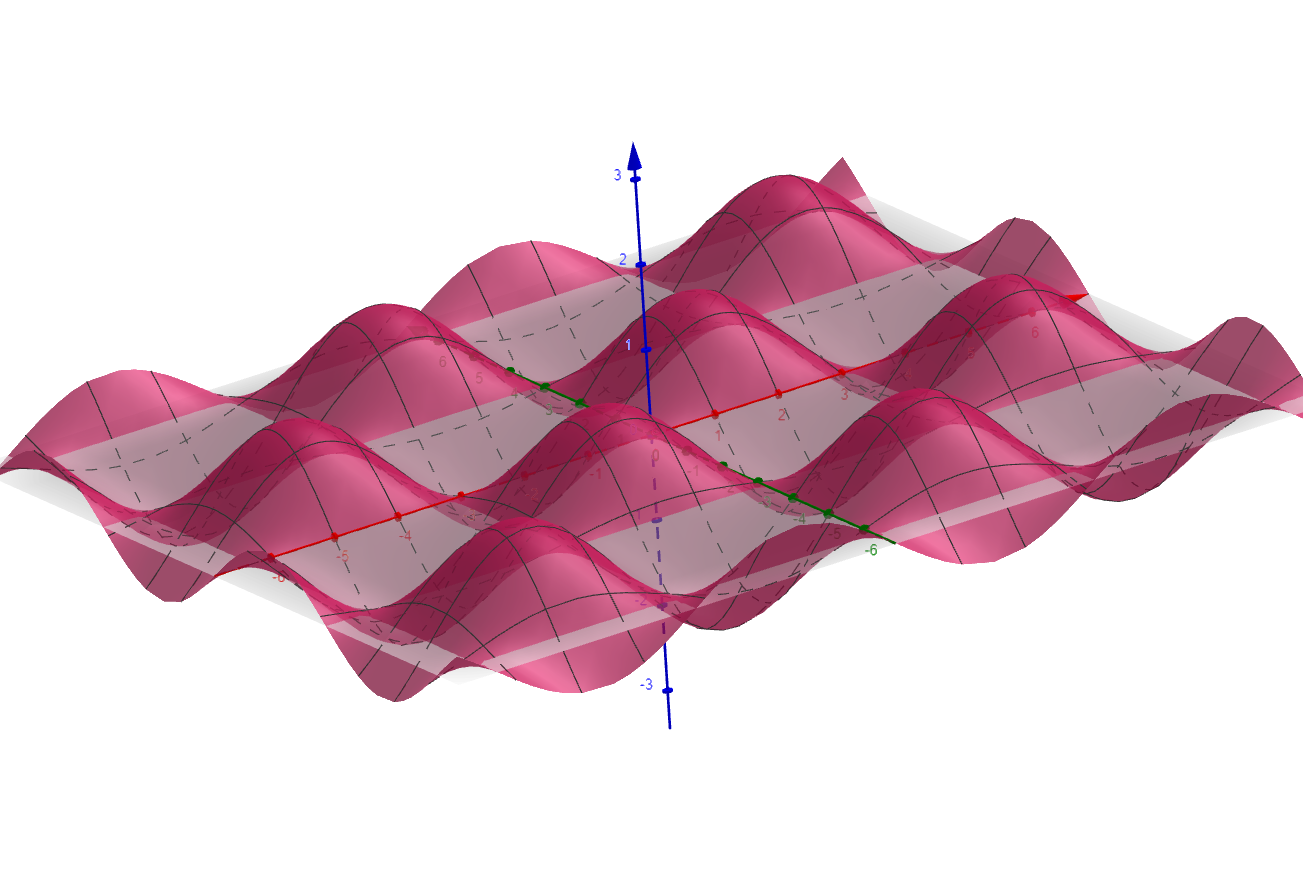
\includegraphics[scale=0.2]{Figuras/Semana11/seno}
    \caption{}
    \label{fig:enter-label}
\end{figure}
\end{example}

Por outro lado, como já dizemos, em muitos problemas, os domínios matemáticos das funções não coincidem com o conjunto no qual nos interessa estudar uma determinada função. Pode ocorrer que um máximo global de uma função esteja localizado fora do nosso domínio de interesse, ou nem exista. No entanto, mesmo nessas situações, é possível identificar pontos em que, dentro de vizinhanças limitadas desses pontos, os valores da função se mantêm sempre acima ou abaixo do valor da função no próprio ponto. Vejamos um exemplo.
\begin{example}{}{}
Seja $f(x,y)=(x^2+y^2)\ln(9-x^2-y^2)$. Pelas propriedades do logaritmo sabemos que $f$ é não negativa sobre o círculo de raio 3. Além disso, dentro desse círculo a função atinge o valor $0$ apenas em $(0,0)$, sendo um mínimo global se restringimos a análise da função apenas a esse círculo. Por outro lado, a função vai para menos infinito quando $(x,y)\rightarrow (\pm \infty,\pm \infty)$ e, portanto, a origem não é um mínimo global da função. 
\begin{figure}[H]
    \centering
    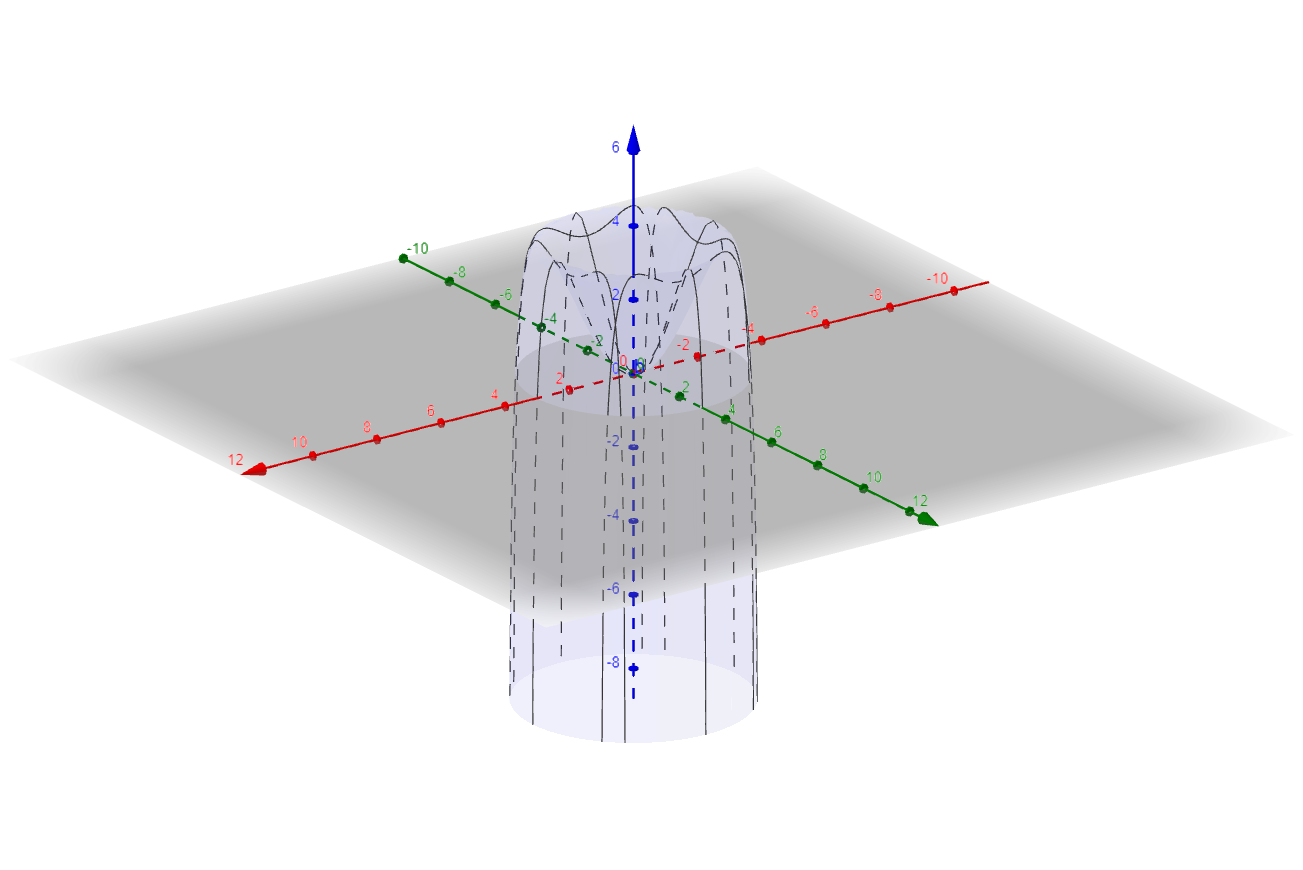
\includegraphics[width=\linewidth]{Figuras/Semana11/log_.png}
    \caption{}
    \label{fig:log}
\end{figure}
\end{example}

\pagebreak 
Esse tipo de pontos são de grande importância, pois,  embora não sejam extremos globais, podem ser suficientes para resolver determinado problema que esteja sendo  investigando. Se faz necessária, portanto, as seguintes definições. 
\begin{definition}{Mínimo local}{}
Um ponto \((x_1^0, x_2^0, \ldots, x_n^0)\) é considerado um \textit{mínimo local}\index{minimo@mínimo!local} de uma função \(f:D\subset\R^n\to\R\) se existe uma vizinhança em torno de \((x_1^0, x_2^0, \ldots, x_n^0)\) na qual \(f(x_1, x_2, \ldots, x_n)\leq f(x_1, x_2, \ldots, x_n)\) para todo $(x_1, x_2, \ldots, x_n)$ dentro dessa vizinhança, exceto possivelmente em \((x_1, x_2, \ldots, x_n)\) próprio.     
\end{definition}


Analogamente, temos o conceito de máximo local. 
\begin{definition}{Máximo local}{}
Um ponto \((x_1^0, x_2^0, \ldots, x_n^0)\) é considerado um \textit{máximo local}\index{maximo@máximo!local} de uma função \(f:D\subset\R^n\to\R\) se existe uma vizinhança em torno de \((x_1^0, x_2^0, \ldots, x_n^0)\) na qual \(f(x_1, x_2, \ldots, x_n)\geq f(x_1, x_2, \ldots, x_n)\) para todo $(x_1, x_2, \ldots, x_n)$ dentro dessa vizinhança, exceto possivelmente em \((x_1, x_2, \ldots, x_n)\) próprio.     
\end{definition}

Observe que os extremos globais em particular são extremos locais. 

\section{}
Até agora estudamos funções cujos valores extremos são facilmente determinados a partir da própria expressão da função. Em problemas da vida real, onde as funções modelam fenômenos complexos, é muito mais difícil determinar esses valores. Então precisamos buscar alternativas para determinar os pontos onde a função atinge seus extremos. O seguinte resultado é uma condição necessária satisfeita por extremos locais, que nos dá um primero passo na búsqueda por esses pontos. 
\begin{theorem}{}{}
    Se \((x_1^0, x_2^0, \ldots, x_n^0)\) é um {mínimo ou um máximo  local}\index{minimo@mínimo!local} de uma função diferenciável \(f:D\subset\R^n\to\R\), então $\nabla f(x_1^0, x_2^0, \ldots, x_n^0)=0$. 
\end{theorem}
\begin{proof}
Suponhamos que $\Point{x}_0=(x_1^0, x_2^0, \ldots, x_n^0)$ seja um mínimo local de $f$. Para cada $i=1,...,n$, consideremos a função de uma variável $$f_i(t)=f(x_1^0,\dots,x_{i-1}^0,x_i^0+t,x_{i+1}^0,\dots,x_n^0),$$ onde $t$ é suficientemente pequeno para que $(x_1^0,\dots,x_{i-1}^0,x_i^0+t,x_{i+1}^0,\dots,x_n^0)$ esteja contido em $D$. Obviamente $t=0$ é um mínimo dessa função, e de Cálculo I sabemos que $f_i'(0)=0$. Usando a regra da cadeia temos que 
$$f_i'(0) = \sum_{j=1}^n\dfrac{\partial f}{\partial x_j}(\Point{x}_0) \cdot x_j'(t) = \dfrac{\partial f}{\partial x_i}(\Point{x}_0). $$
Logo, todas as derivadas parciais são nula como desejado. 
\end{proof}



\todo[inline]{Observar aquí que o teorema implica que o plano tangente ao gráfico de uma função diferenciável nos seus máximos e mínimos locais é um plano horizontal porque o vetor normal é $N=(0,0,\dots,1)$.}

Observe que existem funções que podem não ser diferenciáveis nos seus pontos de máximo ou mínimo locais (ou globais). Por exemplo, a função de Cobb-Douglass, $u(x,y)=x^{\frac{1}{2}}y^{\frac{1}{2}}$, tem um mínimo global na origem e não é diferenciável na origem. A função $f(x,y)=\sqrt{x^2+y^2}$ também não é diferenciável na origem, que é seu mínimo global. Ou seja, o teorema pode ser aplicado às funções que sejam diferenciáveis, como indica a hipótese. Em outros casos são necessárias outras análises. 

\begin{example}{}{}
No caso da função definida em \eqref{eq:minimo_global}  temos que $\nabla f (x,y)=(2x,2y)$ que se anula na origem. No caso da função definida em \eqref{eq:maximo_global} temos $\nabla f(x,y)=\left(-2xe^{-x^2-y^2},-2ye^{-x^2-y^2}\right)$, que também se anula na origem. 
\end{example}

\begin{definition}{Ponto crítico}{}
    Um ponto $\Point{x}_0$ do domínio de uma função $f:D\subset \R^n\to\R$ de classe $C^2$ que satisfaz $\nabla f (\Point{x}_0)=0 $ é chamado de \textit{ponto crítico}\index{ponto!crítico} de $f$. 
\end{definition}

Observe agora que o Teorema 1.5 não diz que todo ponto crítico seja um máximo e um mínimo local. Vejamos um contraexemplo. 
\begin{example}{Sela de cavalo}{}
Considere a função    
\begin{equation}\label{eq:sela}
f(x,y)=x^2-y^2.
\end{equation}
Temos que $\nabla f(x,y)=(2x,-2y)$ que se anula na origem, porém, a origem não é nem um máximo nem um mínimo dessa função como vamos mostrar a continuação. 

Analizemos a curva plana que é interseção do gráfico de $f$ com o plano $y=0$, em vermelho na Figura \ref{fig:sela1}. 
\begin{figure}[H]
    \centering
    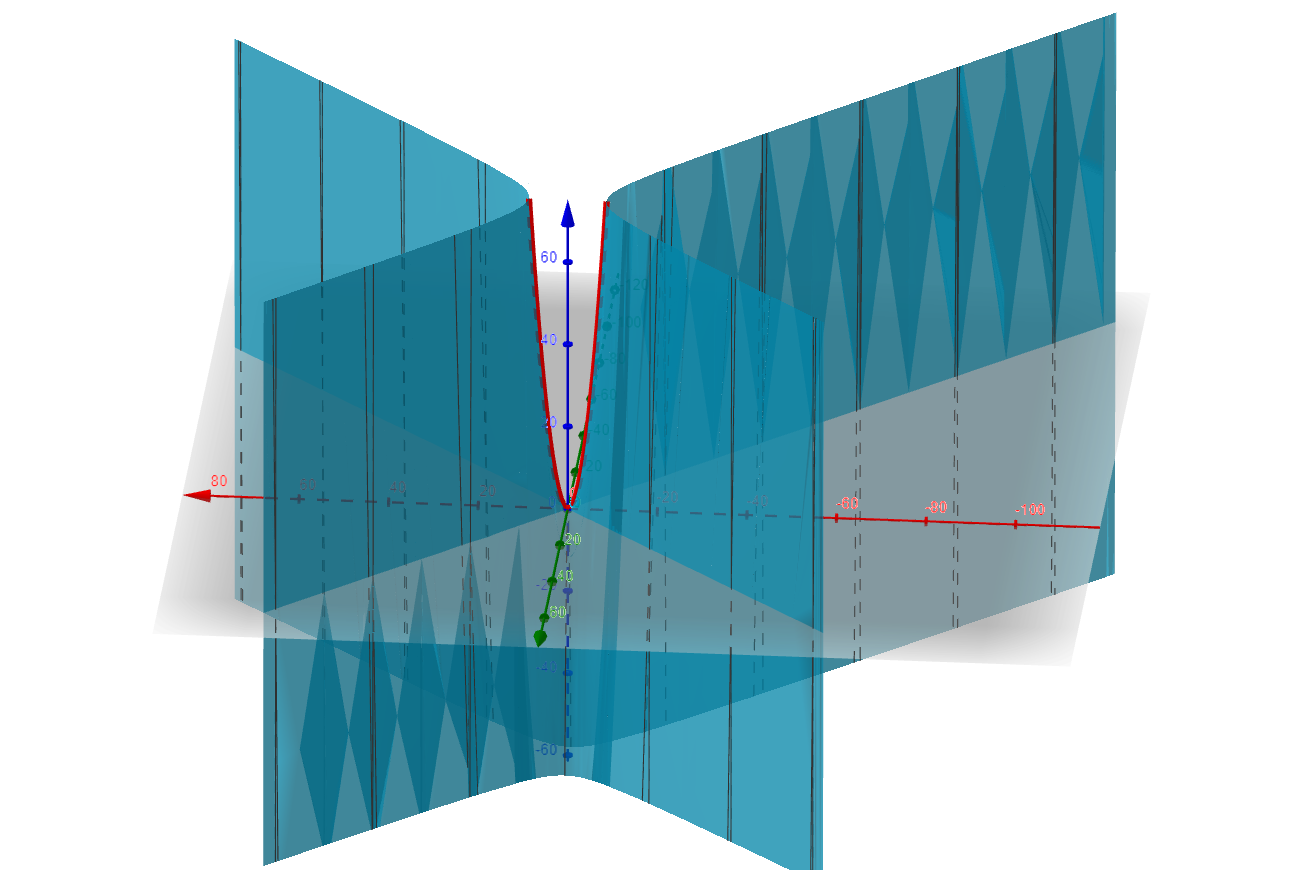
\includegraphics[scale=0.25]{Figuras/Semana11/sela1}
    \caption{}
    \label{fig:sela1}
\end{figure}
Visualmente observamos que essa curva tem uma altura mínima igual a zero, e de fato, no plano de equação $y=0$, tal curva é o gráfico da função de uma variável $h(x)=f(x,0)=x^2$, que obviamente tem um mínimo em $x=0$. Daí, sobre os pontos dessa curva temos
\begin{equation}
    f(x,0)=h(x)\geq h(0)=f(0,0).
    \label{eq:sela1}
\end{equation}
Por outro lado, na Figura \ref{fig:sela2} se mostra a curva que é o gráfico no plano de equação $x=0$ da função $\Tilde{h}(y)=f(0,y)=-y^2$, que tem um máximo em  $y=0$. 
\begin{figure}[H]
    \centering
    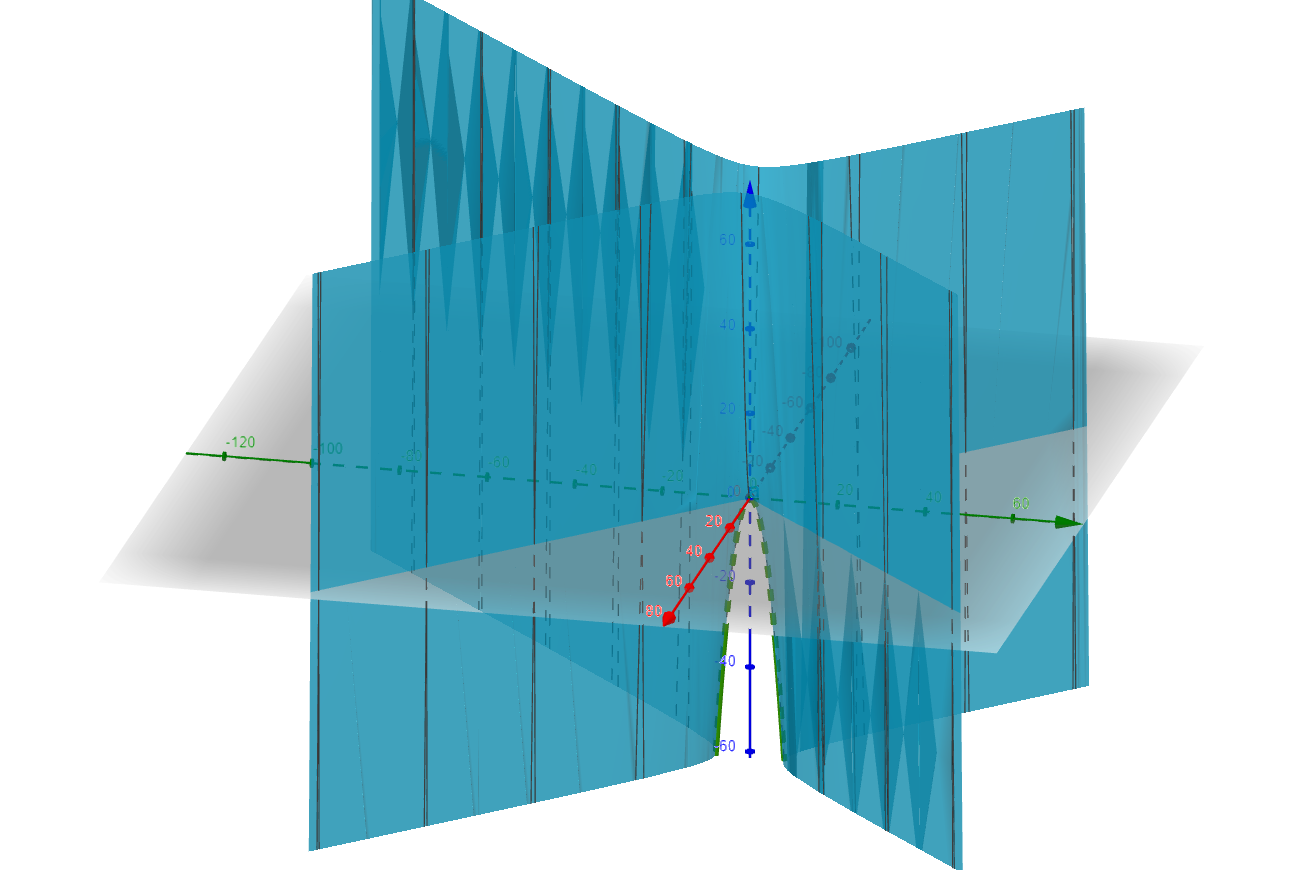
\includegraphics[scale=0.25]{Figuras/Semana11/sela2}
    \caption{}
    \label{fig:sela2}
\end{figure}
Desta forma, 
\begin{equation}
f(0,y)=\Tilde{h}(y)\leq \Tilde{h}(0)=f(0,0).
\label{eq:sela2}
\end{equation}

As equações \eqref{eq:sela1} e \eqref{eq:sela2} implicam que $(0,0)$ não é nem máximo nem mínimo dessa função, pois implicam que $f$ não satisfaz nem a definição de mínimo local nem a definição de máximo local. 
\end{example}

\begin{definition}{}{}
    Um ponto crítico de uma função que não é nem máximo e nem mínimo local é chamado de \textit{sela}\index{sela}.  
\end{definition}

\section{Classificação dos pontos críticos}
O Teorema 1.4 fornece o primeiro passo na busca por extremos locais de uma função diferenciável. No entanto, para determinar se um ponto crítico é um máximo ou mínimo, dependendo do contexto, precisamos de ferramentas adicionais.

Para isso, observemos que o Teorema de Taylor garante que se $\Point{x}_0=(x_1^0,x_2^0,\dots,x_n^0)$ é um ponto crítico de uma função duas vezes diferenciável $f:D\subset\R^n\to\R$, então para todo $\Point{x}=(x_1,x_2,\dots,x_n)$ suficientemente próximo de $\Point{x}_0$ temos que
\begin{align*}
\!\!f(\Point{x})-f(\Point{x}_0)&= \sum_{i=0}^n \underbrace{\dfrac{\partial f}{\partial x_i} (\Point{x}_0)}_{0} (x_i-x_i^0) + \frac{1}{2}\sum_{i,j=1}^n \dfrac{\partial ^2 f}{\partial x_i \partial x_j}(\Point{x}_0)(x_i-x_i^0)(x_j-x_j^0) + R(\Point{x})\\
&= \frac{1}{2} \sum_{i,j=1}^n \dfrac{\partial ^2 f}{\partial x_i \partial x_j}(\Point{x}_0)(x_i-x_i^0)(x_j-x_j^0) + R(\Point{x})
\end{align*}
sendo que
\begin{equation}\label{eq:resto}
    \lim_{\Point x \rightarrow \Point{x}_0} \dfrac{R(\Point{x})}{\|\Point{x}-\Point{x}_0\|^2}=0. 
\end{equation}

Se a forma quadrática 
$$Q(\Point{x})=\sum_{i,j=1}^n \dfrac{\partial ^2 f}{\partial x_i \partial x_j}(\Point{x}_0)x_i x_j=\Point{x}^T \Hess f(\Point{x}_0)\Point{x}$$
for estritamente definida positiva, isto é, se $Q(\Point{x})>0$ para todo $\Point{x}\neq 0$, então $\Point{x}_0$ é um mínimo local. De fato, como
$$\lim_{\Point x \rightarrow \Point{x}_0} \dfrac{Q(\Point x -  \Point{x}_0)}{\norm{\Point x -  \Point{x}_0}^2} > 0$$
e vale \eqref{eq:resto}, então podemos ``encolher'' a vizinhança em torno de $\Point{x}_0$ de forma tal que  
$$f(\Point{x})-f(\Point{x}_0)=Q(\Point{x}-\Point{x}_0)-R(\Point{x})>0.$$ 

Analogamente, se $Q$ for estritamente definida negativa temos que $\Point{x}_0$ é um máximo local. 

\begin{example}{}{}
Observe como no caso da função definida em \eqref{eq:minimo_global} temos que 
$$\Hess f(0,0)= \begin{pmatrix}
    2&0\\
    0&2
\end{pmatrix},$$
logo,
$$Q(x,y)=2x^2+2y^2,$$
que é estritamente positiva para todo $(x,y)\neq (0,0)$. De qualquer forma, já sabíamos que a origem é um mínimo global. 

Analogamente, para a função definida em \eqref{eq:maximo_global} temos que 
$$\dfrac{\partial^2 f}{\partial x^2}(x,y)=-2(1-2x^2)e^{-x^2-y^2},$$
$$\dfrac{\partial^2 f}{\partial x \partial y}(x,y)=\dfrac{\partial^2 f}{\partial y \partial x}(x,y)=4xye^{-x^2-y^2}$$
e
$$\dfrac{\partial^2 f}{\partial x^2}(x,y)=-2(1-2y^2)e^{-x^2-y^2}.$$
Assim, 
$$\Hess f(0,0)= 
\begin{pmatrix}
    -2&0\\
    0&-2
\end{pmatrix}$$
e, portanto, 
$$Q(x,y) = -2x^2-2 y^2$$
que é estritamente negativa fora da origem. 
\end{example}
Para aqueles que já possuem conhecimento sobre autovalores de matrizes, observem que em ambos os casos do exemplo anterior a matriz Hessiana é a matriz diagonal contendo um único autovalor de multiplicidade 2. Lembrem que para determinar se uma forma quadrática é estritamente definida positiva ou negativa é suficiente analisar o sinal dos autovalores da matriz que a representa. 

\pagebreak
Vejamos outro exemplo
\begin{example}{}{}
Consideremos a função
\begin{equation}\label{ilust_locais}
    f(x,y)=x^4+y^4 -4xy + 1
\end{equation} 

Temos
$$\nabla f (x,y) = (4x^3-4y,4y^3-4x).$$
Para determinar os pontos críticos devemos resolver os sistema de equações
$$\begin{cases}
    4x^3-4y=0,\\
    4y^3-4x=0,
\end{cases}$$
cujas soluções são $p_1=(1,1)$, $p_2=(-1,-1)$ e $p_3=(0,0)$. Para identificar quem é máximo e mínimo, devemos determinar a forma quadrática $Q$.
Temos 
$$\dfrac{\partial^2 f }{\partial x^2}(x,y)=12x^2,\quad 
\dfrac{\partial^2 f }{\partial x\partial y}(x,y)=\dfrac{\partial^2 f }{\partial y\partial x}(x,y)=-4 
\quad \mbox{e} \quad \dfrac{\partial^2 f }{\partial y^2}(x,y)=12 y^2.$$
Logo,
$$\Hess f(1,1)= \Hess f(-1,-1)=
\begin{pmatrix}
    12&-4\\
    -4&12
\end{pmatrix},$$
assim, em ambos casos temos que 
$$Q(x,y)=12x^2-8xy+12y^2.$$
Nesse caso não podemos determinar a simples vista se $Q$ tem um sinal bem definido. Façamos uma pequena análise:
Se $x=0$ temos que $Q>0$. Supondo agora que $x\neq 0 $ 
podemos considerar que $p(y)=3x^2-2xy+3y^2$ é um  polinômio em $y$ para cada $x$ fixado. Assim, o discriminante é 
$D= 4x^2 -4 \cdot 3 \cdot 3x^2 =-32 x^2<0,$ o que implica que tal polinômio não tem raízes reais. Isso significa que ele não muda de sinal e, portanto, $p(y)$ terá o mesmo sinal do caso em que $y=x$, ou seja, $p(x)=3x^2-2x\cdot x+3x^2=4x^2>0$. Como para cada $x$ fixado $Q(x,y)>0$ para todo $y\in\R$, concluímos que $Q(x,y)>0$ para todo $(x,y)\in\R^2$. Portanto $(1,1)$ e $(-1,-1)$ são mínimos locais. 

\medskip 

Por outro lado, 
$$\Hess f(0,0)= 
\begin{pmatrix}
    0&-4\\
    -4&0
\end{pmatrix}$$
Daí, 
$Q(x,y)=-8xy$ cujo sinal não é constante, depende do sinal de $x$ e de $y$. Observe na figura a seguir que a origem é uma sela. 


\begin{figure}[H]
    \centering
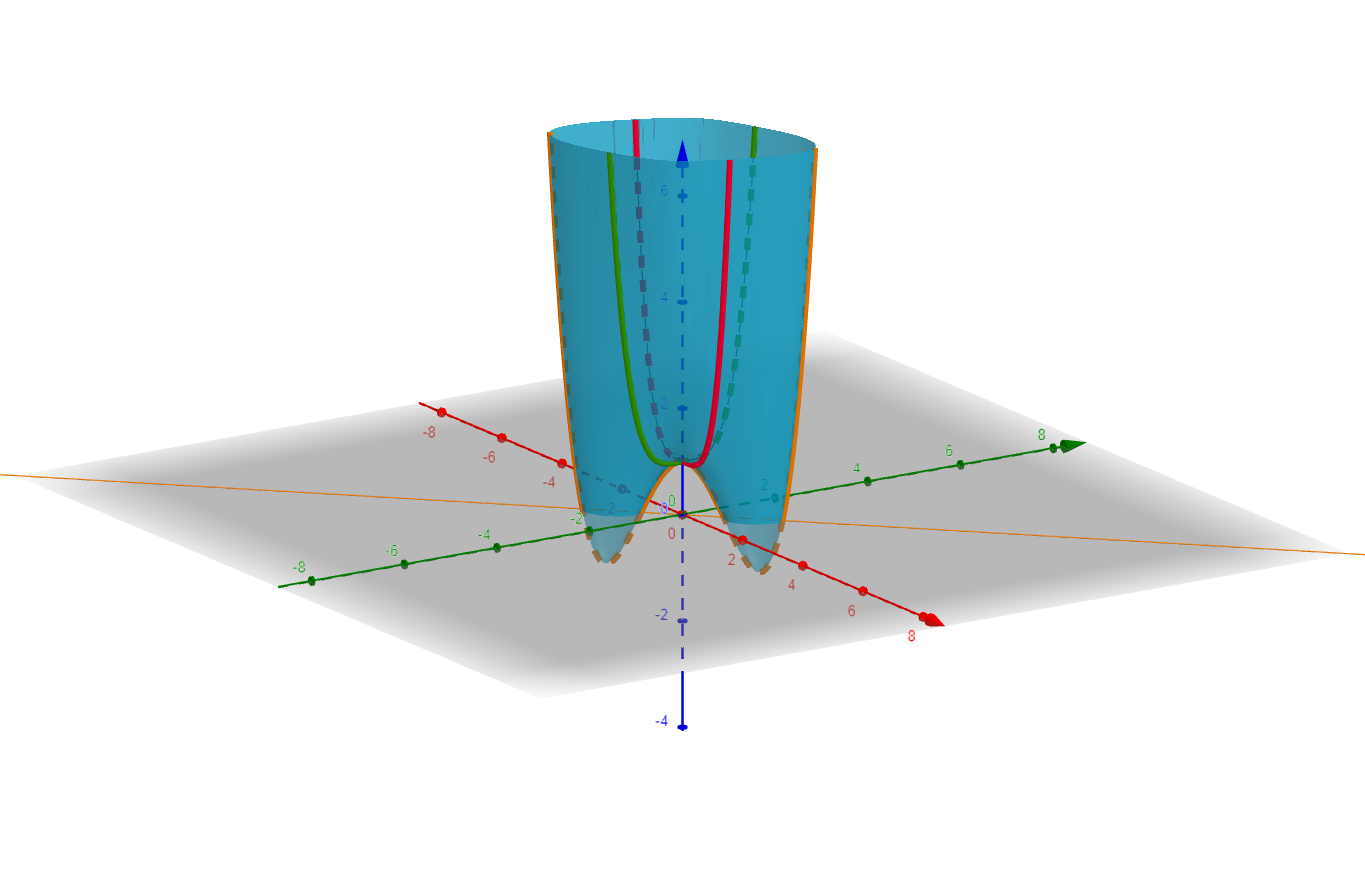
\includegraphics[scale=0.2]{Figuras/Semana11/fig1}
\end{figure}
\end{example}

No exemplo anterior, observamos que a determinação do sinal da forma quadrática $Q$ foi mais desafiadora em comparação ao Exemplo 1.5. Em situações gerais, a análise direta do sinal pode ser bastante complicada, senão impossível, dependendo da expressão da função em análise. Portanto, é de grande importância possuir métodos que permitam determinar se uma forma quadrática é positiva ou negativa sem depender de análises detalhadas.

Para chegar no caso geral, comecemos pelo caso em que $f$ é uma função de duas variáveis ($n=2$) e de classe $C^2$. Seja $(x_0,y_0)$ um ponto crítico, então
\begin{equation}\label{eq:q}
Q(x,y) =\frac{\partial^2f}{\partial x^2}(x_0,y_0)x^2 + 2 \frac{\partial^2f}{\partial x\partial y}(x_0,y_0)xy + \frac{\partial^2f}{\partial y^2}(x_0,y_0)y^2. 
\end{equation}
Façamos uma análise parecida com a que fizemos no Exemplo 1.6. Fixemos $x\neq 0$  e consideremos o seguinte polinômio em $y$:
$$p(y)=\frac{\partial^2f}{\partial x^2}(x_0,y_0)x^2 + 2 \frac{\partial^2f}{\partial x\partial y}(x_0,y_0)xy + \frac{\partial^2f}{\partial y^2}(x_0,y_0)y^2.$$
Temos
\begin{align*}
D & = \underbrace{4\left(\frac{\partial^2f}{\partial x\partial y}(x_0,y_0)\right)^2x^2}_{b^2}-4\cdot \underbrace{\frac{\partial^2f}{\partial y^2}(x_0,y_0)}_{a}\cdot \underbrace{\frac{\partial^2f}{\partial x^2}(x_0,y_0)x^2}_c.\\
&= -4x^2\left( \underbrace{\frac{\partial^2f}{\partial x^2}(x_0,y_0) \frac{\partial^2f}{\partial y^2}(x_0,y_0)-\left(\frac{\partial^2f}{\partial x\partial y}(x_0,y_0)\right)^2}_{\det \left(\Hess f(x_0,y_0)\right)}\right). 
\end{align*}
%Se $(x_0,y_0)$ for um máximo ou um mínimo, então $D$ tem que ser estritamente negativo, pois 
Observe que a condição ``$Q>0$ ou $Q<0$'' implica que $p(y)$ não tem raízes reais. Portanto, $\det \left(\Hess f(x_0,y_0)\right)$ tem que ser estritamente positivo. 

%Se $\det \left(\Hess f(x_0,y_0)\right)$ for não negativo, então $Q$ muda de sinal

Além disso, observe que se $\det \left(\Hess f(x_0,y_0)\right)>0$, então necessariamente $ \frac{\partial^2f}{\partial x^2}(x_0,y_0)$ e $ \frac{\partial^2f}{\partial x^2}(x_0,y_0)$ não se anulam e tem o mesmo sinal! Assim, $Q(x,y)$ tem o mesmo sinal que $Q(1,0)=\frac{\partial^2f}{\partial x^2}(x_0,y_0)$ (que é o mesmo sinal de $Q(0,1)=\frac{\partial^2f}{\partial y^2}(x_0,y_0)$). 

Chegamos, portanto, ao seguinte critério de classificação:
\begin{theorem}{Critério de classificação de pontos críticos para funções de duas variáveis}{}
Sejam $f:D\subset \R^2\to\R$ uma função de classe $C^2$ e $(x_0,y_0)\in D$ um ponto crítico de $f$. Então
\begin{itemize}
\item Se $\det (\Hess f(x_0,y_0))>0$ e $\frac{\partial^2f}{\partial x^2}(x_0,y_0)>0$, então $(x_0,y_0)$ é um mínimo local (pois $Q$ é estritamente definida positiva).
\item Se $\det (\Hess f(x_0,y_0))>0$ e $\frac{\partial^2f}{\partial x^2}(x_0,y_0)<0$, então $(x_0,y_0)$ é um máximo local (pois $Q$ é estritamente definida negativa).
\item Se $\det (\Hess f(x_0,y_0))<0$, então $(x_0,y_0)$ é uma sela. 
\end{itemize}
\end{theorem}

Observe que se $\det (\Hess f(x_0,y_0))=0$ não podemos dizer nada sobre a natureza do ponto crítico. %De fato, neste caso, $D=0$ e $p(y)$ teria uma única raiz para cada $x$ fixado, digamos $y_x$ (porque tal $y$ depende de $x$). Ou seja, para cada $x$ existe $y_x$ tal que  $Q(x,y_x)=0$. Mas isso não diz nada sobre o sinal de $Q$ poderia ser positivo sempre, neste caso necessariamente   



% 1.5 Convexity $=$ convexity along all lines

Theorem 1. A function $f: \mathbb{R}^n \rightarrow \mathbb{R}$ is convex if and only if the function $g: \mathbb{R} \rightarrow \mathbb{R}$ given by $g(t)=f(x+t y)$ is convex (as a univariate function) for all $x$ in domain of $f$ and all $y \in \mathbb{R}^n$. (The domain of $g$ here is all $t$ for which $x+$ ty is in the domain of $f$.)

Proof: This is straightforward from the definition.


\url{https://www.princeton.edu/~aaa/Public/Teaching/ORF523/S16/ORF523_S16_Lec7_gh.pdf}


%\printindex

\end{document}
